\documentclass[twoside]{book}

% Packages required by doxygen
\usepackage{fixltx2e}
\usepackage{calc}
\usepackage{doxygen}
\usepackage[export]{adjustbox} % also loads graphicx
\usepackage{graphicx}
\usepackage[utf8]{inputenc}
\usepackage{makeidx}
\usepackage{multicol}
\usepackage{multirow}
\PassOptionsToPackage{warn}{textcomp}
\usepackage{textcomp}
\usepackage[nointegrals]{wasysym}
\usepackage[table]{xcolor}

% Font selection
\usepackage[T1]{fontenc}
\usepackage[scaled=.90]{helvet}
\usepackage{courier}
\usepackage{amssymb}
\usepackage{sectsty}
\renewcommand{\familydefault}{\sfdefault}
\allsectionsfont{%
  \fontseries{bc}\selectfont%
  \color{darkgray}%
}
\renewcommand{\DoxyLabelFont}{%
  \fontseries{bc}\selectfont%
  \color{darkgray}%
}
\newcommand{\+}{\discretionary{\mbox{\scriptsize$\hookleftarrow$}}{}{}}

% Page & text layout
\usepackage{geometry}
\geometry{%
  a4paper,%
  top=2.5cm,%
  bottom=2.5cm,%
  left=2.5cm,%
  right=2.5cm%
}
\tolerance=750
\hfuzz=15pt
\hbadness=750
\setlength{\emergencystretch}{15pt}
\setlength{\parindent}{0cm}
\setlength{\parskip}{3ex plus 2ex minus 2ex}
\makeatletter
\renewcommand{\paragraph}{%
  \@startsection{paragraph}{4}{0ex}{-1.0ex}{1.0ex}{%
    \normalfont\normalsize\bfseries\SS@parafont%
  }%
}
\renewcommand{\subparagraph}{%
  \@startsection{subparagraph}{5}{0ex}{-1.0ex}{1.0ex}{%
    \normalfont\normalsize\bfseries\SS@subparafont%
  }%
}
\makeatother

% Headers & footers
\usepackage{fancyhdr}
\pagestyle{fancyplain}
\fancyhead[LE]{\fancyplain{}{\bfseries\thepage}}
\fancyhead[CE]{\fancyplain{}{}}
\fancyhead[RE]{\fancyplain{}{\bfseries\leftmark}}
\fancyhead[LO]{\fancyplain{}{\bfseries\rightmark}}
\fancyhead[CO]{\fancyplain{}{}}
\fancyhead[RO]{\fancyplain{}{\bfseries\thepage}}
\fancyfoot[LE]{\fancyplain{}{}}
\fancyfoot[CE]{\fancyplain{}{}}
\fancyfoot[RE]{\fancyplain{}{\bfseries\scriptsize Generated by Doxygen }}
\fancyfoot[LO]{\fancyplain{}{\bfseries\scriptsize Generated by Doxygen }}
\fancyfoot[CO]{\fancyplain{}{}}
\fancyfoot[RO]{\fancyplain{}{}}
\renewcommand{\footrulewidth}{0.4pt}
\renewcommand{\chaptermark}[1]{%
  \markboth{#1}{}%
}
\renewcommand{\sectionmark}[1]{%
  \markright{\thesection\ #1}%
}

% Indices & bibliography
\usepackage{natbib}
\usepackage[titles]{tocloft}
\setcounter{tocdepth}{3}
\setcounter{secnumdepth}{5}
\makeindex

% Hyperlinks (required, but should be loaded last)
\usepackage{ifpdf}
\ifpdf
  \usepackage[pdftex,pagebackref=true]{hyperref}
\else
  \usepackage[ps2pdf,pagebackref=true]{hyperref}
\fi
\hypersetup{%
  colorlinks=true,%
  linkcolor=blue,%
  citecolor=blue,%
  unicode%
}

% Custom commands
\newcommand{\clearemptydoublepage}{%
  \newpage{\pagestyle{empty}\cleardoublepage}%
}

\usepackage{caption}
\captionsetup{labelsep=space,justification=centering,font={bf},singlelinecheck=off,skip=4pt,position=top}

%===== C O N T E N T S =====

\begin{document}

% Titlepage & ToC
\hypersetup{pageanchor=false,
             bookmarksnumbered=true,
             pdfencoding=unicode
            }
\pagenumbering{alph}
\begin{titlepage}
\vspace*{7cm}
\begin{center}%
{\Large P\+O\+P\+BL 5 }\\
\vspace*{1cm}
{\large Generated by Doxygen 1.8.14}\\
\end{center}
\end{titlepage}
\clearemptydoublepage
\pagenumbering{roman}
\tableofcontents
\clearemptydoublepage
\pagenumbering{arabic}
\hypersetup{pageanchor=true}

%--- Begin generated contents ---
\chapter{Namespace Index}
\section{Packages}
Here are the packages with brief descriptions (if available)\+:\begin{DoxyCompactList}
\item\contentsline{section}{\mbox{\hyperlink{namespacesimulator}{simulator}} }{\pageref{namespacesimulator}}{}
\item\contentsline{section}{\mbox{\hyperlink{namespacetest}{test}} }{\pageref{namespacetest}}{}
\end{DoxyCompactList}

\chapter{Hierarchical Index}
\section{Class Hierarchy}
This inheritance list is sorted roughly, but not completely, alphabetically\+:\begin{DoxyCompactList}
\item \contentsline{section}{simulator.\+Lista\+Segmento}{\pageref{classsimulator_1_1_lista_segmento}}{}
\item \contentsline{section}{test.\+Manager\+Test}{\pageref{classtest_1_1_manager_test}}{}
\item \contentsline{section}{simulator.\+Pedido}{\pageref{classsimulator_1_1_pedido}}{}
\item \contentsline{section}{test.\+Pedido\+Test}{\pageref{classtest_1_1_pedido_test}}{}
\item \contentsline{section}{simulator.\+Principal}{\pageref{classsimulator_1_1_principal}}{}
\item \contentsline{section}{simulator.\+Producto}{\pageref{classsimulator_1_1_producto}}{}
\item \contentsline{section}{test.\+Producto\+Test}{\pageref{classtest_1_1_producto_test}}{}
\item \contentsline{section}{simulator.\+Segmento}{\pageref{classsimulator_1_1_segmento}}{}
\item Thread\begin{DoxyCompactList}
\item \contentsline{section}{simulator.\+Manager}{\pageref{classsimulator_1_1_manager}}{}
\item \contentsline{section}{simulator.\+Vehiculo}{\pageref{classsimulator_1_1_vehiculo}}{}
\end{DoxyCompactList}
\item \contentsline{section}{simulator.\+Workstation}{\pageref{classsimulator_1_1_workstation}}{}
\item Easy\+Mock\+Support\begin{DoxyCompactList}
\item \contentsline{section}{test.\+Vehicles\+Test}{\pageref{classtest_1_1_vehicles_test}}{}
\end{DoxyCompactList}
\end{DoxyCompactList}

\chapter{Class Index}
\section{Class List}
Here are the classes, structs, unions and interfaces with brief descriptions\+:\begin{DoxyCompactList}
\item\contentsline{section}{\mbox{\hyperlink{classsimulator_1_1_lista_segmento}{simulator.\+Lista\+Segmento}} }{\pageref{classsimulator_1_1_lista_segmento}}{}
\item\contentsline{section}{\mbox{\hyperlink{classsimulator_1_1_manager}{simulator.\+Manager}} }{\pageref{classsimulator_1_1_manager}}{}
\item\contentsline{section}{\mbox{\hyperlink{classtest_1_1_manager_test}{test.\+Manager\+Test}} }{\pageref{classtest_1_1_manager_test}}{}
\item\contentsline{section}{\mbox{\hyperlink{classsimulator_1_1_pedido}{simulator.\+Pedido}} }{\pageref{classsimulator_1_1_pedido}}{}
\item\contentsline{section}{\mbox{\hyperlink{classtest_1_1_pedido_test}{test.\+Pedido\+Test}} }{\pageref{classtest_1_1_pedido_test}}{}
\item\contentsline{section}{\mbox{\hyperlink{classsimulator_1_1_principal}{simulator.\+Principal}} }{\pageref{classsimulator_1_1_principal}}{}
\item\contentsline{section}{\mbox{\hyperlink{classsimulator_1_1_producto}{simulator.\+Producto}} }{\pageref{classsimulator_1_1_producto}}{}
\item\contentsline{section}{\mbox{\hyperlink{classtest_1_1_producto_test}{test.\+Producto\+Test}} }{\pageref{classtest_1_1_producto_test}}{}
\item\contentsline{section}{\mbox{\hyperlink{classsimulator_1_1_segmento}{simulator.\+Segmento}} }{\pageref{classsimulator_1_1_segmento}}{}
\item\contentsline{section}{\mbox{\hyperlink{classtest_1_1_vehicles_test}{test.\+Vehicles\+Test}} }{\pageref{classtest_1_1_vehicles_test}}{}
\item\contentsline{section}{\mbox{\hyperlink{classsimulator_1_1_vehiculo}{simulator.\+Vehiculo}} }{\pageref{classsimulator_1_1_vehiculo}}{}
\item\contentsline{section}{\mbox{\hyperlink{classsimulator_1_1_workstation}{simulator.\+Workstation}} }{\pageref{classsimulator_1_1_workstation}}{}
\end{DoxyCompactList}

\chapter{File Index}
\section{File List}
Here is a list of all files with brief descriptions\+:\begin{DoxyCompactList}
\item\contentsline{section}{java/main/java/simulator/\mbox{\hyperlink{_lista_segmento_8java}{Lista\+Segmento.\+java}} }{\pageref{_lista_segmento_8java}}{}
\item\contentsline{section}{java/main/java/simulator/\mbox{\hyperlink{_manager_8java}{Manager.\+java}} }{\pageref{_manager_8java}}{}
\item\contentsline{section}{java/main/java/simulator/\mbox{\hyperlink{_pedido_8java}{Pedido.\+java}} }{\pageref{_pedido_8java}}{}
\item\contentsline{section}{java/main/java/simulator/\mbox{\hyperlink{_principal_8java}{Principal.\+java}} }{\pageref{_principal_8java}}{}
\item\contentsline{section}{java/main/java/simulator/\mbox{\hyperlink{_producto_8java}{Producto.\+java}} }{\pageref{_producto_8java}}{}
\item\contentsline{section}{java/main/java/simulator/\mbox{\hyperlink{_segmento_8java}{Segmento.\+java}} }{\pageref{_segmento_8java}}{}
\item\contentsline{section}{java/main/java/simulator/\mbox{\hyperlink{_vehiculo_8java}{Vehiculo.\+java}} }{\pageref{_vehiculo_8java}}{}
\item\contentsline{section}{java/main/java/simulator/\mbox{\hyperlink{_workstation_8java}{Workstation.\+java}} }{\pageref{_workstation_8java}}{}
\item\contentsline{section}{java/test/java/test/\mbox{\hyperlink{_manager_test_8java}{Manager\+Test.\+java}} }{\pageref{_manager_test_8java}}{}
\item\contentsline{section}{java/test/java/test/\mbox{\hyperlink{_pedido_test_8java}{Pedido\+Test.\+java}} }{\pageref{_pedido_test_8java}}{}
\item\contentsline{section}{java/test/java/test/\mbox{\hyperlink{_producto_test_8java}{Producto\+Test.\+java}} }{\pageref{_producto_test_8java}}{}
\item\contentsline{section}{java/test/java/test/\mbox{\hyperlink{_vehicles_test_8java}{Vehicles\+Test.\+java}} }{\pageref{_vehicles_test_8java}}{}
\end{DoxyCompactList}

\chapter{Namespace Documentation}
\hypertarget{namespacesimulator}{}\section{Package simulator}
\label{namespacesimulator}\index{simulator@{simulator}}
\subsection*{Classes}
\begin{DoxyCompactItemize}
\item 
class \mbox{\hyperlink{classsimulator_1_1_lista_segmento}{Lista\+Segmento}}
\item 
class \mbox{\hyperlink{classsimulator_1_1_manager}{Manager}}
\item 
class \mbox{\hyperlink{classsimulator_1_1_pedido}{Pedido}}
\item 
class \mbox{\hyperlink{classsimulator_1_1_principal}{Principal}}
\item 
class \mbox{\hyperlink{classsimulator_1_1_producto}{Producto}}
\item 
class \mbox{\hyperlink{classsimulator_1_1_segmento}{Segmento}}
\item 
class \mbox{\hyperlink{classsimulator_1_1_vehiculo}{Vehiculo}}
\item 
class \mbox{\hyperlink{classsimulator_1_1_workstation}{Workstation}}
\end{DoxyCompactItemize}

\hypertarget{namespacetest}{}\section{Package test}
\label{namespacetest}\index{test@{test}}
\subsection*{Classes}
\begin{DoxyCompactItemize}
\item 
class \mbox{\hyperlink{classtest_1_1_manager_test}{Manager\+Test}}
\item 
class \mbox{\hyperlink{classtest_1_1_pedido_test}{Pedido\+Test}}
\item 
class \mbox{\hyperlink{classtest_1_1_producto_test}{Producto\+Test}}
\item 
class \mbox{\hyperlink{classtest_1_1_vehicles_test}{Vehicles\+Test}}
\end{DoxyCompactItemize}

\chapter{Class Documentation}
\hypertarget{classsimulator_1_1_lista_segmento}{}\section{simulator.\+Lista\+Segmento Class Reference}
\label{classsimulator_1_1_lista_segmento}\index{simulator.\+Lista\+Segmento@{simulator.\+Lista\+Segmento}}


Collaboration diagram for simulator.\+Lista\+Segmento\+:\nopagebreak
\begin{figure}[H]
\begin{center}
\leavevmode
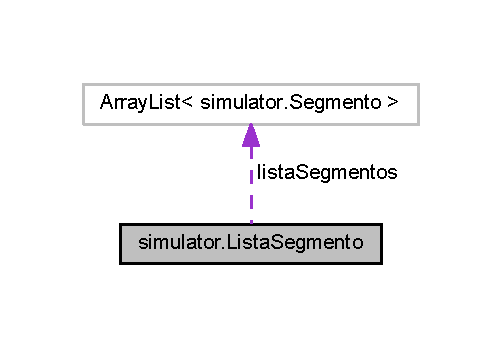
\includegraphics[width=241pt]{classsimulator_1_1_lista_segmento__coll__graph}
\end{center}
\end{figure}
\subsection*{Public Member Functions}
\begin{DoxyCompactItemize}
\item 
\mbox{\hyperlink{classsimulator_1_1_lista_segmento_af57e1ba52661c323d60e8a9f41f1042c}{Lista\+Segmento}} ()
\item 
void \mbox{\hyperlink{classsimulator_1_1_lista_segmento_a92b11e2e8cfcf09d45146e9771f87dea}{init}} ()
\item 
Array\+List$<$ \mbox{\hyperlink{classsimulator_1_1_segmento}{Segmento}} $>$ \mbox{\hyperlink{classsimulator_1_1_lista_segmento_ab699a3169c41d7baac0f86e47c0df66e}{get\+Lista\+Segmentos}} ()
\item 
void \mbox{\hyperlink{classsimulator_1_1_lista_segmento_a029655e5d0c31702beeba7834d024c43}{set\+Lista\+Segmentos}} (Array\+List$<$ \mbox{\hyperlink{classsimulator_1_1_segmento}{Segmento}} $>$ lista\+Segmentos)
\end{DoxyCompactItemize}


\subsection{Detailed Description}
This is the \mbox{\hyperlink{classsimulator_1_1_lista_segmento}{Lista\+Segmento}} class which has an array\+List of segments The list initialized all the parkings and workstations

\begin{DoxyAuthor}{Author}
Joseba Carnicero, Aitor Eizmendi, Jon Mugica and Marcos Azkarate 
\end{DoxyAuthor}


Definition at line 13 of file Lista\+Segmento.\+java.



\subsection{Constructor \& Destructor Documentation}
\mbox{\Hypertarget{classsimulator_1_1_lista_segmento_af57e1ba52661c323d60e8a9f41f1042c}\label{classsimulator_1_1_lista_segmento_af57e1ba52661c323d60e8a9f41f1042c}} 
\index{simulator\+::\+Lista\+Segmento@{simulator\+::\+Lista\+Segmento}!Lista\+Segmento@{Lista\+Segmento}}
\index{Lista\+Segmento@{Lista\+Segmento}!simulator\+::\+Lista\+Segmento@{simulator\+::\+Lista\+Segmento}}
\subsubsection{\texorpdfstring{Lista\+Segmento()}{ListaSegmento()}}
{\footnotesize\ttfamily simulator.\+Lista\+Segmento.\+Lista\+Segmento (\begin{DoxyParamCaption}{ }\end{DoxyParamCaption})}



Definition at line 17 of file Lista\+Segmento.\+java.

Here is the call graph for this function\+:\nopagebreak
\begin{figure}[H]
\begin{center}
\leavevmode
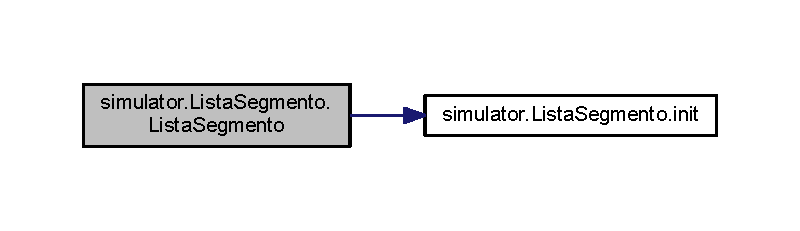
\includegraphics[width=350pt]{classsimulator_1_1_lista_segmento_af57e1ba52661c323d60e8a9f41f1042c_cgraph}
\end{center}
\end{figure}


\subsection{Member Function Documentation}
\mbox{\Hypertarget{classsimulator_1_1_lista_segmento_ab699a3169c41d7baac0f86e47c0df66e}\label{classsimulator_1_1_lista_segmento_ab699a3169c41d7baac0f86e47c0df66e}} 
\index{simulator\+::\+Lista\+Segmento@{simulator\+::\+Lista\+Segmento}!get\+Lista\+Segmentos@{get\+Lista\+Segmentos}}
\index{get\+Lista\+Segmentos@{get\+Lista\+Segmentos}!simulator\+::\+Lista\+Segmento@{simulator\+::\+Lista\+Segmento}}
\subsubsection{\texorpdfstring{get\+Lista\+Segmentos()}{getListaSegmentos()}}
{\footnotesize\ttfamily Array\+List$<$\mbox{\hyperlink{classsimulator_1_1_segmento}{Segmento}}$>$ simulator.\+Lista\+Segmento.\+get\+Lista\+Segmentos (\begin{DoxyParamCaption}{ }\end{DoxyParamCaption})}



Definition at line 73 of file Lista\+Segmento.\+java.

\mbox{\Hypertarget{classsimulator_1_1_lista_segmento_a92b11e2e8cfcf09d45146e9771f87dea}\label{classsimulator_1_1_lista_segmento_a92b11e2e8cfcf09d45146e9771f87dea}} 
\index{simulator\+::\+Lista\+Segmento@{simulator\+::\+Lista\+Segmento}!init@{init}}
\index{init@{init}!simulator\+::\+Lista\+Segmento@{simulator\+::\+Lista\+Segmento}}
\subsubsection{\texorpdfstring{init()}{init()}}
{\footnotesize\ttfamily void simulator.\+Lista\+Segmento.\+init (\begin{DoxyParamCaption}{ }\end{DoxyParamCaption})}

This method contains an Array\+List of segments 15 segments are initialized and after added to this Array\+List 

Definition at line 26 of file Lista\+Segmento.\+java.

\mbox{\Hypertarget{classsimulator_1_1_lista_segmento_a029655e5d0c31702beeba7834d024c43}\label{classsimulator_1_1_lista_segmento_a029655e5d0c31702beeba7834d024c43}} 
\index{simulator\+::\+Lista\+Segmento@{simulator\+::\+Lista\+Segmento}!set\+Lista\+Segmentos@{set\+Lista\+Segmentos}}
\index{set\+Lista\+Segmentos@{set\+Lista\+Segmentos}!simulator\+::\+Lista\+Segmento@{simulator\+::\+Lista\+Segmento}}
\subsubsection{\texorpdfstring{set\+Lista\+Segmentos()}{setListaSegmentos()}}
{\footnotesize\ttfamily void simulator.\+Lista\+Segmento.\+set\+Lista\+Segmentos (\begin{DoxyParamCaption}\item[{Array\+List$<$ \mbox{\hyperlink{classsimulator_1_1_segmento}{Segmento}} $>$}]{lista\+Segmentos }\end{DoxyParamCaption})}



Definition at line 77 of file Lista\+Segmento.\+java.



The documentation for this class was generated from the following file\+:\begin{DoxyCompactItemize}
\item 
java/main/java/simulator/\mbox{\hyperlink{_lista_segmento_8java}{Lista\+Segmento.\+java}}\end{DoxyCompactItemize}

\hypertarget{classsimulator_1_1_manager}{}\section{simulator.\+Manager Class Reference}
\label{classsimulator_1_1_manager}\index{simulator.\+Manager@{simulator.\+Manager}}


Inheritance diagram for simulator.\+Manager\+:\nopagebreak
\begin{figure}[H]
\begin{center}
\leavevmode
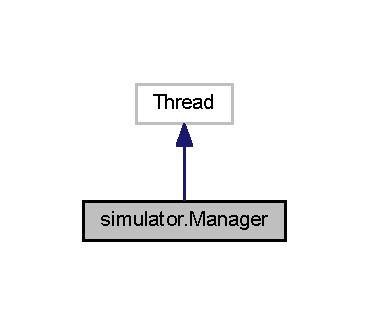
\includegraphics[width=177pt]{classsimulator_1_1_manager__inherit__graph}
\end{center}
\end{figure}


Collaboration diagram for simulator.\+Manager\+:\nopagebreak
\begin{figure}[H]
\begin{center}
\leavevmode
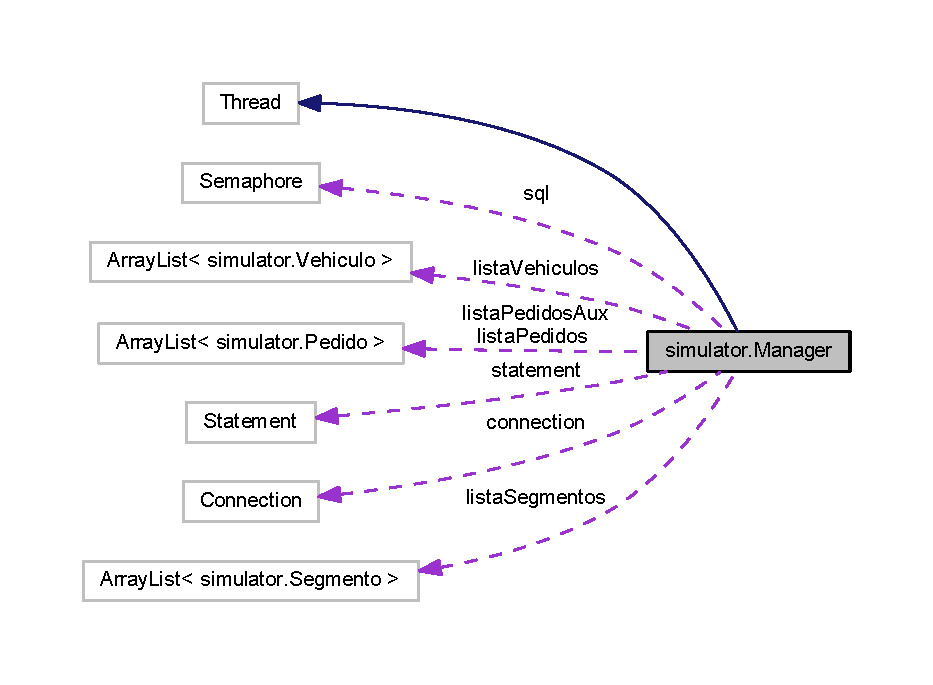
\includegraphics[width=350pt]{classsimulator_1_1_manager__coll__graph}
\end{center}
\end{figure}
\subsection*{Public Member Functions}
\begin{DoxyCompactItemize}
\item 
\mbox{\hyperlink{classsimulator_1_1_manager_af97cb12adc0ee7caa9e83f73ee85c04a}{Manager}} (Array\+List$<$ \mbox{\hyperlink{classsimulator_1_1_vehiculo}{Vehiculo}} $>$ lista\+Vehiculos, Semaphore sql, Array\+List$<$ \mbox{\hyperlink{classsimulator_1_1_segmento}{Segmento}} $>$ lista\+Segmentos)
\item 
void \mbox{\hyperlink{classsimulator_1_1_manager_adba6b4255dbc64064c6577e4baadbe9a}{connect}} (String username)
\item 
void \mbox{\hyperlink{classsimulator_1_1_manager_af238d6fc1282f769de925bf6aa9cdca9}{disconnect}} ()
\item 
void \mbox{\hyperlink{classsimulator_1_1_manager_a92b9df5fb7f406bfe8f99cdb8b6ee22a}{entregar}} (int pedido\+ID, int producto\+ID)
\item 
void \mbox{\hyperlink{classsimulator_1_1_manager_a318010c8020487c27cc127fdfe75402a}{leer\+Database}} ()
\item 
void \mbox{\hyperlink{classsimulator_1_1_manager_a6c22bed4ba7b715b4a4c0326ffd1f8a1}{asignar}} ()
\item 
void \mbox{\hyperlink{classsimulator_1_1_manager_ad98ac45d17514772c17a9c65be7d3892}{run}} ()
\item 
Array\+List$<$ \mbox{\hyperlink{classsimulator_1_1_vehiculo}{Vehiculo}} $>$ \mbox{\hyperlink{classsimulator_1_1_manager_a55b039767305793c0b904b49fe41cd56}{get\+Lista\+Vehiculos}} ()
\item 
void \mbox{\hyperlink{classsimulator_1_1_manager_a8f54c75ba31adb082ffbf25813caad71}{set\+Lista\+Vehiculos}} (Array\+List$<$ \mbox{\hyperlink{classsimulator_1_1_vehiculo}{Vehiculo}} $>$ lista\+Vehiculos)
\item 
Array\+List$<$ \mbox{\hyperlink{classsimulator_1_1_segmento}{Segmento}} $>$ \mbox{\hyperlink{classsimulator_1_1_manager_a8d708b20d559aa8fd42c9f963f2dc6d4}{get\+Lista\+Segmentos}} ()
\item 
void \mbox{\hyperlink{classsimulator_1_1_manager_af491f7a126893a6436bbd624ffc17ed9}{set\+Lista\+Segmentos}} (Array\+List$<$ \mbox{\hyperlink{classsimulator_1_1_segmento}{Segmento}} $>$ lista\+Segmentos)
\item 
Connection \mbox{\hyperlink{classsimulator_1_1_manager_a2a8f351e284baaf0b7ecd92dbf71468b}{get\+Connection}} ()
\item 
void \mbox{\hyperlink{classsimulator_1_1_manager_adc747823ff8f856a79a78a30ae6788f9}{set\+Connection}} (Connection connection)
\item 
Statement \mbox{\hyperlink{classsimulator_1_1_manager_ad753f8ec42bb1b7a2d5c3b0a5ff7ed99}{get\+Statement}} ()
\item 
void \mbox{\hyperlink{classsimulator_1_1_manager_ab4d473d9764b3aab34e02cc10a1e9645}{set\+Statement}} (Statement statement)
\item 
String \mbox{\hyperlink{classsimulator_1_1_manager_a74a372ec99052be3ceced43baeedbeac}{get\+Check}} ()
\item 
void \mbox{\hyperlink{classsimulator_1_1_manager_aaaf1f38ecbe1e8d2ca7ad20081ab378a}{set\+Check}} (String check)
\item 
Array\+List$<$ \mbox{\hyperlink{classsimulator_1_1_pedido}{Pedido}} $>$ \mbox{\hyperlink{classsimulator_1_1_manager_a98f04170b85509ae8f1fe2753dac60ef}{get\+Lista\+Pedidos}} ()
\item 
void \mbox{\hyperlink{classsimulator_1_1_manager_a3ac3fa3e9c1e559bbd50df24fe32fe33}{set\+Lista\+Pedidos}} (Array\+List$<$ \mbox{\hyperlink{classsimulator_1_1_pedido}{Pedido}} $>$ lista\+Pedidos)
\item 
Array\+List$<$ \mbox{\hyperlink{classsimulator_1_1_pedido}{Pedido}} $>$ \mbox{\hyperlink{classsimulator_1_1_manager_af266ad72ad536f9e58a75a3d070228cf}{get\+Lista\+Pedidos\+Aux}} ()
\item 
void \mbox{\hyperlink{classsimulator_1_1_manager_aa41c5e11ec1083566137aa868fea0049}{set\+Lista\+Pedidos\+Aux}} (Array\+List$<$ \mbox{\hyperlink{classsimulator_1_1_pedido}{Pedido}} $>$ lista\+Pedidos\+Aux)
\end{DoxyCompactItemize}


\subsection{Detailed Description}
This is the object M\+A\+N\+A\+G\+ER that has the methods to do the conection and disconection for the database.

\begin{DoxyAuthor}{Author}
Joseba Carnicero, Aitor Eizmendi, Jon Mugica and Marcos Azkarate 
\end{DoxyAuthor}


Definition at line 20 of file Manager.\+java.



\subsection{Constructor \& Destructor Documentation}
\mbox{\Hypertarget{classsimulator_1_1_manager_af97cb12adc0ee7caa9e83f73ee85c04a}\label{classsimulator_1_1_manager_af97cb12adc0ee7caa9e83f73ee85c04a}} 
\index{simulator\+::\+Manager@{simulator\+::\+Manager}!Manager@{Manager}}
\index{Manager@{Manager}!simulator\+::\+Manager@{simulator\+::\+Manager}}
\subsubsection{\texorpdfstring{Manager()}{Manager()}}
{\footnotesize\ttfamily simulator.\+Manager.\+Manager (\begin{DoxyParamCaption}\item[{Array\+List$<$ \mbox{\hyperlink{classsimulator_1_1_vehiculo}{Vehiculo}} $>$}]{lista\+Vehiculos,  }\item[{Semaphore}]{sql,  }\item[{Array\+List$<$ \mbox{\hyperlink{classsimulator_1_1_segmento}{Segmento}} $>$}]{lista\+Segmentos }\end{DoxyParamCaption})}

Parameterized constructor.


\begin{DoxyParams}{Parameters}
{\em lista\+Vehiculos} & contains an Array\+List of Vehicles \\
\hline
{\em sql} & is a Semaphore that it is used to a good synchronization \\
\hline
{\em lista\+Segmentos} & is an Array\+List of Segments \\
\hline
\end{DoxyParams}


Definition at line 50 of file Manager.\+java.

Here is the call graph for this function\+:\nopagebreak
\begin{figure}[H]
\begin{center}
\leavevmode
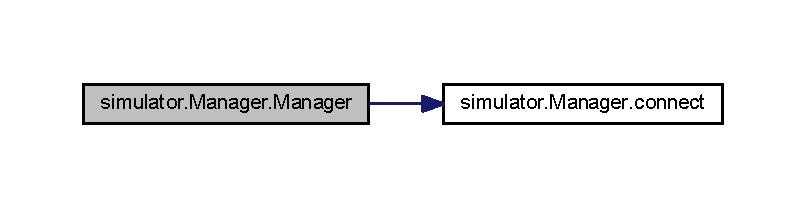
\includegraphics[width=350pt]{classsimulator_1_1_manager_af97cb12adc0ee7caa9e83f73ee85c04a_cgraph}
\end{center}
\end{figure}


\subsection{Member Function Documentation}
\mbox{\Hypertarget{classsimulator_1_1_manager_a6c22bed4ba7b715b4a4c0326ffd1f8a1}\label{classsimulator_1_1_manager_a6c22bed4ba7b715b4a4c0326ffd1f8a1}} 
\index{simulator\+::\+Manager@{simulator\+::\+Manager}!asignar@{asignar}}
\index{asignar@{asignar}!simulator\+::\+Manager@{simulator\+::\+Manager}}
\subsubsection{\texorpdfstring{asignar()}{asignar()}}
{\footnotesize\ttfamily void simulator.\+Manager.\+asignar (\begin{DoxyParamCaption}{ }\end{DoxyParamCaption})}

This method assigned different segment according to its priority 

Definition at line 208 of file Manager.\+java.

\mbox{\Hypertarget{classsimulator_1_1_manager_adba6b4255dbc64064c6577e4baadbe9a}\label{classsimulator_1_1_manager_adba6b4255dbc64064c6577e4baadbe9a}} 
\index{simulator\+::\+Manager@{simulator\+::\+Manager}!connect@{connect}}
\index{connect@{connect}!simulator\+::\+Manager@{simulator\+::\+Manager}}
\subsubsection{\texorpdfstring{connect()}{connect()}}
{\footnotesize\ttfamily void simulator.\+Manager.\+connect (\begin{DoxyParamCaption}\item[{String}]{username }\end{DoxyParamCaption})}

This method connects to the selected database 

Definition at line 61 of file Manager.\+java.

\mbox{\Hypertarget{classsimulator_1_1_manager_af238d6fc1282f769de925bf6aa9cdca9}\label{classsimulator_1_1_manager_af238d6fc1282f769de925bf6aa9cdca9}} 
\index{simulator\+::\+Manager@{simulator\+::\+Manager}!disconnect@{disconnect}}
\index{disconnect@{disconnect}!simulator\+::\+Manager@{simulator\+::\+Manager}}
\subsubsection{\texorpdfstring{disconnect()}{disconnect()}}
{\footnotesize\ttfamily void simulator.\+Manager.\+disconnect (\begin{DoxyParamCaption}{ }\end{DoxyParamCaption})}

This method closes the connected to the selected database 

Definition at line 84 of file Manager.\+java.

\mbox{\Hypertarget{classsimulator_1_1_manager_a92b9df5fb7f406bfe8f99cdb8b6ee22a}\label{classsimulator_1_1_manager_a92b9df5fb7f406bfe8f99cdb8b6ee22a}} 
\index{simulator\+::\+Manager@{simulator\+::\+Manager}!entregar@{entregar}}
\index{entregar@{entregar}!simulator\+::\+Manager@{simulator\+::\+Manager}}
\subsubsection{\texorpdfstring{entregar()}{entregar()}}
{\footnotesize\ttfamily void simulator.\+Manager.\+entregar (\begin{DoxyParamCaption}\item[{int}]{pedido\+ID,  }\item[{int}]{producto\+ID }\end{DoxyParamCaption})}

Parameterized constructor.


\begin{DoxyParams}{Parameters}
{\em int} & pedido\+ID describes the Id a certain order has \\
\hline
{\em int} & producto\+ID describes the Id a certain product has\\
\hline
\end{DoxyParams}
This method delivers all the products of a new order and change the status of the order into \char`\"{}\+Finished\char`\"{} 

Definition at line 114 of file Manager.\+java.

\mbox{\Hypertarget{classsimulator_1_1_manager_a74a372ec99052be3ceced43baeedbeac}\label{classsimulator_1_1_manager_a74a372ec99052be3ceced43baeedbeac}} 
\index{simulator\+::\+Manager@{simulator\+::\+Manager}!get\+Check@{get\+Check}}
\index{get\+Check@{get\+Check}!simulator\+::\+Manager@{simulator\+::\+Manager}}
\subsubsection{\texorpdfstring{get\+Check()}{getCheck()}}
{\footnotesize\ttfamily String simulator.\+Manager.\+get\+Check (\begin{DoxyParamCaption}{ }\end{DoxyParamCaption})}



Definition at line 341 of file Manager.\+java.

\mbox{\Hypertarget{classsimulator_1_1_manager_a2a8f351e284baaf0b7ecd92dbf71468b}\label{classsimulator_1_1_manager_a2a8f351e284baaf0b7ecd92dbf71468b}} 
\index{simulator\+::\+Manager@{simulator\+::\+Manager}!get\+Connection@{get\+Connection}}
\index{get\+Connection@{get\+Connection}!simulator\+::\+Manager@{simulator\+::\+Manager}}
\subsubsection{\texorpdfstring{get\+Connection()}{getConnection()}}
{\footnotesize\ttfamily Connection simulator.\+Manager.\+get\+Connection (\begin{DoxyParamCaption}{ }\end{DoxyParamCaption})}



Definition at line 325 of file Manager.\+java.

\mbox{\Hypertarget{classsimulator_1_1_manager_a98f04170b85509ae8f1fe2753dac60ef}\label{classsimulator_1_1_manager_a98f04170b85509ae8f1fe2753dac60ef}} 
\index{simulator\+::\+Manager@{simulator\+::\+Manager}!get\+Lista\+Pedidos@{get\+Lista\+Pedidos}}
\index{get\+Lista\+Pedidos@{get\+Lista\+Pedidos}!simulator\+::\+Manager@{simulator\+::\+Manager}}
\subsubsection{\texorpdfstring{get\+Lista\+Pedidos()}{getListaPedidos()}}
{\footnotesize\ttfamily Array\+List$<$\mbox{\hyperlink{classsimulator_1_1_pedido}{Pedido}}$>$ simulator.\+Manager.\+get\+Lista\+Pedidos (\begin{DoxyParamCaption}{ }\end{DoxyParamCaption})}



Definition at line 349 of file Manager.\+java.

\mbox{\Hypertarget{classsimulator_1_1_manager_af266ad72ad536f9e58a75a3d070228cf}\label{classsimulator_1_1_manager_af266ad72ad536f9e58a75a3d070228cf}} 
\index{simulator\+::\+Manager@{simulator\+::\+Manager}!get\+Lista\+Pedidos\+Aux@{get\+Lista\+Pedidos\+Aux}}
\index{get\+Lista\+Pedidos\+Aux@{get\+Lista\+Pedidos\+Aux}!simulator\+::\+Manager@{simulator\+::\+Manager}}
\subsubsection{\texorpdfstring{get\+Lista\+Pedidos\+Aux()}{getListaPedidosAux()}}
{\footnotesize\ttfamily Array\+List$<$\mbox{\hyperlink{classsimulator_1_1_pedido}{Pedido}}$>$ simulator.\+Manager.\+get\+Lista\+Pedidos\+Aux (\begin{DoxyParamCaption}{ }\end{DoxyParamCaption})}



Definition at line 357 of file Manager.\+java.

\mbox{\Hypertarget{classsimulator_1_1_manager_a8d708b20d559aa8fd42c9f963f2dc6d4}\label{classsimulator_1_1_manager_a8d708b20d559aa8fd42c9f963f2dc6d4}} 
\index{simulator\+::\+Manager@{simulator\+::\+Manager}!get\+Lista\+Segmentos@{get\+Lista\+Segmentos}}
\index{get\+Lista\+Segmentos@{get\+Lista\+Segmentos}!simulator\+::\+Manager@{simulator\+::\+Manager}}
\subsubsection{\texorpdfstring{get\+Lista\+Segmentos()}{getListaSegmentos()}}
{\footnotesize\ttfamily Array\+List$<$\mbox{\hyperlink{classsimulator_1_1_segmento}{Segmento}}$>$ simulator.\+Manager.\+get\+Lista\+Segmentos (\begin{DoxyParamCaption}{ }\end{DoxyParamCaption})}



Definition at line 317 of file Manager.\+java.

\mbox{\Hypertarget{classsimulator_1_1_manager_a55b039767305793c0b904b49fe41cd56}\label{classsimulator_1_1_manager_a55b039767305793c0b904b49fe41cd56}} 
\index{simulator\+::\+Manager@{simulator\+::\+Manager}!get\+Lista\+Vehiculos@{get\+Lista\+Vehiculos}}
\index{get\+Lista\+Vehiculos@{get\+Lista\+Vehiculos}!simulator\+::\+Manager@{simulator\+::\+Manager}}
\subsubsection{\texorpdfstring{get\+Lista\+Vehiculos()}{getListaVehiculos()}}
{\footnotesize\ttfamily Array\+List$<$\mbox{\hyperlink{classsimulator_1_1_vehiculo}{Vehiculo}}$>$ simulator.\+Manager.\+get\+Lista\+Vehiculos (\begin{DoxyParamCaption}{ }\end{DoxyParamCaption})}



Definition at line 309 of file Manager.\+java.

\mbox{\Hypertarget{classsimulator_1_1_manager_ad753f8ec42bb1b7a2d5c3b0a5ff7ed99}\label{classsimulator_1_1_manager_ad753f8ec42bb1b7a2d5c3b0a5ff7ed99}} 
\index{simulator\+::\+Manager@{simulator\+::\+Manager}!get\+Statement@{get\+Statement}}
\index{get\+Statement@{get\+Statement}!simulator\+::\+Manager@{simulator\+::\+Manager}}
\subsubsection{\texorpdfstring{get\+Statement()}{getStatement()}}
{\footnotesize\ttfamily Statement simulator.\+Manager.\+get\+Statement (\begin{DoxyParamCaption}{ }\end{DoxyParamCaption})}



Definition at line 333 of file Manager.\+java.

\mbox{\Hypertarget{classsimulator_1_1_manager_a318010c8020487c27cc127fdfe75402a}\label{classsimulator_1_1_manager_a318010c8020487c27cc127fdfe75402a}} 
\index{simulator\+::\+Manager@{simulator\+::\+Manager}!leer\+Database@{leer\+Database}}
\index{leer\+Database@{leer\+Database}!simulator\+::\+Manager@{simulator\+::\+Manager}}
\subsubsection{\texorpdfstring{leer\+Database()}{leerDatabase()}}
{\footnotesize\ttfamily void simulator.\+Manager.\+leer\+Database (\begin{DoxyParamCaption}{ }\end{DoxyParamCaption})}

This method reads from the database the new orders and 

Definition at line 155 of file Manager.\+java.

\mbox{\Hypertarget{classsimulator_1_1_manager_ad98ac45d17514772c17a9c65be7d3892}\label{classsimulator_1_1_manager_ad98ac45d17514772c17a9c65be7d3892}} 
\index{simulator\+::\+Manager@{simulator\+::\+Manager}!run@{run}}
\index{run@{run}!simulator\+::\+Manager@{simulator\+::\+Manager}}
\subsubsection{\texorpdfstring{run()}{run()}}
{\footnotesize\ttfamily void simulator.\+Manager.\+run (\begin{DoxyParamCaption}{ }\end{DoxyParamCaption})}

This method display the actual position of the autonomous vehicles and the status of the different workstations 

Definition at line 282 of file Manager.\+java.

Here is the call graph for this function\+:\nopagebreak
\begin{figure}[H]
\begin{center}
\leavevmode
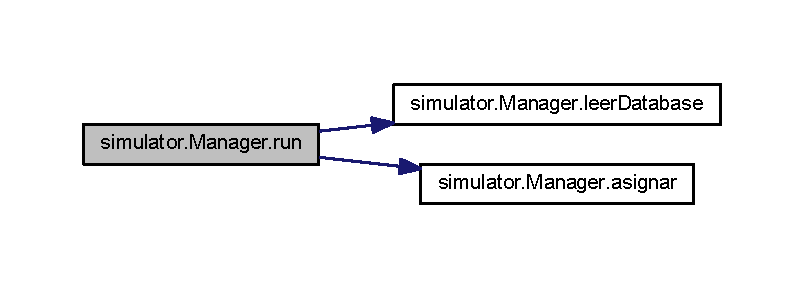
\includegraphics[width=350pt]{classsimulator_1_1_manager_ad98ac45d17514772c17a9c65be7d3892_cgraph}
\end{center}
\end{figure}
\mbox{\Hypertarget{classsimulator_1_1_manager_aaaf1f38ecbe1e8d2ca7ad20081ab378a}\label{classsimulator_1_1_manager_aaaf1f38ecbe1e8d2ca7ad20081ab378a}} 
\index{simulator\+::\+Manager@{simulator\+::\+Manager}!set\+Check@{set\+Check}}
\index{set\+Check@{set\+Check}!simulator\+::\+Manager@{simulator\+::\+Manager}}
\subsubsection{\texorpdfstring{set\+Check()}{setCheck()}}
{\footnotesize\ttfamily void simulator.\+Manager.\+set\+Check (\begin{DoxyParamCaption}\item[{String}]{check }\end{DoxyParamCaption})}



Definition at line 345 of file Manager.\+java.

\mbox{\Hypertarget{classsimulator_1_1_manager_adc747823ff8f856a79a78a30ae6788f9}\label{classsimulator_1_1_manager_adc747823ff8f856a79a78a30ae6788f9}} 
\index{simulator\+::\+Manager@{simulator\+::\+Manager}!set\+Connection@{set\+Connection}}
\index{set\+Connection@{set\+Connection}!simulator\+::\+Manager@{simulator\+::\+Manager}}
\subsubsection{\texorpdfstring{set\+Connection()}{setConnection()}}
{\footnotesize\ttfamily void simulator.\+Manager.\+set\+Connection (\begin{DoxyParamCaption}\item[{Connection}]{connection }\end{DoxyParamCaption})}



Definition at line 329 of file Manager.\+java.

\mbox{\Hypertarget{classsimulator_1_1_manager_a3ac3fa3e9c1e559bbd50df24fe32fe33}\label{classsimulator_1_1_manager_a3ac3fa3e9c1e559bbd50df24fe32fe33}} 
\index{simulator\+::\+Manager@{simulator\+::\+Manager}!set\+Lista\+Pedidos@{set\+Lista\+Pedidos}}
\index{set\+Lista\+Pedidos@{set\+Lista\+Pedidos}!simulator\+::\+Manager@{simulator\+::\+Manager}}
\subsubsection{\texorpdfstring{set\+Lista\+Pedidos()}{setListaPedidos()}}
{\footnotesize\ttfamily void simulator.\+Manager.\+set\+Lista\+Pedidos (\begin{DoxyParamCaption}\item[{Array\+List$<$ \mbox{\hyperlink{classsimulator_1_1_pedido}{Pedido}} $>$}]{lista\+Pedidos }\end{DoxyParamCaption})}



Definition at line 353 of file Manager.\+java.

\mbox{\Hypertarget{classsimulator_1_1_manager_aa41c5e11ec1083566137aa868fea0049}\label{classsimulator_1_1_manager_aa41c5e11ec1083566137aa868fea0049}} 
\index{simulator\+::\+Manager@{simulator\+::\+Manager}!set\+Lista\+Pedidos\+Aux@{set\+Lista\+Pedidos\+Aux}}
\index{set\+Lista\+Pedidos\+Aux@{set\+Lista\+Pedidos\+Aux}!simulator\+::\+Manager@{simulator\+::\+Manager}}
\subsubsection{\texorpdfstring{set\+Lista\+Pedidos\+Aux()}{setListaPedidosAux()}}
{\footnotesize\ttfamily void simulator.\+Manager.\+set\+Lista\+Pedidos\+Aux (\begin{DoxyParamCaption}\item[{Array\+List$<$ \mbox{\hyperlink{classsimulator_1_1_pedido}{Pedido}} $>$}]{lista\+Pedidos\+Aux }\end{DoxyParamCaption})}



Definition at line 361 of file Manager.\+java.

\mbox{\Hypertarget{classsimulator_1_1_manager_af491f7a126893a6436bbd624ffc17ed9}\label{classsimulator_1_1_manager_af491f7a126893a6436bbd624ffc17ed9}} 
\index{simulator\+::\+Manager@{simulator\+::\+Manager}!set\+Lista\+Segmentos@{set\+Lista\+Segmentos}}
\index{set\+Lista\+Segmentos@{set\+Lista\+Segmentos}!simulator\+::\+Manager@{simulator\+::\+Manager}}
\subsubsection{\texorpdfstring{set\+Lista\+Segmentos()}{setListaSegmentos()}}
{\footnotesize\ttfamily void simulator.\+Manager.\+set\+Lista\+Segmentos (\begin{DoxyParamCaption}\item[{Array\+List$<$ \mbox{\hyperlink{classsimulator_1_1_segmento}{Segmento}} $>$}]{lista\+Segmentos }\end{DoxyParamCaption})}



Definition at line 321 of file Manager.\+java.

\mbox{\Hypertarget{classsimulator_1_1_manager_a8f54c75ba31adb082ffbf25813caad71}\label{classsimulator_1_1_manager_a8f54c75ba31adb082ffbf25813caad71}} 
\index{simulator\+::\+Manager@{simulator\+::\+Manager}!set\+Lista\+Vehiculos@{set\+Lista\+Vehiculos}}
\index{set\+Lista\+Vehiculos@{set\+Lista\+Vehiculos}!simulator\+::\+Manager@{simulator\+::\+Manager}}
\subsubsection{\texorpdfstring{set\+Lista\+Vehiculos()}{setListaVehiculos()}}
{\footnotesize\ttfamily void simulator.\+Manager.\+set\+Lista\+Vehiculos (\begin{DoxyParamCaption}\item[{Array\+List$<$ \mbox{\hyperlink{classsimulator_1_1_vehiculo}{Vehiculo}} $>$}]{lista\+Vehiculos }\end{DoxyParamCaption})}



Definition at line 313 of file Manager.\+java.

\mbox{\Hypertarget{classsimulator_1_1_manager_ab4d473d9764b3aab34e02cc10a1e9645}\label{classsimulator_1_1_manager_ab4d473d9764b3aab34e02cc10a1e9645}} 
\index{simulator\+::\+Manager@{simulator\+::\+Manager}!set\+Statement@{set\+Statement}}
\index{set\+Statement@{set\+Statement}!simulator\+::\+Manager@{simulator\+::\+Manager}}
\subsubsection{\texorpdfstring{set\+Statement()}{setStatement()}}
{\footnotesize\ttfamily void simulator.\+Manager.\+set\+Statement (\begin{DoxyParamCaption}\item[{Statement}]{statement }\end{DoxyParamCaption})}



Definition at line 337 of file Manager.\+java.



The documentation for this class was generated from the following file\+:\begin{DoxyCompactItemize}
\item 
java/main/java/simulator/\mbox{\hyperlink{_manager_8java}{Manager.\+java}}\end{DoxyCompactItemize}

\hypertarget{classtest_1_1_manager_test}{}\section{test.\+Manager\+Test Class Reference}
\label{classtest_1_1_manager_test}\index{test.\+Manager\+Test@{test.\+Manager\+Test}}


Collaboration diagram for test.\+Manager\+Test\+:\nopagebreak
\begin{figure}[H]
\begin{center}
\leavevmode
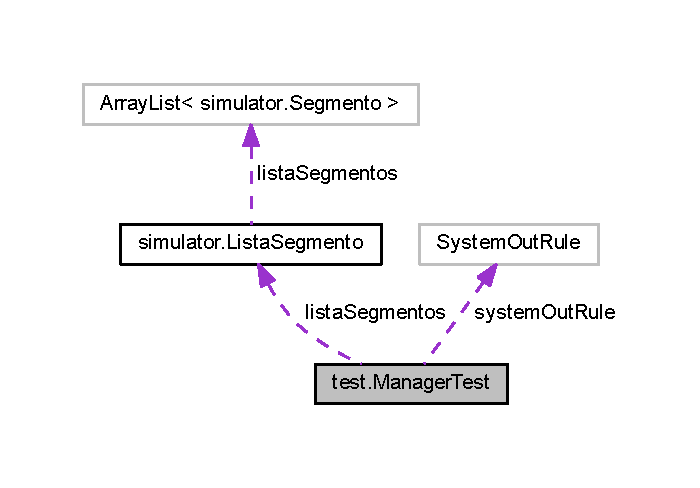
\includegraphics[width=336pt]{classtest_1_1_manager_test__coll__graph}
\end{center}
\end{figure}
\subsection*{Public Member Functions}
\begin{DoxyCompactItemize}
\item 
void \mbox{\hyperlink{classtest_1_1_manager_test_ad710f9a15cc2d2f6aaeb827b25cbd1d2}{before}} ()
\item 
void \mbox{\hyperlink{classtest_1_1_manager_test_a7b2f9075ed25eb6389bb263099a75c1c}{connect\+Test}} ()
\item 
void \mbox{\hyperlink{classtest_1_1_manager_test_a85a4be4f4bd5606a127e983fa4e3883d}{Class\+Not\+Found\+Exception\+Test}} ()  throws S\+Q\+L\+Exception
\item 
void \mbox{\hyperlink{classtest_1_1_manager_test_af4a31042b6841a262fa71d6da2c24279}{disconnect\+Test}} ()
\item 
void \mbox{\hyperlink{classtest_1_1_manager_test_ac84a6778c74c43fc017ab5297f94584e}{leer\+Database\+Test}} ()
\item 
void \mbox{\hyperlink{classtest_1_1_manager_test_a38faaaeb2a9599c4efdc76b6d7b36a96}{entregar\+Test}} ()
\item 
void \mbox{\hyperlink{classtest_1_1_manager_test_ab470b5d3e7f291fa187e1c737d782b34}{asignar\+Test}} ()
\end{DoxyCompactItemize}
\subsection*{Public Attributes}
\begin{DoxyCompactItemize}
\item 
final System\+Out\+Rule \mbox{\hyperlink{classtest_1_1_manager_test_a145ff3d1782752daa94a07ab9c2cb312}{system\+Out\+Rule}} = new System\+Out\+Rule().enable\+Log()
\end{DoxyCompactItemize}


\subsection{Detailed Description}


Definition at line 22 of file Manager\+Test.\+java.



\subsection{Member Function Documentation}
\mbox{\Hypertarget{classtest_1_1_manager_test_ab470b5d3e7f291fa187e1c737d782b34}\label{classtest_1_1_manager_test_ab470b5d3e7f291fa187e1c737d782b34}} 
\index{test\+::\+Manager\+Test@{test\+::\+Manager\+Test}!asignar\+Test@{asignar\+Test}}
\index{asignar\+Test@{asignar\+Test}!test\+::\+Manager\+Test@{test\+::\+Manager\+Test}}
\subsubsection{\texorpdfstring{asignar\+Test()}{asignarTest()}}
{\footnotesize\ttfamily void test.\+Manager\+Test.\+asignar\+Test (\begin{DoxyParamCaption}{ }\end{DoxyParamCaption})}



Definition at line 111 of file Manager\+Test.\+java.

Here is the call graph for this function\+:\nopagebreak
\begin{figure}[H]
\begin{center}
\leavevmode
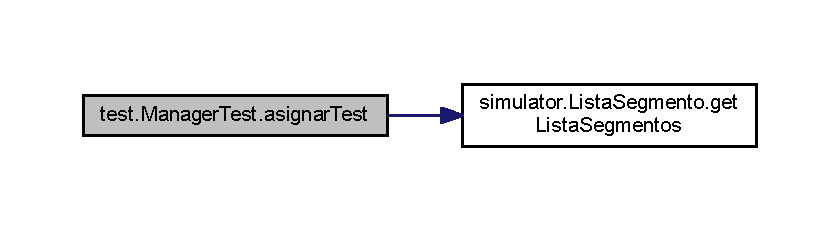
\includegraphics[width=350pt]{classtest_1_1_manager_test_ab470b5d3e7f291fa187e1c737d782b34_cgraph}
\end{center}
\end{figure}
\mbox{\Hypertarget{classtest_1_1_manager_test_ad710f9a15cc2d2f6aaeb827b25cbd1d2}\label{classtest_1_1_manager_test_ad710f9a15cc2d2f6aaeb827b25cbd1d2}} 
\index{test\+::\+Manager\+Test@{test\+::\+Manager\+Test}!before@{before}}
\index{before@{before}!test\+::\+Manager\+Test@{test\+::\+Manager\+Test}}
\subsubsection{\texorpdfstring{before()}{before()}}
{\footnotesize\ttfamily void test.\+Manager\+Test.\+before (\begin{DoxyParamCaption}{ }\end{DoxyParamCaption})}



Definition at line 30 of file Manager\+Test.\+java.

Here is the call graph for this function\+:\nopagebreak
\begin{figure}[H]
\begin{center}
\leavevmode
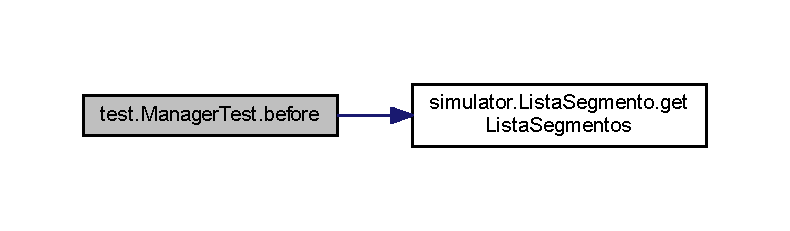
\includegraphics[width=350pt]{classtest_1_1_manager_test_ad710f9a15cc2d2f6aaeb827b25cbd1d2_cgraph}
\end{center}
\end{figure}
\mbox{\Hypertarget{classtest_1_1_manager_test_a85a4be4f4bd5606a127e983fa4e3883d}\label{classtest_1_1_manager_test_a85a4be4f4bd5606a127e983fa4e3883d}} 
\index{test\+::\+Manager\+Test@{test\+::\+Manager\+Test}!Class\+Not\+Found\+Exception\+Test@{Class\+Not\+Found\+Exception\+Test}}
\index{Class\+Not\+Found\+Exception\+Test@{Class\+Not\+Found\+Exception\+Test}!test\+::\+Manager\+Test@{test\+::\+Manager\+Test}}
\subsubsection{\texorpdfstring{Class\+Not\+Found\+Exception\+Test()}{ClassNotFoundExceptionTest()}}
{\footnotesize\ttfamily void test.\+Manager\+Test.\+Class\+Not\+Found\+Exception\+Test (\begin{DoxyParamCaption}{ }\end{DoxyParamCaption}) throws S\+Q\+L\+Exception}



Definition at line 49 of file Manager\+Test.\+java.

\mbox{\Hypertarget{classtest_1_1_manager_test_a7b2f9075ed25eb6389bb263099a75c1c}\label{classtest_1_1_manager_test_a7b2f9075ed25eb6389bb263099a75c1c}} 
\index{test\+::\+Manager\+Test@{test\+::\+Manager\+Test}!connect\+Test@{connect\+Test}}
\index{connect\+Test@{connect\+Test}!test\+::\+Manager\+Test@{test\+::\+Manager\+Test}}
\subsubsection{\texorpdfstring{connect\+Test()}{connectTest()}}
{\footnotesize\ttfamily void test.\+Manager\+Test.\+connect\+Test (\begin{DoxyParamCaption}{ }\end{DoxyParamCaption})}



Definition at line 42 of file Manager\+Test.\+java.

\mbox{\Hypertarget{classtest_1_1_manager_test_af4a31042b6841a262fa71d6da2c24279}\label{classtest_1_1_manager_test_af4a31042b6841a262fa71d6da2c24279}} 
\index{test\+::\+Manager\+Test@{test\+::\+Manager\+Test}!disconnect\+Test@{disconnect\+Test}}
\index{disconnect\+Test@{disconnect\+Test}!test\+::\+Manager\+Test@{test\+::\+Manager\+Test}}
\subsubsection{\texorpdfstring{disconnect\+Test()}{disconnectTest()}}
{\footnotesize\ttfamily void test.\+Manager\+Test.\+disconnect\+Test (\begin{DoxyParamCaption}{ }\end{DoxyParamCaption})}



Definition at line 61 of file Manager\+Test.\+java.

\mbox{\Hypertarget{classtest_1_1_manager_test_a38faaaeb2a9599c4efdc76b6d7b36a96}\label{classtest_1_1_manager_test_a38faaaeb2a9599c4efdc76b6d7b36a96}} 
\index{test\+::\+Manager\+Test@{test\+::\+Manager\+Test}!entregar\+Test@{entregar\+Test}}
\index{entregar\+Test@{entregar\+Test}!test\+::\+Manager\+Test@{test\+::\+Manager\+Test}}
\subsubsection{\texorpdfstring{entregar\+Test()}{entregarTest()}}
{\footnotesize\ttfamily void test.\+Manager\+Test.\+entregar\+Test (\begin{DoxyParamCaption}{ }\end{DoxyParamCaption})}



Definition at line 91 of file Manager\+Test.\+java.

\mbox{\Hypertarget{classtest_1_1_manager_test_ac84a6778c74c43fc017ab5297f94584e}\label{classtest_1_1_manager_test_ac84a6778c74c43fc017ab5297f94584e}} 
\index{test\+::\+Manager\+Test@{test\+::\+Manager\+Test}!leer\+Database\+Test@{leer\+Database\+Test}}
\index{leer\+Database\+Test@{leer\+Database\+Test}!test\+::\+Manager\+Test@{test\+::\+Manager\+Test}}
\subsubsection{\texorpdfstring{leer\+Database\+Test()}{leerDatabaseTest()}}
{\footnotesize\ttfamily void test.\+Manager\+Test.\+leer\+Database\+Test (\begin{DoxyParamCaption}{ }\end{DoxyParamCaption})}



Definition at line 73 of file Manager\+Test.\+java.



\subsection{Member Data Documentation}
\mbox{\Hypertarget{classtest_1_1_manager_test_a145ff3d1782752daa94a07ab9c2cb312}\label{classtest_1_1_manager_test_a145ff3d1782752daa94a07ab9c2cb312}} 
\index{test\+::\+Manager\+Test@{test\+::\+Manager\+Test}!system\+Out\+Rule@{system\+Out\+Rule}}
\index{system\+Out\+Rule@{system\+Out\+Rule}!test\+::\+Manager\+Test@{test\+::\+Manager\+Test}}
\subsubsection{\texorpdfstring{system\+Out\+Rule}{systemOutRule}}
{\footnotesize\ttfamily final System\+Out\+Rule test.\+Manager\+Test.\+system\+Out\+Rule = new System\+Out\+Rule().enable\+Log()}



Definition at line 39 of file Manager\+Test.\+java.



The documentation for this class was generated from the following file\+:\begin{DoxyCompactItemize}
\item 
java/test/java/test/\mbox{\hyperlink{_manager_test_8java}{Manager\+Test.\+java}}\end{DoxyCompactItemize}

\hypertarget{classsimulator_1_1_pedido}{}\section{simulator.\+Pedido Class Reference}
\label{classsimulator_1_1_pedido}\index{simulator.\+Pedido@{simulator.\+Pedido}}


Collaboration diagram for simulator.\+Pedido\+:\nopagebreak
\begin{figure}[H]
\begin{center}
\leavevmode
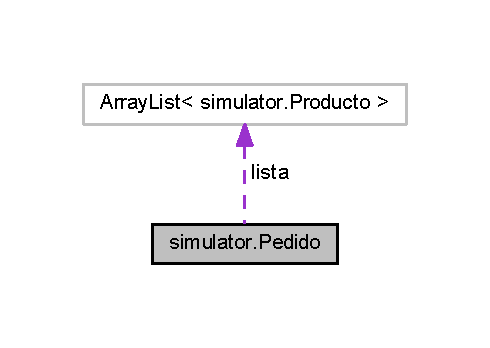
\includegraphics[width=235pt]{classsimulator_1_1_pedido__coll__graph}
\end{center}
\end{figure}
\subsection*{Public Member Functions}
\begin{DoxyCompactItemize}
\item 
\mbox{\hyperlink{classsimulator_1_1_pedido_a2587e6c91c06bfd2057039ff2e10874a}{Pedido}} (int id)
\item 
String \mbox{\hyperlink{classsimulator_1_1_pedido_a5519f7e51ab5b3506840f332a7cd1157}{to\+String}} ()
\item 
Array\+List$<$ \mbox{\hyperlink{classsimulator_1_1_producto}{Producto}} $>$ \mbox{\hyperlink{classsimulator_1_1_pedido_ae5b5f146669e6f891fc8dc8e58ef8c64}{get\+Lista}} ()
\item 
int \mbox{\hyperlink{classsimulator_1_1_pedido_a22c3691133eaa7c5b467072e2e4c3ed9}{get\+Id}} ()
\end{DoxyCompactItemize}


\subsection{Detailed Description}
This is the object \mbox{\hyperlink{classsimulator_1_1_pedido}{Pedido}} that has the paremeters id and a Array\+List

\begin{DoxyAuthor}{Author}
Joseba Carnicero, Aitor Eizmendi, Jon Mugica and Marcos Azkarate 
\end{DoxyAuthor}


Definition at line 10 of file Pedido.\+java.



\subsection{Constructor \& Destructor Documentation}
\mbox{\Hypertarget{classsimulator_1_1_pedido_a2587e6c91c06bfd2057039ff2e10874a}\label{classsimulator_1_1_pedido_a2587e6c91c06bfd2057039ff2e10874a}} 
\index{simulator\+::\+Pedido@{simulator\+::\+Pedido}!Pedido@{Pedido}}
\index{Pedido@{Pedido}!simulator\+::\+Pedido@{simulator\+::\+Pedido}}
\subsubsection{\texorpdfstring{Pedido()}{Pedido()}}
{\footnotesize\ttfamily simulator.\+Pedido.\+Pedido (\begin{DoxyParamCaption}\item[{int}]{id }\end{DoxyParamCaption})}



Definition at line 14 of file Pedido.\+java.



\subsection{Member Function Documentation}
\mbox{\Hypertarget{classsimulator_1_1_pedido_a22c3691133eaa7c5b467072e2e4c3ed9}\label{classsimulator_1_1_pedido_a22c3691133eaa7c5b467072e2e4c3ed9}} 
\index{simulator\+::\+Pedido@{simulator\+::\+Pedido}!get\+Id@{get\+Id}}
\index{get\+Id@{get\+Id}!simulator\+::\+Pedido@{simulator\+::\+Pedido}}
\subsubsection{\texorpdfstring{get\+Id()}{getId()}}
{\footnotesize\ttfamily int simulator.\+Pedido.\+get\+Id (\begin{DoxyParamCaption}{ }\end{DoxyParamCaption})}



Definition at line 28 of file Pedido.\+java.

\mbox{\Hypertarget{classsimulator_1_1_pedido_ae5b5f146669e6f891fc8dc8e58ef8c64}\label{classsimulator_1_1_pedido_ae5b5f146669e6f891fc8dc8e58ef8c64}} 
\index{simulator\+::\+Pedido@{simulator\+::\+Pedido}!get\+Lista@{get\+Lista}}
\index{get\+Lista@{get\+Lista}!simulator\+::\+Pedido@{simulator\+::\+Pedido}}
\subsubsection{\texorpdfstring{get\+Lista()}{getLista()}}
{\footnotesize\ttfamily Array\+List$<$\mbox{\hyperlink{classsimulator_1_1_producto}{Producto}}$>$ simulator.\+Pedido.\+get\+Lista (\begin{DoxyParamCaption}{ }\end{DoxyParamCaption})}



Definition at line 24 of file Pedido.\+java.

\mbox{\Hypertarget{classsimulator_1_1_pedido_a5519f7e51ab5b3506840f332a7cd1157}\label{classsimulator_1_1_pedido_a5519f7e51ab5b3506840f332a7cd1157}} 
\index{simulator\+::\+Pedido@{simulator\+::\+Pedido}!to\+String@{to\+String}}
\index{to\+String@{to\+String}!simulator\+::\+Pedido@{simulator\+::\+Pedido}}
\subsubsection{\texorpdfstring{to\+String()}{toString()}}
{\footnotesize\ttfamily String simulator.\+Pedido.\+to\+String (\begin{DoxyParamCaption}{ }\end{DoxyParamCaption})}



Definition at line 20 of file Pedido.\+java.



The documentation for this class was generated from the following file\+:\begin{DoxyCompactItemize}
\item 
java/main/java/simulator/\mbox{\hyperlink{_pedido_8java}{Pedido.\+java}}\end{DoxyCompactItemize}

\hypertarget{classtest_1_1_pedido_test}{}\section{test.\+Pedido\+Test Class Reference}
\label{classtest_1_1_pedido_test}\index{test.\+Pedido\+Test@{test.\+Pedido\+Test}}


Collaboration diagram for test.\+Pedido\+Test\+:\nopagebreak
\begin{figure}[H]
\begin{center}
\leavevmode
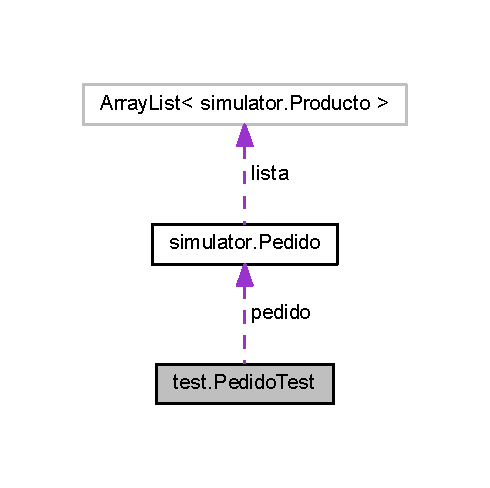
\includegraphics[width=235pt]{classtest_1_1_pedido_test__coll__graph}
\end{center}
\end{figure}
\subsection*{Public Member Functions}
\begin{DoxyCompactItemize}
\item 
void \mbox{\hyperlink{classtest_1_1_pedido_test_a224f87e09063855d190a6910ba42ce1a}{before}} ()
\item 
void \mbox{\hyperlink{classtest_1_1_pedido_test_a543df9133d7a9040b22b94c1d66dbf2b}{pedido\+Class}} ()
\item 
void \mbox{\hyperlink{classtest_1_1_pedido_test_a9e3efe0a23f91c6895ab6fe5da7621cb}{pedido\+To\+String}} ()
\item 
void \mbox{\hyperlink{classtest_1_1_pedido_test_a2685ac9664dc2e9bfba5d65b5b94bfbd}{pedido\+Lista}} ()
\end{DoxyCompactItemize}


\subsection{Detailed Description}


Definition at line 11 of file Pedido\+Test.\+java.



\subsection{Member Function Documentation}
\mbox{\Hypertarget{classtest_1_1_pedido_test_a224f87e09063855d190a6910ba42ce1a}\label{classtest_1_1_pedido_test_a224f87e09063855d190a6910ba42ce1a}} 
\index{test\+::\+Pedido\+Test@{test\+::\+Pedido\+Test}!before@{before}}
\index{before@{before}!test\+::\+Pedido\+Test@{test\+::\+Pedido\+Test}}
\subsubsection{\texorpdfstring{before()}{before()}}
{\footnotesize\ttfamily void test.\+Pedido\+Test.\+before (\begin{DoxyParamCaption}{ }\end{DoxyParamCaption})}



Definition at line 16 of file Pedido\+Test.\+java.

\mbox{\Hypertarget{classtest_1_1_pedido_test_a543df9133d7a9040b22b94c1d66dbf2b}\label{classtest_1_1_pedido_test_a543df9133d7a9040b22b94c1d66dbf2b}} 
\index{test\+::\+Pedido\+Test@{test\+::\+Pedido\+Test}!pedido\+Class@{pedido\+Class}}
\index{pedido\+Class@{pedido\+Class}!test\+::\+Pedido\+Test@{test\+::\+Pedido\+Test}}
\subsubsection{\texorpdfstring{pedido\+Class()}{pedidoClass()}}
{\footnotesize\ttfamily void test.\+Pedido\+Test.\+pedido\+Class (\begin{DoxyParamCaption}{ }\end{DoxyParamCaption})}



Definition at line 21 of file Pedido\+Test.\+java.

\mbox{\Hypertarget{classtest_1_1_pedido_test_a2685ac9664dc2e9bfba5d65b5b94bfbd}\label{classtest_1_1_pedido_test_a2685ac9664dc2e9bfba5d65b5b94bfbd}} 
\index{test\+::\+Pedido\+Test@{test\+::\+Pedido\+Test}!pedido\+Lista@{pedido\+Lista}}
\index{pedido\+Lista@{pedido\+Lista}!test\+::\+Pedido\+Test@{test\+::\+Pedido\+Test}}
\subsubsection{\texorpdfstring{pedido\+Lista()}{pedidoLista()}}
{\footnotesize\ttfamily void test.\+Pedido\+Test.\+pedido\+Lista (\begin{DoxyParamCaption}{ }\end{DoxyParamCaption})}



Definition at line 33 of file Pedido\+Test.\+java.

Here is the call graph for this function\+:\nopagebreak
\begin{figure}[H]
\begin{center}
\leavevmode
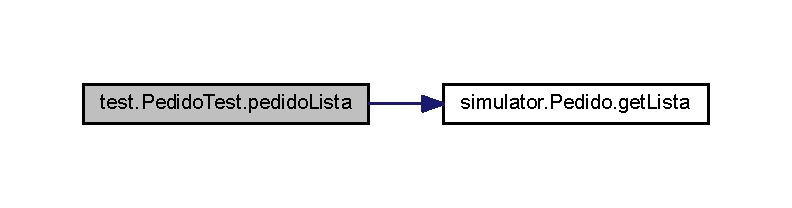
\includegraphics[width=350pt]{classtest_1_1_pedido_test_a2685ac9664dc2e9bfba5d65b5b94bfbd_cgraph}
\end{center}
\end{figure}
\mbox{\Hypertarget{classtest_1_1_pedido_test_a9e3efe0a23f91c6895ab6fe5da7621cb}\label{classtest_1_1_pedido_test_a9e3efe0a23f91c6895ab6fe5da7621cb}} 
\index{test\+::\+Pedido\+Test@{test\+::\+Pedido\+Test}!pedido\+To\+String@{pedido\+To\+String}}
\index{pedido\+To\+String@{pedido\+To\+String}!test\+::\+Pedido\+Test@{test\+::\+Pedido\+Test}}
\subsubsection{\texorpdfstring{pedido\+To\+String()}{pedidoToString()}}
{\footnotesize\ttfamily void test.\+Pedido\+Test.\+pedido\+To\+String (\begin{DoxyParamCaption}{ }\end{DoxyParamCaption})}



Definition at line 27 of file Pedido\+Test.\+java.

Here is the call graph for this function\+:\nopagebreak
\begin{figure}[H]
\begin{center}
\leavevmode
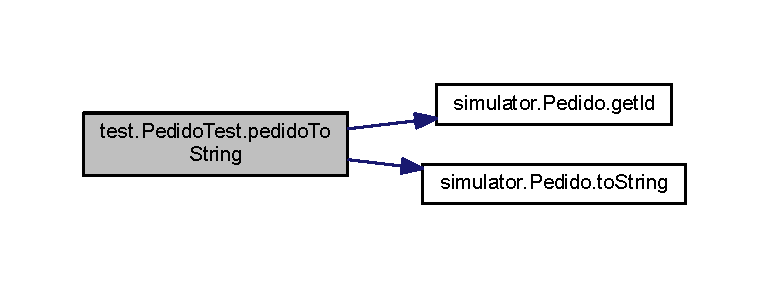
\includegraphics[width=350pt]{classtest_1_1_pedido_test_a9e3efe0a23f91c6895ab6fe5da7621cb_cgraph}
\end{center}
\end{figure}


The documentation for this class was generated from the following file\+:\begin{DoxyCompactItemize}
\item 
java/test/java/test/\mbox{\hyperlink{_pedido_test_8java}{Pedido\+Test.\+java}}\end{DoxyCompactItemize}

\hypertarget{classsimulator_1_1_principal}{}\section{simulator.\+Principal Class Reference}
\label{classsimulator_1_1_principal}\index{simulator.\+Principal@{simulator.\+Principal}}


Collaboration diagram for simulator.\+Principal\+:\nopagebreak
\begin{figure}[H]
\begin{center}
\leavevmode
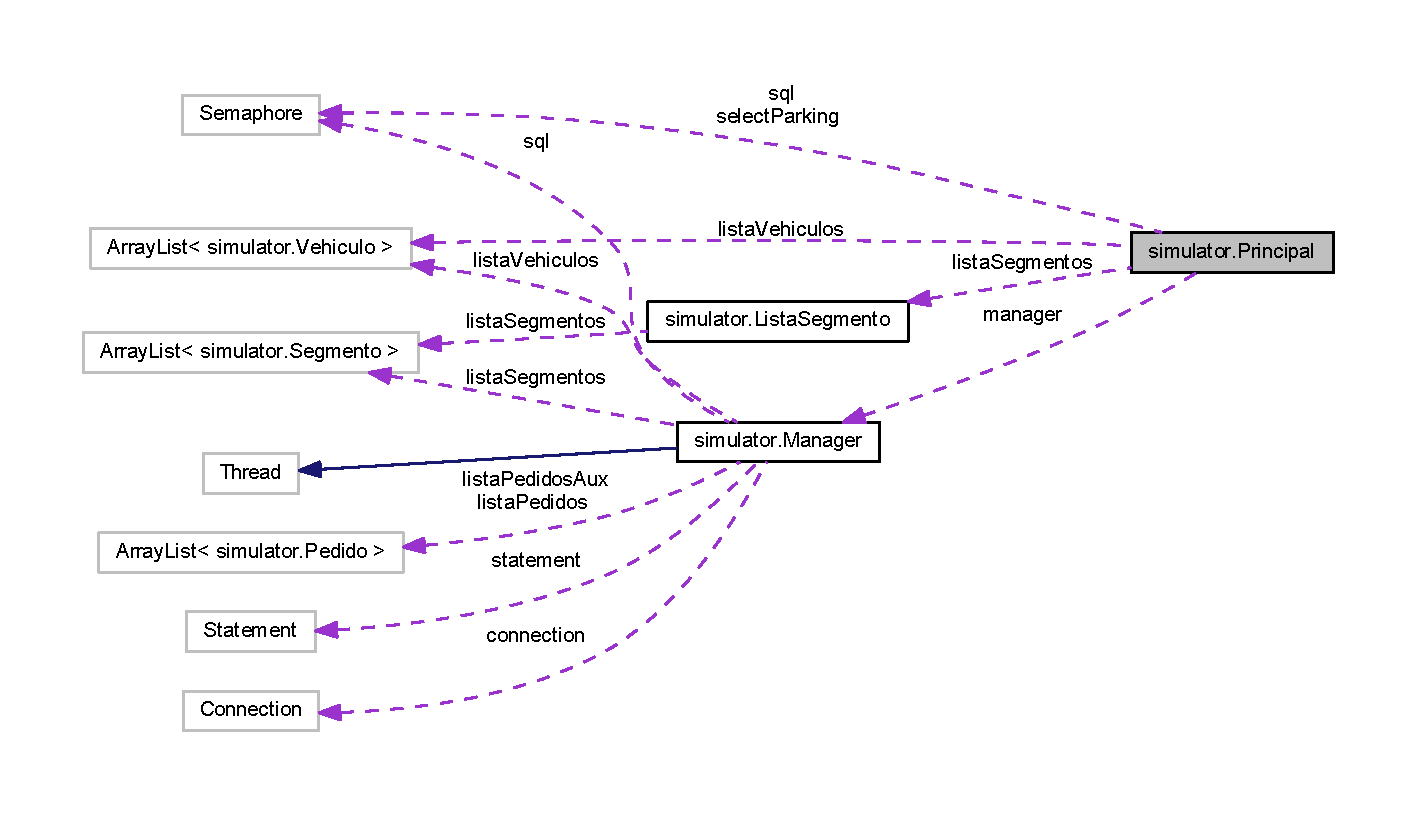
\includegraphics[width=350pt]{classsimulator_1_1_principal__coll__graph}
\end{center}
\end{figure}
\subsection*{Public Member Functions}
\begin{DoxyCompactItemize}
\item 
\mbox{\hyperlink{classsimulator_1_1_principal_afbfaa88badb04d25df7d7c0e36067ef8}{Principal}} ()
\end{DoxyCompactItemize}
\subsection*{Static Public Member Functions}
\begin{DoxyCompactItemize}
\item 
static void \mbox{\hyperlink{classsimulator_1_1_principal_a472c3314a2ab8e7eff9c2539b7818a22}{main}} (String\mbox{[}$\,$\mbox{]} args)
\end{DoxyCompactItemize}


\subsection{Detailed Description}
This is the main class which has the list of vehicles and the list of segments. Both lists objects are initialized in certain points.

\begin{DoxyAuthor}{Author}
Joseba Carnicero, Aitor Eizmendi, Jon Mugica and Marcos Azkarate 
\end{DoxyAuthor}


Definition at line 14 of file Principal.\+java.



\subsection{Constructor \& Destructor Documentation}
\mbox{\Hypertarget{classsimulator_1_1_principal_afbfaa88badb04d25df7d7c0e36067ef8}\label{classsimulator_1_1_principal_afbfaa88badb04d25df7d7c0e36067ef8}} 
\index{simulator\+::\+Principal@{simulator\+::\+Principal}!Principal@{Principal}}
\index{Principal@{Principal}!simulator\+::\+Principal@{simulator\+::\+Principal}}
\subsubsection{\texorpdfstring{Principal()}{Principal()}}
{\footnotesize\ttfamily simulator.\+Principal.\+Principal (\begin{DoxyParamCaption}{ }\end{DoxyParamCaption})}



Definition at line 23 of file Principal.\+java.

Here is the call graph for this function\+:\nopagebreak
\begin{figure}[H]
\begin{center}
\leavevmode
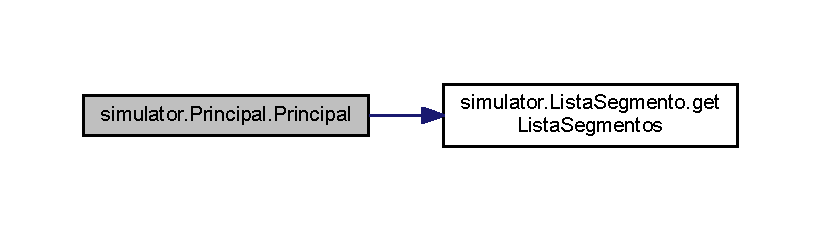
\includegraphics[width=350pt]{classsimulator_1_1_principal_afbfaa88badb04d25df7d7c0e36067ef8_cgraph}
\end{center}
\end{figure}


\subsection{Member Function Documentation}
\mbox{\Hypertarget{classsimulator_1_1_principal_a472c3314a2ab8e7eff9c2539b7818a22}\label{classsimulator_1_1_principal_a472c3314a2ab8e7eff9c2539b7818a22}} 
\index{simulator\+::\+Principal@{simulator\+::\+Principal}!main@{main}}
\index{main@{main}!simulator\+::\+Principal@{simulator\+::\+Principal}}
\subsubsection{\texorpdfstring{main()}{main()}}
{\footnotesize\ttfamily static void simulator.\+Principal.\+main (\begin{DoxyParamCaption}\item[{String \mbox{[}$\,$\mbox{]}}]{args }\end{DoxyParamCaption})\hspace{0.3cm}{\ttfamily [static]}}



Definition at line 57 of file Principal.\+java.

Here is the call graph for this function\+:\nopagebreak
\begin{figure}[H]
\begin{center}
\leavevmode
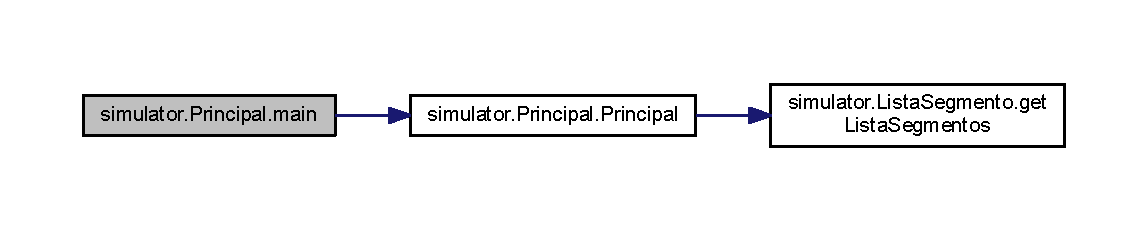
\includegraphics[width=350pt]{classsimulator_1_1_principal_a472c3314a2ab8e7eff9c2539b7818a22_cgraph}
\end{center}
\end{figure}


The documentation for this class was generated from the following file\+:\begin{DoxyCompactItemize}
\item 
java/main/java/simulator/\mbox{\hyperlink{_principal_8java}{Principal.\+java}}\end{DoxyCompactItemize}

\hypertarget{classsimulator_1_1_producto}{}\section{simulator.\+Producto Class Reference}
\label{classsimulator_1_1_producto}\index{simulator.\+Producto@{simulator.\+Producto}}
\subsection*{Public Member Functions}
\begin{DoxyCompactItemize}
\item 
\mbox{\hyperlink{classsimulator_1_1_producto_a8ed98f559ef18c7681a41daf22397ee4}{Producto}} (String nombre, int cantidad, int ws\+ID, int product\+ID)
\item 
String \mbox{\hyperlink{classsimulator_1_1_producto_a1399ce876e1f4cd24c7f1f60da446c1f}{get\+Nombre}} ()
\item 
void \mbox{\hyperlink{classsimulator_1_1_producto_a9db8049ac3a8b1da4117e548bc7b005f}{set\+Nombre}} (String nombre)
\item 
int \mbox{\hyperlink{classsimulator_1_1_producto_af5946c71fa4afa0a7d2040c7aa8e080e}{get\+Cantidad}} ()
\item 
void \mbox{\hyperlink{classsimulator_1_1_producto_ac48ac8d5a9dafc76dde405d60bda6611}{set\+Cantidad}} (int cantidad)
\item 
int \mbox{\hyperlink{classsimulator_1_1_producto_a98f367bc18c4de722ee6a08a4ba0a31e}{get\+Ws\+ID}} ()
\item 
void \mbox{\hyperlink{classsimulator_1_1_producto_af777b058acf8120624ce58d1b5da26d1}{set\+Ws\+ID}} (int ws\+ID)
\item 
int \mbox{\hyperlink{classsimulator_1_1_producto_a28b4edc0f966aa82fc53af57a294e808}{get\+Product\+ID}} ()
\item 
void \mbox{\hyperlink{classsimulator_1_1_producto_aaeb11d43521509b90df6e722e18b9382}{set\+Product\+ID}} (int product\+ID)
\item 
int \mbox{\hyperlink{classsimulator_1_1_producto_a4c2960024b49a7e4d28752ffde30e3c7}{get\+Remaining}} ()
\item 
void \mbox{\hyperlink{classsimulator_1_1_producto_a2df4995ec8370f2af6d72e7d9cd5aa8a}{set\+Remaining}} (int remaining)
\item 
String \mbox{\hyperlink{classsimulator_1_1_producto_a31114900c2dcf40e36fbc4b6b55ce985}{to\+String}} ()
\end{DoxyCompactItemize}


\subsection{Detailed Description}
This is the main class which has the list of vehicles and the list of segments. Both lists objects are initialized in certain points.

\begin{DoxyAuthor}{Author}
Joseba Carnicero, Aitor Eizmendi, Jon Mugica and Marcos Azkarate 
\end{DoxyAuthor}


Definition at line 10 of file Producto.\+java.



\subsection{Constructor \& Destructor Documentation}
\mbox{\Hypertarget{classsimulator_1_1_producto_a8ed98f559ef18c7681a41daf22397ee4}\label{classsimulator_1_1_producto_a8ed98f559ef18c7681a41daf22397ee4}} 
\index{simulator\+::\+Producto@{simulator\+::\+Producto}!Producto@{Producto}}
\index{Producto@{Producto}!simulator\+::\+Producto@{simulator\+::\+Producto}}
\subsubsection{\texorpdfstring{Producto()}{Producto()}}
{\footnotesize\ttfamily simulator.\+Producto.\+Producto (\begin{DoxyParamCaption}\item[{String}]{nombre,  }\item[{int}]{cantidad,  }\item[{int}]{ws\+ID,  }\item[{int}]{product\+ID }\end{DoxyParamCaption})}



Definition at line 17 of file Producto.\+java.



\subsection{Member Function Documentation}
\mbox{\Hypertarget{classsimulator_1_1_producto_af5946c71fa4afa0a7d2040c7aa8e080e}\label{classsimulator_1_1_producto_af5946c71fa4afa0a7d2040c7aa8e080e}} 
\index{simulator\+::\+Producto@{simulator\+::\+Producto}!get\+Cantidad@{get\+Cantidad}}
\index{get\+Cantidad@{get\+Cantidad}!simulator\+::\+Producto@{simulator\+::\+Producto}}
\subsubsection{\texorpdfstring{get\+Cantidad()}{getCantidad()}}
{\footnotesize\ttfamily int simulator.\+Producto.\+get\+Cantidad (\begin{DoxyParamCaption}{ }\end{DoxyParamCaption})}



Definition at line 34 of file Producto.\+java.

\mbox{\Hypertarget{classsimulator_1_1_producto_a1399ce876e1f4cd24c7f1f60da446c1f}\label{classsimulator_1_1_producto_a1399ce876e1f4cd24c7f1f60da446c1f}} 
\index{simulator\+::\+Producto@{simulator\+::\+Producto}!get\+Nombre@{get\+Nombre}}
\index{get\+Nombre@{get\+Nombre}!simulator\+::\+Producto@{simulator\+::\+Producto}}
\subsubsection{\texorpdfstring{get\+Nombre()}{getNombre()}}
{\footnotesize\ttfamily String simulator.\+Producto.\+get\+Nombre (\begin{DoxyParamCaption}{ }\end{DoxyParamCaption})}



Definition at line 26 of file Producto.\+java.

\mbox{\Hypertarget{classsimulator_1_1_producto_a28b4edc0f966aa82fc53af57a294e808}\label{classsimulator_1_1_producto_a28b4edc0f966aa82fc53af57a294e808}} 
\index{simulator\+::\+Producto@{simulator\+::\+Producto}!get\+Product\+ID@{get\+Product\+ID}}
\index{get\+Product\+ID@{get\+Product\+ID}!simulator\+::\+Producto@{simulator\+::\+Producto}}
\subsubsection{\texorpdfstring{get\+Product\+I\+D()}{getProductID()}}
{\footnotesize\ttfamily int simulator.\+Producto.\+get\+Product\+ID (\begin{DoxyParamCaption}{ }\end{DoxyParamCaption})}



Definition at line 50 of file Producto.\+java.

\mbox{\Hypertarget{classsimulator_1_1_producto_a4c2960024b49a7e4d28752ffde30e3c7}\label{classsimulator_1_1_producto_a4c2960024b49a7e4d28752ffde30e3c7}} 
\index{simulator\+::\+Producto@{simulator\+::\+Producto}!get\+Remaining@{get\+Remaining}}
\index{get\+Remaining@{get\+Remaining}!simulator\+::\+Producto@{simulator\+::\+Producto}}
\subsubsection{\texorpdfstring{get\+Remaining()}{getRemaining()}}
{\footnotesize\ttfamily int simulator.\+Producto.\+get\+Remaining (\begin{DoxyParamCaption}{ }\end{DoxyParamCaption})}



Definition at line 58 of file Producto.\+java.

\mbox{\Hypertarget{classsimulator_1_1_producto_a98f367bc18c4de722ee6a08a4ba0a31e}\label{classsimulator_1_1_producto_a98f367bc18c4de722ee6a08a4ba0a31e}} 
\index{simulator\+::\+Producto@{simulator\+::\+Producto}!get\+Ws\+ID@{get\+Ws\+ID}}
\index{get\+Ws\+ID@{get\+Ws\+ID}!simulator\+::\+Producto@{simulator\+::\+Producto}}
\subsubsection{\texorpdfstring{get\+Ws\+I\+D()}{getWsID()}}
{\footnotesize\ttfamily int simulator.\+Producto.\+get\+Ws\+ID (\begin{DoxyParamCaption}{ }\end{DoxyParamCaption})}



Definition at line 42 of file Producto.\+java.

\mbox{\Hypertarget{classsimulator_1_1_producto_ac48ac8d5a9dafc76dde405d60bda6611}\label{classsimulator_1_1_producto_ac48ac8d5a9dafc76dde405d60bda6611}} 
\index{simulator\+::\+Producto@{simulator\+::\+Producto}!set\+Cantidad@{set\+Cantidad}}
\index{set\+Cantidad@{set\+Cantidad}!simulator\+::\+Producto@{simulator\+::\+Producto}}
\subsubsection{\texorpdfstring{set\+Cantidad()}{setCantidad()}}
{\footnotesize\ttfamily void simulator.\+Producto.\+set\+Cantidad (\begin{DoxyParamCaption}\item[{int}]{cantidad }\end{DoxyParamCaption})}



Definition at line 38 of file Producto.\+java.

\mbox{\Hypertarget{classsimulator_1_1_producto_a9db8049ac3a8b1da4117e548bc7b005f}\label{classsimulator_1_1_producto_a9db8049ac3a8b1da4117e548bc7b005f}} 
\index{simulator\+::\+Producto@{simulator\+::\+Producto}!set\+Nombre@{set\+Nombre}}
\index{set\+Nombre@{set\+Nombre}!simulator\+::\+Producto@{simulator\+::\+Producto}}
\subsubsection{\texorpdfstring{set\+Nombre()}{setNombre()}}
{\footnotesize\ttfamily void simulator.\+Producto.\+set\+Nombre (\begin{DoxyParamCaption}\item[{String}]{nombre }\end{DoxyParamCaption})}



Definition at line 30 of file Producto.\+java.

\mbox{\Hypertarget{classsimulator_1_1_producto_aaeb11d43521509b90df6e722e18b9382}\label{classsimulator_1_1_producto_aaeb11d43521509b90df6e722e18b9382}} 
\index{simulator\+::\+Producto@{simulator\+::\+Producto}!set\+Product\+ID@{set\+Product\+ID}}
\index{set\+Product\+ID@{set\+Product\+ID}!simulator\+::\+Producto@{simulator\+::\+Producto}}
\subsubsection{\texorpdfstring{set\+Product\+I\+D()}{setProductID()}}
{\footnotesize\ttfamily void simulator.\+Producto.\+set\+Product\+ID (\begin{DoxyParamCaption}\item[{int}]{product\+ID }\end{DoxyParamCaption})}



Definition at line 54 of file Producto.\+java.

\mbox{\Hypertarget{classsimulator_1_1_producto_a2df4995ec8370f2af6d72e7d9cd5aa8a}\label{classsimulator_1_1_producto_a2df4995ec8370f2af6d72e7d9cd5aa8a}} 
\index{simulator\+::\+Producto@{simulator\+::\+Producto}!set\+Remaining@{set\+Remaining}}
\index{set\+Remaining@{set\+Remaining}!simulator\+::\+Producto@{simulator\+::\+Producto}}
\subsubsection{\texorpdfstring{set\+Remaining()}{setRemaining()}}
{\footnotesize\ttfamily void simulator.\+Producto.\+set\+Remaining (\begin{DoxyParamCaption}\item[{int}]{remaining }\end{DoxyParamCaption})}



Definition at line 62 of file Producto.\+java.

\mbox{\Hypertarget{classsimulator_1_1_producto_af777b058acf8120624ce58d1b5da26d1}\label{classsimulator_1_1_producto_af777b058acf8120624ce58d1b5da26d1}} 
\index{simulator\+::\+Producto@{simulator\+::\+Producto}!set\+Ws\+ID@{set\+Ws\+ID}}
\index{set\+Ws\+ID@{set\+Ws\+ID}!simulator\+::\+Producto@{simulator\+::\+Producto}}
\subsubsection{\texorpdfstring{set\+Ws\+I\+D()}{setWsID()}}
{\footnotesize\ttfamily void simulator.\+Producto.\+set\+Ws\+ID (\begin{DoxyParamCaption}\item[{int}]{ws\+ID }\end{DoxyParamCaption})}



Definition at line 46 of file Producto.\+java.

\mbox{\Hypertarget{classsimulator_1_1_producto_a31114900c2dcf40e36fbc4b6b55ce985}\label{classsimulator_1_1_producto_a31114900c2dcf40e36fbc4b6b55ce985}} 
\index{simulator\+::\+Producto@{simulator\+::\+Producto}!to\+String@{to\+String}}
\index{to\+String@{to\+String}!simulator\+::\+Producto@{simulator\+::\+Producto}}
\subsubsection{\texorpdfstring{to\+String()}{toString()}}
{\footnotesize\ttfamily String simulator.\+Producto.\+to\+String (\begin{DoxyParamCaption}{ }\end{DoxyParamCaption})}



Definition at line 67 of file Producto.\+java.



The documentation for this class was generated from the following file\+:\begin{DoxyCompactItemize}
\item 
java/main/java/simulator/\mbox{\hyperlink{_producto_8java}{Producto.\+java}}\end{DoxyCompactItemize}

\hypertarget{classtest_1_1_producto_test}{}\section{test.\+Producto\+Test Class Reference}
\label{classtest_1_1_producto_test}\index{test.\+Producto\+Test@{test.\+Producto\+Test}}


Collaboration diagram for test.\+Producto\+Test\+:\nopagebreak
\begin{figure}[H]
\begin{center}
\leavevmode
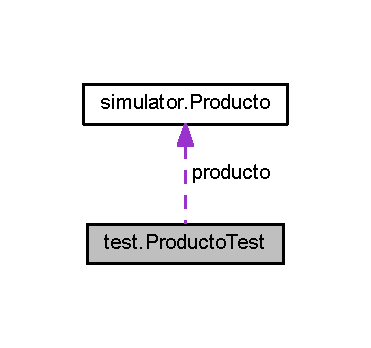
\includegraphics[width=178pt]{classtest_1_1_producto_test__coll__graph}
\end{center}
\end{figure}
\subsection*{Public Member Functions}
\begin{DoxyCompactItemize}
\item 
void \mbox{\hyperlink{classtest_1_1_producto_test_a0ac3e1c91ba64720856242e5aa9fb78b}{before}} ()
\item 
void \mbox{\hyperlink{classtest_1_1_producto_test_ae7f0a17e46f738f4d5bdd4115ffdbff1}{pedido\+Class}} ()
\item 
void \mbox{\hyperlink{classtest_1_1_producto_test_aa7c9f6941160c893d9833c67bf37884b}{pedido\+To\+String}} ()
\end{DoxyCompactItemize}


\subsection{Detailed Description}


Definition at line 11 of file Producto\+Test.\+java.



\subsection{Member Function Documentation}
\mbox{\Hypertarget{classtest_1_1_producto_test_a0ac3e1c91ba64720856242e5aa9fb78b}\label{classtest_1_1_producto_test_a0ac3e1c91ba64720856242e5aa9fb78b}} 
\index{test\+::\+Producto\+Test@{test\+::\+Producto\+Test}!before@{before}}
\index{before@{before}!test\+::\+Producto\+Test@{test\+::\+Producto\+Test}}
\subsubsection{\texorpdfstring{before()}{before()}}
{\footnotesize\ttfamily void test.\+Producto\+Test.\+before (\begin{DoxyParamCaption}{ }\end{DoxyParamCaption})}



Definition at line 16 of file Producto\+Test.\+java.

\mbox{\Hypertarget{classtest_1_1_producto_test_ae7f0a17e46f738f4d5bdd4115ffdbff1}\label{classtest_1_1_producto_test_ae7f0a17e46f738f4d5bdd4115ffdbff1}} 
\index{test\+::\+Producto\+Test@{test\+::\+Producto\+Test}!pedido\+Class@{pedido\+Class}}
\index{pedido\+Class@{pedido\+Class}!test\+::\+Producto\+Test@{test\+::\+Producto\+Test}}
\subsubsection{\texorpdfstring{pedido\+Class()}{pedidoClass()}}
{\footnotesize\ttfamily void test.\+Producto\+Test.\+pedido\+Class (\begin{DoxyParamCaption}{ }\end{DoxyParamCaption})}



Definition at line 21 of file Producto\+Test.\+java.

\mbox{\Hypertarget{classtest_1_1_producto_test_aa7c9f6941160c893d9833c67bf37884b}\label{classtest_1_1_producto_test_aa7c9f6941160c893d9833c67bf37884b}} 
\index{test\+::\+Producto\+Test@{test\+::\+Producto\+Test}!pedido\+To\+String@{pedido\+To\+String}}
\index{pedido\+To\+String@{pedido\+To\+String}!test\+::\+Producto\+Test@{test\+::\+Producto\+Test}}
\subsubsection{\texorpdfstring{pedido\+To\+String()}{pedidoToString()}}
{\footnotesize\ttfamily void test.\+Producto\+Test.\+pedido\+To\+String (\begin{DoxyParamCaption}{ }\end{DoxyParamCaption})}



Definition at line 27 of file Producto\+Test.\+java.

Here is the call graph for this function\+:\nopagebreak
\begin{figure}[H]
\begin{center}
\leavevmode
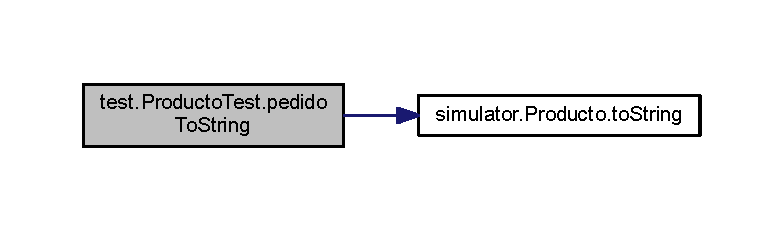
\includegraphics[width=350pt]{classtest_1_1_producto_test_aa7c9f6941160c893d9833c67bf37884b_cgraph}
\end{center}
\end{figure}


The documentation for this class was generated from the following file\+:\begin{DoxyCompactItemize}
\item 
java/test/java/test/\mbox{\hyperlink{_producto_test_8java}{Producto\+Test.\+java}}\end{DoxyCompactItemize}

\hypertarget{classsimulator_1_1_segmento}{}\section{simulator.\+Segmento Class Reference}
\label{classsimulator_1_1_segmento}\index{simulator.\+Segmento@{simulator.\+Segmento}}


Collaboration diagram for simulator.\+Segmento\+:\nopagebreak
\begin{figure}[H]
\begin{center}
\leavevmode
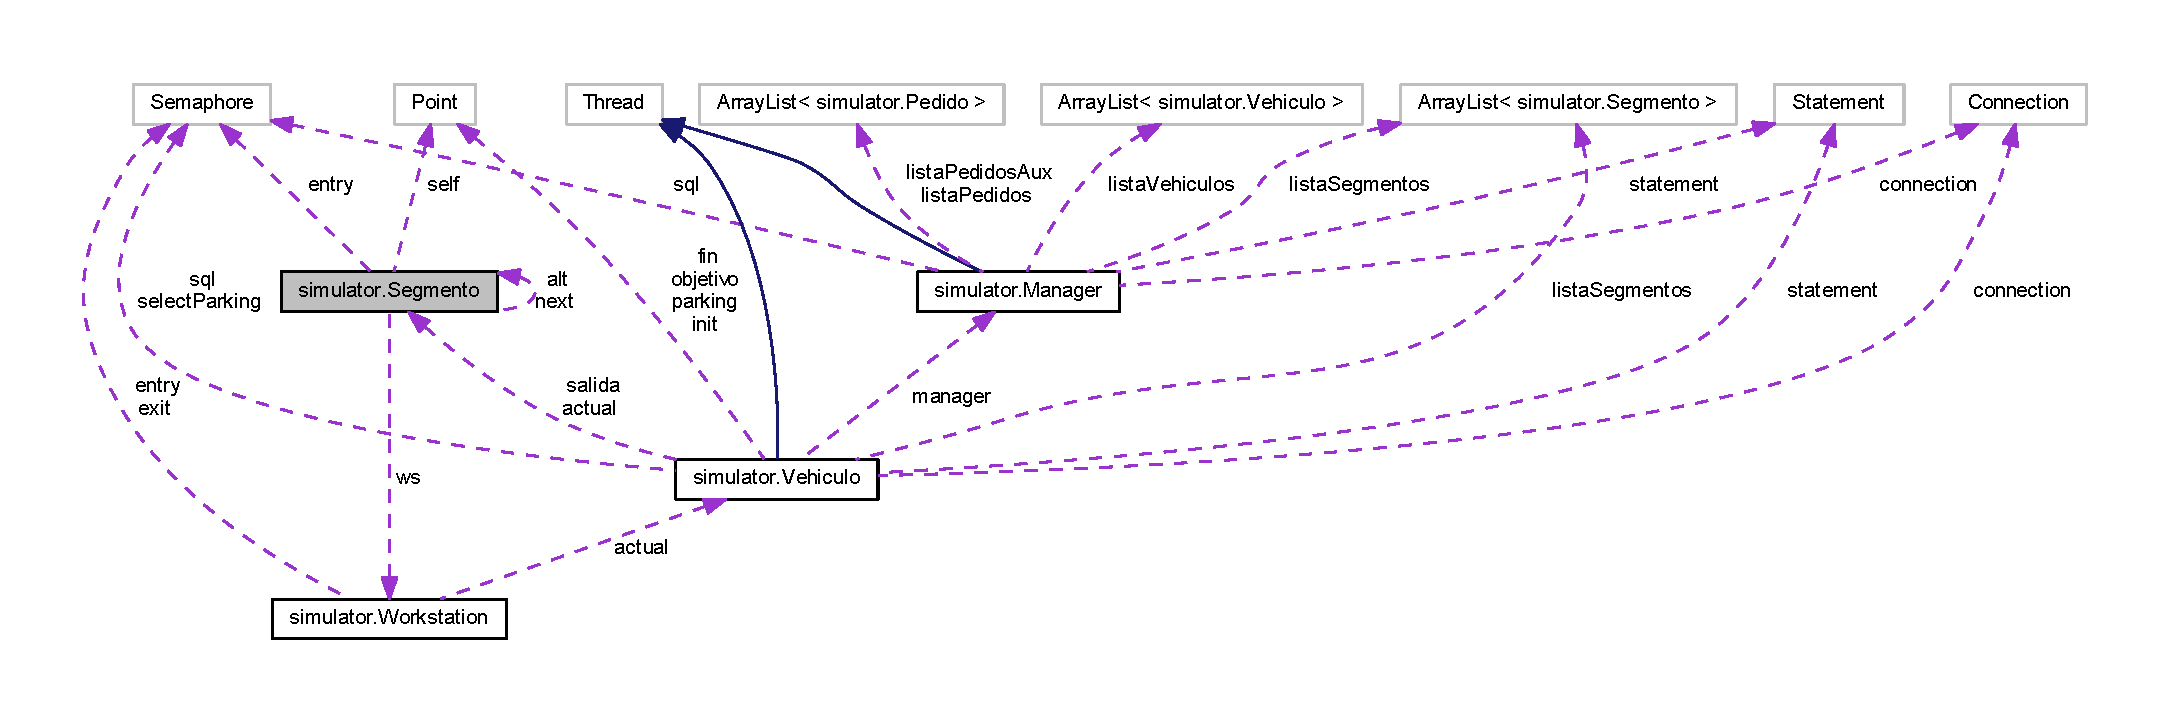
\includegraphics[width=350pt]{classsimulator_1_1_segmento__coll__graph}
\end{center}
\end{figure}
\subsection*{Public Member Functions}
\begin{DoxyCompactItemize}
\item 
\mbox{\hyperlink{classsimulator_1_1_segmento_a441279b72c14ab4e5dab49098eec3dac}{Segmento}} (Point self, \mbox{\hyperlink{classsimulator_1_1_workstation}{Workstation}} ws)
\item 
Point \mbox{\hyperlink{classsimulator_1_1_segmento_a64e246e93f409c3a97798e6b9e63ab42}{get\+Self}} ()
\item 
void \mbox{\hyperlink{classsimulator_1_1_segmento_acc6bd49b531123d4237b514521612840}{set\+Self}} (Point self)
\item 
\mbox{\hyperlink{classsimulator_1_1_segmento}{Segmento}} \mbox{\hyperlink{classsimulator_1_1_segmento_a431ce967de52a69163b325da75c785e2}{get\+Alt}} ()
\item 
void \mbox{\hyperlink{classsimulator_1_1_segmento_a9e0d189b9589c76a15b179de7fe716cb}{set\+Alt}} (\mbox{\hyperlink{classsimulator_1_1_segmento}{Segmento}} \mbox{\hyperlink{classsimulator_1_1_segmento_a0ac22ab701cfb44a6ca41cc831df2695}{alt}})
\item 
\mbox{\hyperlink{classsimulator_1_1_segmento}{Segmento}} \mbox{\hyperlink{classsimulator_1_1_segmento_a1a77a639c0f488b247294f4d57026dc3}{get\+Next}} ()
\item 
void \mbox{\hyperlink{classsimulator_1_1_segmento_a3ff40757a382f8247fd7a3cc70043e58}{set\+Next}} (\mbox{\hyperlink{classsimulator_1_1_segmento}{Segmento}} \mbox{\hyperlink{classsimulator_1_1_segmento_a1cceb01f5ffd65b3a53422fa9e05913c}{next}})
\item 
boolean \mbox{\hyperlink{classsimulator_1_1_segmento_a0da0a40fad9f388e76ce57b6ce072430}{is\+Ocupado}} ()
\item 
void \mbox{\hyperlink{classsimulator_1_1_segmento_a3b8d3958f5ae252c1a9ee2f015040004}{set\+Ocupado}} (boolean ocupado)
\item 
Semaphore \mbox{\hyperlink{classsimulator_1_1_segmento_a023207e6de068a9ebade1b88c477a756}{get\+Entry}} ()
\item 
void \mbox{\hyperlink{classsimulator_1_1_segmento_a412c9085c2cc99e41eb537dd7e0d8e66}{set\+Entry}} (Semaphore entry)
\item 
\mbox{\hyperlink{classsimulator_1_1_workstation}{Workstation}} \mbox{\hyperlink{classsimulator_1_1_segmento_aacd44ec934de39929837f8f3818e2e3b}{get\+Ws}} ()
\item 
void \mbox{\hyperlink{classsimulator_1_1_segmento_a87bee1b2574d78489fb898eff6b45245}{set\+Ws}} (\mbox{\hyperlink{classsimulator_1_1_workstation}{Workstation}} ws)
\end{DoxyCompactItemize}
\subsection*{Public Attributes}
\begin{DoxyCompactItemize}
\item 
\mbox{\hyperlink{classsimulator_1_1_segmento}{Segmento}} \mbox{\hyperlink{classsimulator_1_1_segmento_a0ac22ab701cfb44a6ca41cc831df2695}{alt}}
\item 
\mbox{\hyperlink{classsimulator_1_1_segmento}{Segmento}} \mbox{\hyperlink{classsimulator_1_1_segmento_a1cceb01f5ffd65b3a53422fa9e05913c}{next}}
\end{DoxyCompactItemize}


\subsection{Detailed Description}
This is the Segment class. Segment class contains the actual position, next segment, alt segment, a semaphore and workstation

\begin{DoxyAuthor}{Author}
Joseba Carnicero, Aitor Eizmendi, Jon Mugica and Marcos Azkarate 
\end{DoxyAuthor}


Definition at line 12 of file Segmento.\+java.



\subsection{Constructor \& Destructor Documentation}
\mbox{\Hypertarget{classsimulator_1_1_segmento_a441279b72c14ab4e5dab49098eec3dac}\label{classsimulator_1_1_segmento_a441279b72c14ab4e5dab49098eec3dac}} 
\index{simulator\+::\+Segmento@{simulator\+::\+Segmento}!Segmento@{Segmento}}
\index{Segmento@{Segmento}!simulator\+::\+Segmento@{simulator\+::\+Segmento}}
\subsubsection{\texorpdfstring{Segmento()}{Segmento()}}
{\footnotesize\ttfamily simulator.\+Segmento.\+Segmento (\begin{DoxyParamCaption}\item[{Point}]{self,  }\item[{\mbox{\hyperlink{classsimulator_1_1_workstation}{Workstation}}}]{ws }\end{DoxyParamCaption})}



Definition at line 20 of file Segmento.\+java.



\subsection{Member Function Documentation}
\mbox{\Hypertarget{classsimulator_1_1_segmento_a431ce967de52a69163b325da75c785e2}\label{classsimulator_1_1_segmento_a431ce967de52a69163b325da75c785e2}} 
\index{simulator\+::\+Segmento@{simulator\+::\+Segmento}!get\+Alt@{get\+Alt}}
\index{get\+Alt@{get\+Alt}!simulator\+::\+Segmento@{simulator\+::\+Segmento}}
\subsubsection{\texorpdfstring{get\+Alt()}{getAlt()}}
{\footnotesize\ttfamily \mbox{\hyperlink{classsimulator_1_1_segmento}{Segmento}} simulator.\+Segmento.\+get\+Alt (\begin{DoxyParamCaption}{ }\end{DoxyParamCaption})}



Definition at line 33 of file Segmento.\+java.

\mbox{\Hypertarget{classsimulator_1_1_segmento_a023207e6de068a9ebade1b88c477a756}\label{classsimulator_1_1_segmento_a023207e6de068a9ebade1b88c477a756}} 
\index{simulator\+::\+Segmento@{simulator\+::\+Segmento}!get\+Entry@{get\+Entry}}
\index{get\+Entry@{get\+Entry}!simulator\+::\+Segmento@{simulator\+::\+Segmento}}
\subsubsection{\texorpdfstring{get\+Entry()}{getEntry()}}
{\footnotesize\ttfamily Semaphore simulator.\+Segmento.\+get\+Entry (\begin{DoxyParamCaption}{ }\end{DoxyParamCaption})}



Definition at line 57 of file Segmento.\+java.

\mbox{\Hypertarget{classsimulator_1_1_segmento_a1a77a639c0f488b247294f4d57026dc3}\label{classsimulator_1_1_segmento_a1a77a639c0f488b247294f4d57026dc3}} 
\index{simulator\+::\+Segmento@{simulator\+::\+Segmento}!get\+Next@{get\+Next}}
\index{get\+Next@{get\+Next}!simulator\+::\+Segmento@{simulator\+::\+Segmento}}
\subsubsection{\texorpdfstring{get\+Next()}{getNext()}}
{\footnotesize\ttfamily \mbox{\hyperlink{classsimulator_1_1_segmento}{Segmento}} simulator.\+Segmento.\+get\+Next (\begin{DoxyParamCaption}{ }\end{DoxyParamCaption})}



Definition at line 41 of file Segmento.\+java.

\mbox{\Hypertarget{classsimulator_1_1_segmento_a64e246e93f409c3a97798e6b9e63ab42}\label{classsimulator_1_1_segmento_a64e246e93f409c3a97798e6b9e63ab42}} 
\index{simulator\+::\+Segmento@{simulator\+::\+Segmento}!get\+Self@{get\+Self}}
\index{get\+Self@{get\+Self}!simulator\+::\+Segmento@{simulator\+::\+Segmento}}
\subsubsection{\texorpdfstring{get\+Self()}{getSelf()}}
{\footnotesize\ttfamily Point simulator.\+Segmento.\+get\+Self (\begin{DoxyParamCaption}{ }\end{DoxyParamCaption})}



Definition at line 25 of file Segmento.\+java.

\mbox{\Hypertarget{classsimulator_1_1_segmento_aacd44ec934de39929837f8f3818e2e3b}\label{classsimulator_1_1_segmento_aacd44ec934de39929837f8f3818e2e3b}} 
\index{simulator\+::\+Segmento@{simulator\+::\+Segmento}!get\+Ws@{get\+Ws}}
\index{get\+Ws@{get\+Ws}!simulator\+::\+Segmento@{simulator\+::\+Segmento}}
\subsubsection{\texorpdfstring{get\+Ws()}{getWs()}}
{\footnotesize\ttfamily \mbox{\hyperlink{classsimulator_1_1_workstation}{Workstation}} simulator.\+Segmento.\+get\+Ws (\begin{DoxyParamCaption}{ }\end{DoxyParamCaption})}



Definition at line 65 of file Segmento.\+java.

\mbox{\Hypertarget{classsimulator_1_1_segmento_a0da0a40fad9f388e76ce57b6ce072430}\label{classsimulator_1_1_segmento_a0da0a40fad9f388e76ce57b6ce072430}} 
\index{simulator\+::\+Segmento@{simulator\+::\+Segmento}!is\+Ocupado@{is\+Ocupado}}
\index{is\+Ocupado@{is\+Ocupado}!simulator\+::\+Segmento@{simulator\+::\+Segmento}}
\subsubsection{\texorpdfstring{is\+Ocupado()}{isOcupado()}}
{\footnotesize\ttfamily boolean simulator.\+Segmento.\+is\+Ocupado (\begin{DoxyParamCaption}{ }\end{DoxyParamCaption})}



Definition at line 49 of file Segmento.\+java.

\mbox{\Hypertarget{classsimulator_1_1_segmento_a9e0d189b9589c76a15b179de7fe716cb}\label{classsimulator_1_1_segmento_a9e0d189b9589c76a15b179de7fe716cb}} 
\index{simulator\+::\+Segmento@{simulator\+::\+Segmento}!set\+Alt@{set\+Alt}}
\index{set\+Alt@{set\+Alt}!simulator\+::\+Segmento@{simulator\+::\+Segmento}}
\subsubsection{\texorpdfstring{set\+Alt()}{setAlt()}}
{\footnotesize\ttfamily void simulator.\+Segmento.\+set\+Alt (\begin{DoxyParamCaption}\item[{\mbox{\hyperlink{classsimulator_1_1_segmento}{Segmento}}}]{alt }\end{DoxyParamCaption})}



Definition at line 37 of file Segmento.\+java.

\mbox{\Hypertarget{classsimulator_1_1_segmento_a412c9085c2cc99e41eb537dd7e0d8e66}\label{classsimulator_1_1_segmento_a412c9085c2cc99e41eb537dd7e0d8e66}} 
\index{simulator\+::\+Segmento@{simulator\+::\+Segmento}!set\+Entry@{set\+Entry}}
\index{set\+Entry@{set\+Entry}!simulator\+::\+Segmento@{simulator\+::\+Segmento}}
\subsubsection{\texorpdfstring{set\+Entry()}{setEntry()}}
{\footnotesize\ttfamily void simulator.\+Segmento.\+set\+Entry (\begin{DoxyParamCaption}\item[{Semaphore}]{entry }\end{DoxyParamCaption})}



Definition at line 61 of file Segmento.\+java.

\mbox{\Hypertarget{classsimulator_1_1_segmento_a3ff40757a382f8247fd7a3cc70043e58}\label{classsimulator_1_1_segmento_a3ff40757a382f8247fd7a3cc70043e58}} 
\index{simulator\+::\+Segmento@{simulator\+::\+Segmento}!set\+Next@{set\+Next}}
\index{set\+Next@{set\+Next}!simulator\+::\+Segmento@{simulator\+::\+Segmento}}
\subsubsection{\texorpdfstring{set\+Next()}{setNext()}}
{\footnotesize\ttfamily void simulator.\+Segmento.\+set\+Next (\begin{DoxyParamCaption}\item[{\mbox{\hyperlink{classsimulator_1_1_segmento}{Segmento}}}]{next }\end{DoxyParamCaption})}



Definition at line 45 of file Segmento.\+java.

\mbox{\Hypertarget{classsimulator_1_1_segmento_a3b8d3958f5ae252c1a9ee2f015040004}\label{classsimulator_1_1_segmento_a3b8d3958f5ae252c1a9ee2f015040004}} 
\index{simulator\+::\+Segmento@{simulator\+::\+Segmento}!set\+Ocupado@{set\+Ocupado}}
\index{set\+Ocupado@{set\+Ocupado}!simulator\+::\+Segmento@{simulator\+::\+Segmento}}
\subsubsection{\texorpdfstring{set\+Ocupado()}{setOcupado()}}
{\footnotesize\ttfamily void simulator.\+Segmento.\+set\+Ocupado (\begin{DoxyParamCaption}\item[{boolean}]{ocupado }\end{DoxyParamCaption})}



Definition at line 53 of file Segmento.\+java.

\mbox{\Hypertarget{classsimulator_1_1_segmento_acc6bd49b531123d4237b514521612840}\label{classsimulator_1_1_segmento_acc6bd49b531123d4237b514521612840}} 
\index{simulator\+::\+Segmento@{simulator\+::\+Segmento}!set\+Self@{set\+Self}}
\index{set\+Self@{set\+Self}!simulator\+::\+Segmento@{simulator\+::\+Segmento}}
\subsubsection{\texorpdfstring{set\+Self()}{setSelf()}}
{\footnotesize\ttfamily void simulator.\+Segmento.\+set\+Self (\begin{DoxyParamCaption}\item[{Point}]{self }\end{DoxyParamCaption})}



Definition at line 29 of file Segmento.\+java.

\mbox{\Hypertarget{classsimulator_1_1_segmento_a87bee1b2574d78489fb898eff6b45245}\label{classsimulator_1_1_segmento_a87bee1b2574d78489fb898eff6b45245}} 
\index{simulator\+::\+Segmento@{simulator\+::\+Segmento}!set\+Ws@{set\+Ws}}
\index{set\+Ws@{set\+Ws}!simulator\+::\+Segmento@{simulator\+::\+Segmento}}
\subsubsection{\texorpdfstring{set\+Ws()}{setWs()}}
{\footnotesize\ttfamily void simulator.\+Segmento.\+set\+Ws (\begin{DoxyParamCaption}\item[{\mbox{\hyperlink{classsimulator_1_1_workstation}{Workstation}}}]{ws }\end{DoxyParamCaption})}



Definition at line 69 of file Segmento.\+java.



\subsection{Member Data Documentation}
\mbox{\Hypertarget{classsimulator_1_1_segmento_a0ac22ab701cfb44a6ca41cc831df2695}\label{classsimulator_1_1_segmento_a0ac22ab701cfb44a6ca41cc831df2695}} 
\index{simulator\+::\+Segmento@{simulator\+::\+Segmento}!alt@{alt}}
\index{alt@{alt}!simulator\+::\+Segmento@{simulator\+::\+Segmento}}
\subsubsection{\texorpdfstring{alt}{alt}}
{\footnotesize\ttfamily \mbox{\hyperlink{classsimulator_1_1_segmento}{Segmento}} simulator.\+Segmento.\+alt}



Definition at line 14 of file Segmento.\+java.

\mbox{\Hypertarget{classsimulator_1_1_segmento_a1cceb01f5ffd65b3a53422fa9e05913c}\label{classsimulator_1_1_segmento_a1cceb01f5ffd65b3a53422fa9e05913c}} 
\index{simulator\+::\+Segmento@{simulator\+::\+Segmento}!next@{next}}
\index{next@{next}!simulator\+::\+Segmento@{simulator\+::\+Segmento}}
\subsubsection{\texorpdfstring{next}{next}}
{\footnotesize\ttfamily \mbox{\hyperlink{classsimulator_1_1_segmento}{Segmento}} simulator.\+Segmento.\+next}



Definition at line 15 of file Segmento.\+java.



The documentation for this class was generated from the following file\+:\begin{DoxyCompactItemize}
\item 
java/main/java/simulator/\mbox{\hyperlink{_segmento_8java}{Segmento.\+java}}\end{DoxyCompactItemize}

\hypertarget{classtest_1_1_vehicles_test}{}\section{test.\+Vehicles\+Test Class Reference}
\label{classtest_1_1_vehicles_test}\index{test.\+Vehicles\+Test@{test.\+Vehicles\+Test}}


Inheritance diagram for test.\+Vehicles\+Test\+:\nopagebreak
\begin{figure}[H]
\begin{center}
\leavevmode
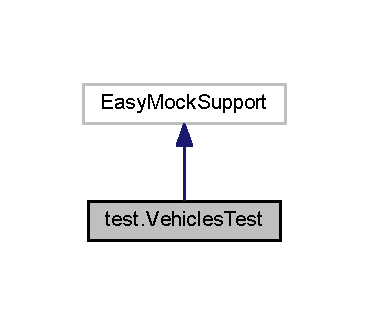
\includegraphics[width=177pt]{classtest_1_1_vehicles_test__inherit__graph}
\end{center}
\end{figure}


Collaboration diagram for test.\+Vehicles\+Test\+:\nopagebreak
\begin{figure}[H]
\begin{center}
\leavevmode
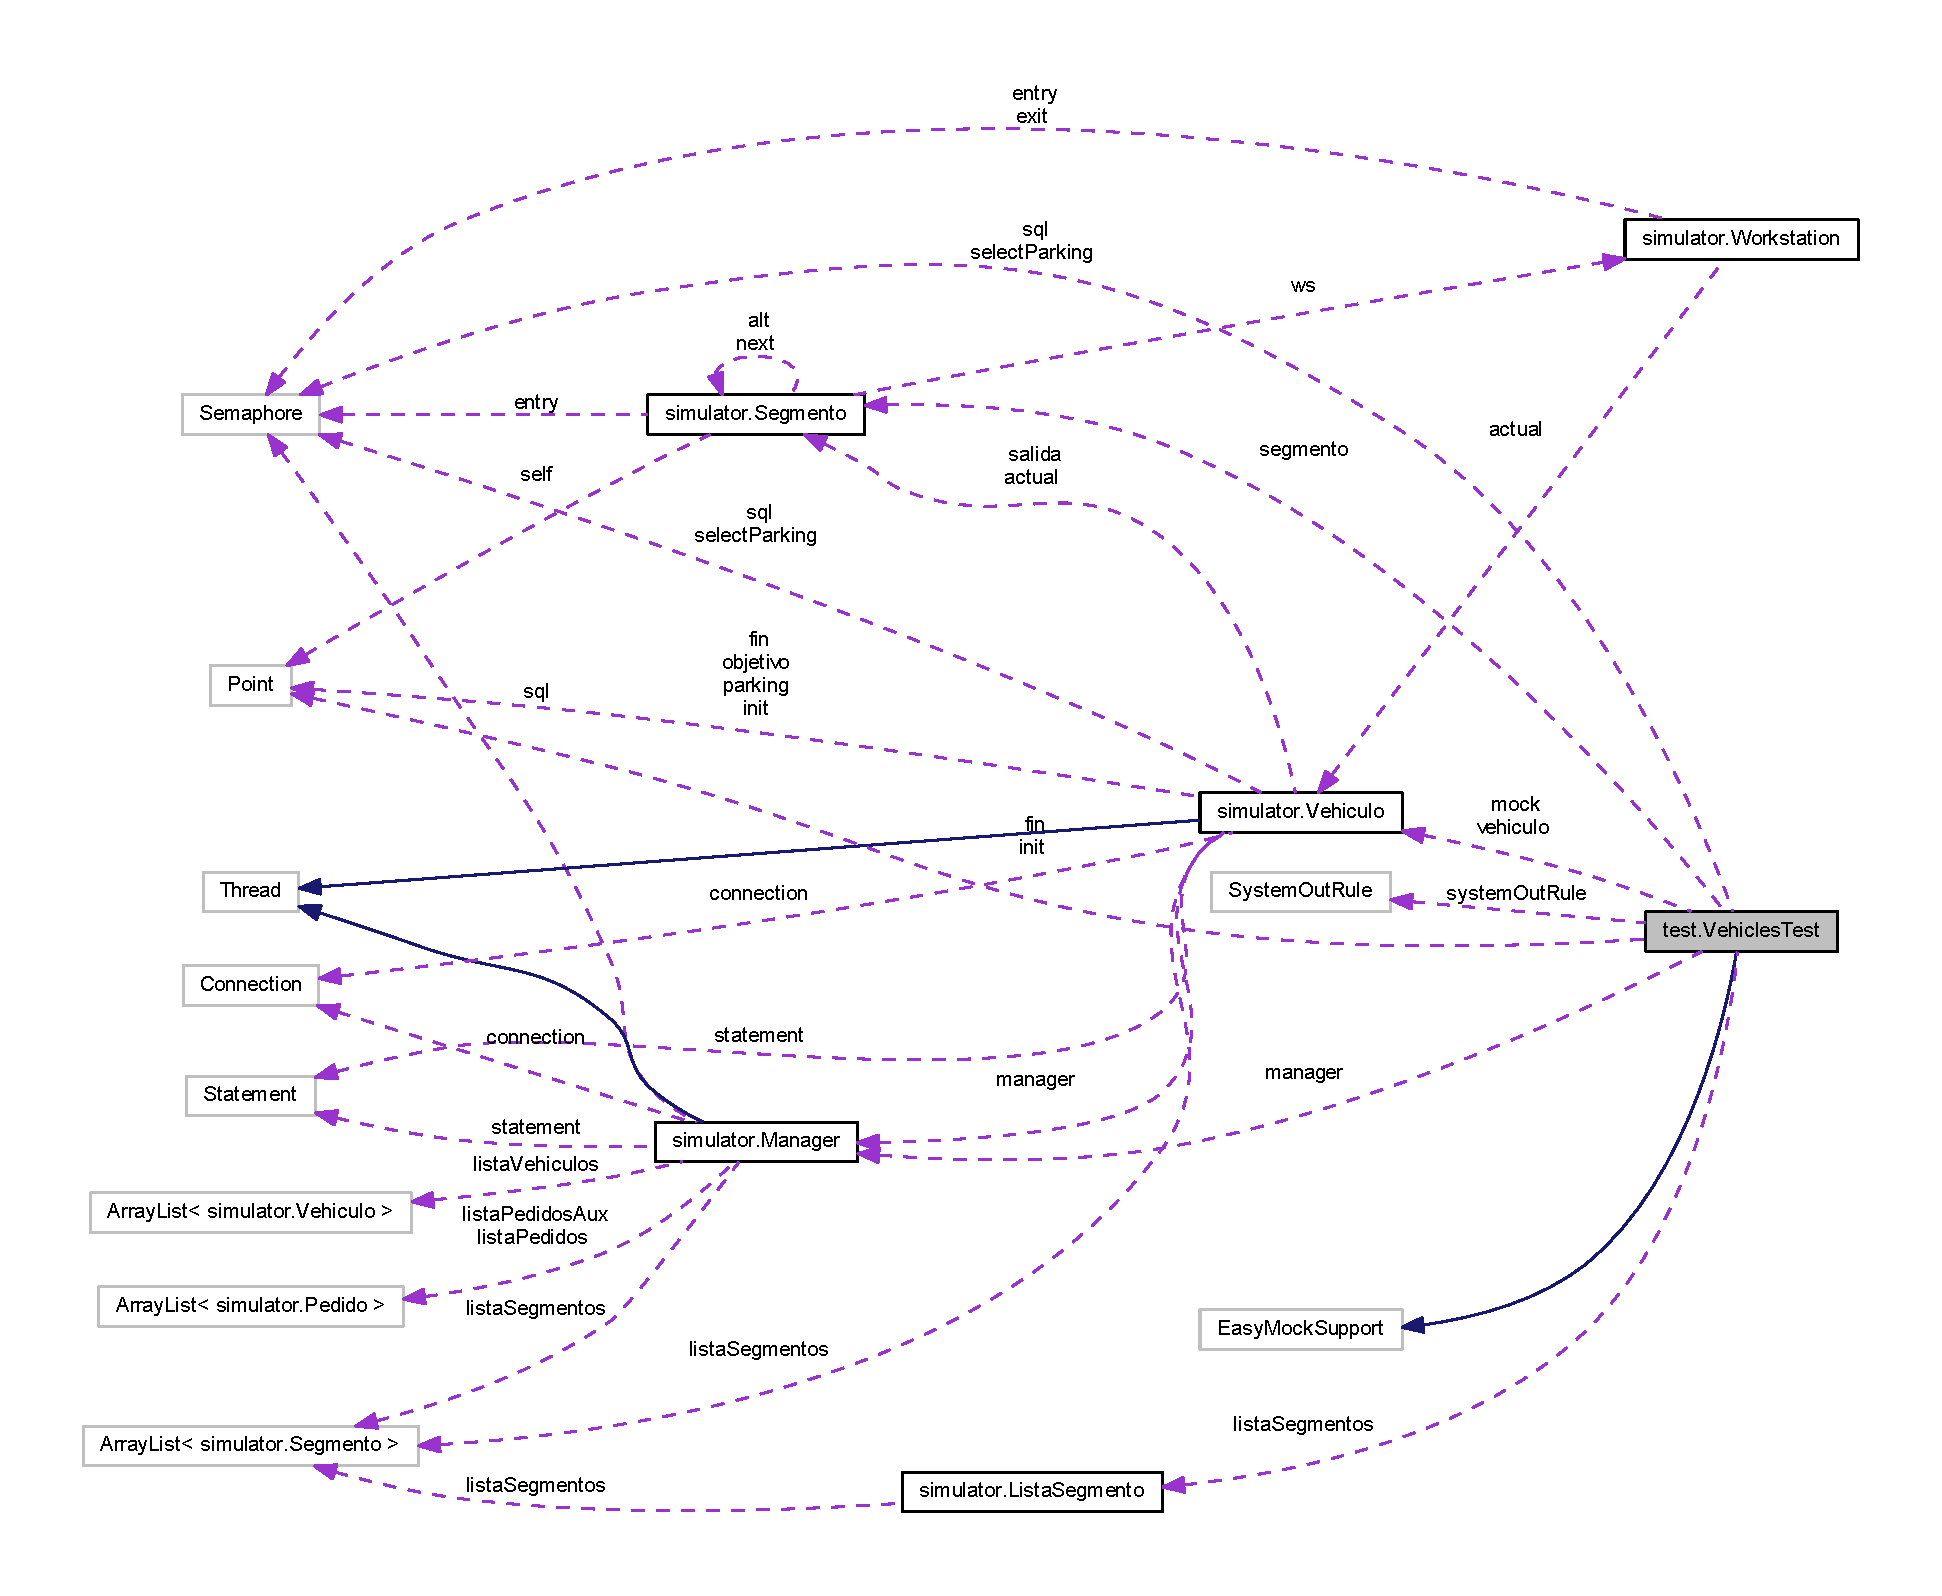
\includegraphics[width=350pt]{classtest_1_1_vehicles_test__coll__graph}
\end{center}
\end{figure}
\subsection*{Public Member Functions}
\begin{DoxyCompactItemize}
\item 
void \mbox{\hyperlink{classtest_1_1_vehicles_test_a1fa47e6164330e08a89695175a6fed1c}{before}} ()
\item 
void \mbox{\hyperlink{classtest_1_1_vehicles_test_a946e0396eb3a4547d8f588408bc82a6d}{buscar\+Actual\+Test}} ()
\item 
void \mbox{\hyperlink{classtest_1_1_vehicles_test_af769f7022f74eff2bbb9a77f5aea83f8}{buscar\+Parking\+True}} ()
\item 
void \mbox{\hyperlink{classtest_1_1_vehicles_test_a7ff46f63103aef8f984b7fbb1f9857fe}{try\+Enter\+Alt\+Test}} ()
\item 
void \mbox{\hyperlink{classtest_1_1_vehicles_test_ac7b3dc490a47ed73391a0a95e8b5445c}{enter\+Next\+Test}} ()
\item 
void \mbox{\hyperlink{classtest_1_1_vehicles_test_ab0a8e244c7fbf7141c528356ce18429a}{enter\+Alt\+Test}} ()
\item 
void \mbox{\hyperlink{classtest_1_1_vehicles_test_a706455718c34d3c7bc6a0cb2917f2ebc}{move\+Test1}} ()
\item 
void \mbox{\hyperlink{classtest_1_1_vehicles_test_a300544e27feeaa4f6dad6d48f45720e9}{move\+Test2}} ()
\item 
void \mbox{\hyperlink{classtest_1_1_vehicles_test_ac6267ff4e71ba311e03c25de20196e65}{move\+Test3}} ()
\item 
void \mbox{\hyperlink{classtest_1_1_vehicles_test_acb2d255019e8718669cb5d6105fd43fa}{move\+Test4}} ()
\item 
void \mbox{\hyperlink{classtest_1_1_vehicles_test_a11f99870b0a4caa2075a2bdeaf910523}{move\+Test5}} ()
\item 
void \mbox{\hyperlink{classtest_1_1_vehicles_test_add2a427b283ac60b944e500f0c66e20b}{move\+Test6}} ()
\item 
void \mbox{\hyperlink{classtest_1_1_vehicles_test_ac0fe870f7fb0e6bd96317b5e8a9c06d0}{move\+Test7}} ()
\item 
void \mbox{\hyperlink{classtest_1_1_vehicles_test_ae80a57f1f29cea08685e8f835d0a6d63}{move\+Test8}} ()
\item 
void \mbox{\hyperlink{classtest_1_1_vehicles_test_ae9e8f3b27af5bb2a0d7b7f52da6ba833}{move\+Test9}} ()
\item 
void \mbox{\hyperlink{classtest_1_1_vehicles_test_a34624265089253eb5d45a7fcffeacd90}{llegada\+Objetivo\+Test}} ()
\item 
void \mbox{\hyperlink{classtest_1_1_vehicles_test_af6b183cd52a3b39d3e565d3e92a85487}{llegada\+Salida\+Test1}} ()
\item 
void \mbox{\hyperlink{classtest_1_1_vehicles_test_a7345ea4de2d3d0f0ebd9fd8d7701c13f}{llegada\+Salida\+Test2}} ()
\item 
void \mbox{\hyperlink{classtest_1_1_vehicles_test_a9b90c693ab518856b021096cefde1e73}{llegada\+Parking}} ()
\end{DoxyCompactItemize}
\subsection*{Public Attributes}
\begin{DoxyCompactItemize}
\item 
final System\+Out\+Rule \mbox{\hyperlink{classtest_1_1_vehicles_test_aaabf0794cb228d330952cb1392a034b0}{system\+Out\+Rule}} = new System\+Out\+Rule().enable\+Log()
\end{DoxyCompactItemize}


\subsection{Detailed Description}


Definition at line 22 of file Vehicles\+Test.\+java.



\subsection{Member Function Documentation}
\mbox{\Hypertarget{classtest_1_1_vehicles_test_a1fa47e6164330e08a89695175a6fed1c}\label{classtest_1_1_vehicles_test_a1fa47e6164330e08a89695175a6fed1c}} 
\index{test\+::\+Vehicles\+Test@{test\+::\+Vehicles\+Test}!before@{before}}
\index{before@{before}!test\+::\+Vehicles\+Test@{test\+::\+Vehicles\+Test}}
\subsubsection{\texorpdfstring{before()}{before()}}
{\footnotesize\ttfamily void test.\+Vehicles\+Test.\+before (\begin{DoxyParamCaption}{ }\end{DoxyParamCaption})}



Definition at line 36 of file Vehicles\+Test.\+java.

Here is the call graph for this function\+:\nopagebreak
\begin{figure}[H]
\begin{center}
\leavevmode
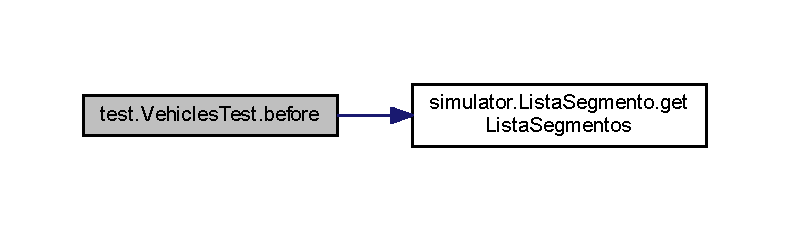
\includegraphics[width=350pt]{classtest_1_1_vehicles_test_a1fa47e6164330e08a89695175a6fed1c_cgraph}
\end{center}
\end{figure}
\mbox{\Hypertarget{classtest_1_1_vehicles_test_a946e0396eb3a4547d8f588408bc82a6d}\label{classtest_1_1_vehicles_test_a946e0396eb3a4547d8f588408bc82a6d}} 
\index{test\+::\+Vehicles\+Test@{test\+::\+Vehicles\+Test}!buscar\+Actual\+Test@{buscar\+Actual\+Test}}
\index{buscar\+Actual\+Test@{buscar\+Actual\+Test}!test\+::\+Vehicles\+Test@{test\+::\+Vehicles\+Test}}
\subsubsection{\texorpdfstring{buscar\+Actual\+Test()}{buscarActualTest()}}
{\footnotesize\ttfamily void test.\+Vehicles\+Test.\+buscar\+Actual\+Test (\begin{DoxyParamCaption}{ }\end{DoxyParamCaption})}



Definition at line 65 of file Vehicles\+Test.\+java.

Here is the call graph for this function\+:\nopagebreak
\begin{figure}[H]
\begin{center}
\leavevmode
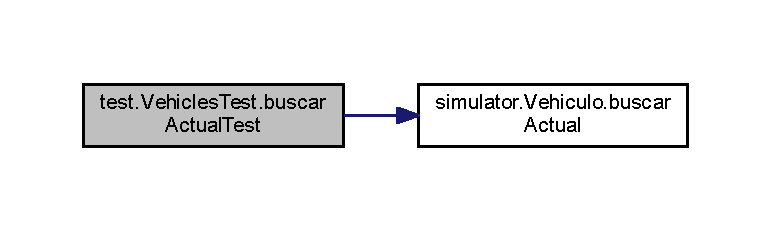
\includegraphics[width=350pt]{classtest_1_1_vehicles_test_a946e0396eb3a4547d8f588408bc82a6d_cgraph}
\end{center}
\end{figure}
\mbox{\Hypertarget{classtest_1_1_vehicles_test_af769f7022f74eff2bbb9a77f5aea83f8}\label{classtest_1_1_vehicles_test_af769f7022f74eff2bbb9a77f5aea83f8}} 
\index{test\+::\+Vehicles\+Test@{test\+::\+Vehicles\+Test}!buscar\+Parking\+True@{buscar\+Parking\+True}}
\index{buscar\+Parking\+True@{buscar\+Parking\+True}!test\+::\+Vehicles\+Test@{test\+::\+Vehicles\+Test}}
\subsubsection{\texorpdfstring{buscar\+Parking\+True()}{buscarParkingTrue()}}
{\footnotesize\ttfamily void test.\+Vehicles\+Test.\+buscar\+Parking\+True (\begin{DoxyParamCaption}{ }\end{DoxyParamCaption})}



Definition at line 75 of file Vehicles\+Test.\+java.

Here is the call graph for this function\+:\nopagebreak
\begin{figure}[H]
\begin{center}
\leavevmode
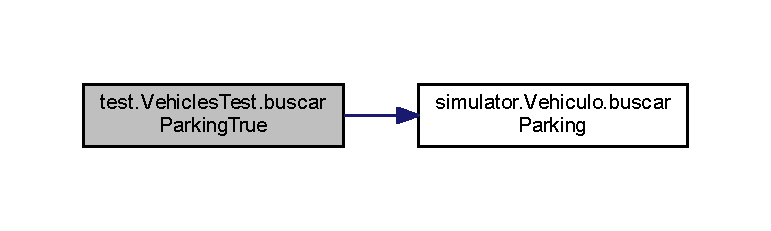
\includegraphics[width=350pt]{classtest_1_1_vehicles_test_af769f7022f74eff2bbb9a77f5aea83f8_cgraph}
\end{center}
\end{figure}
\mbox{\Hypertarget{classtest_1_1_vehicles_test_ab0a8e244c7fbf7141c528356ce18429a}\label{classtest_1_1_vehicles_test_ab0a8e244c7fbf7141c528356ce18429a}} 
\index{test\+::\+Vehicles\+Test@{test\+::\+Vehicles\+Test}!enter\+Alt\+Test@{enter\+Alt\+Test}}
\index{enter\+Alt\+Test@{enter\+Alt\+Test}!test\+::\+Vehicles\+Test@{test\+::\+Vehicles\+Test}}
\subsubsection{\texorpdfstring{enter\+Alt\+Test()}{enterAltTest()}}
{\footnotesize\ttfamily void test.\+Vehicles\+Test.\+enter\+Alt\+Test (\begin{DoxyParamCaption}{ }\end{DoxyParamCaption})}



Definition at line 111 of file Vehicles\+Test.\+java.

Here is the call graph for this function\+:\nopagebreak
\begin{figure}[H]
\begin{center}
\leavevmode
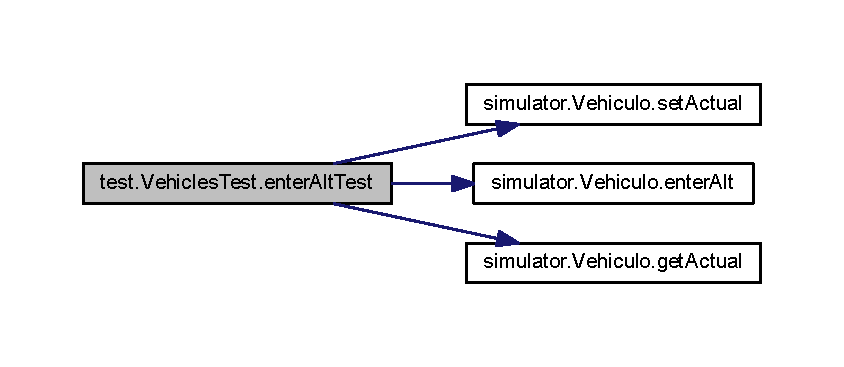
\includegraphics[width=350pt]{classtest_1_1_vehicles_test_ab0a8e244c7fbf7141c528356ce18429a_cgraph}
\end{center}
\end{figure}
\mbox{\Hypertarget{classtest_1_1_vehicles_test_ac7b3dc490a47ed73391a0a95e8b5445c}\label{classtest_1_1_vehicles_test_ac7b3dc490a47ed73391a0a95e8b5445c}} 
\index{test\+::\+Vehicles\+Test@{test\+::\+Vehicles\+Test}!enter\+Next\+Test@{enter\+Next\+Test}}
\index{enter\+Next\+Test@{enter\+Next\+Test}!test\+::\+Vehicles\+Test@{test\+::\+Vehicles\+Test}}
\subsubsection{\texorpdfstring{enter\+Next\+Test()}{enterNextTest()}}
{\footnotesize\ttfamily void test.\+Vehicles\+Test.\+enter\+Next\+Test (\begin{DoxyParamCaption}{ }\end{DoxyParamCaption})}



Definition at line 99 of file Vehicles\+Test.\+java.

Here is the call graph for this function\+:\nopagebreak
\begin{figure}[H]
\begin{center}
\leavevmode
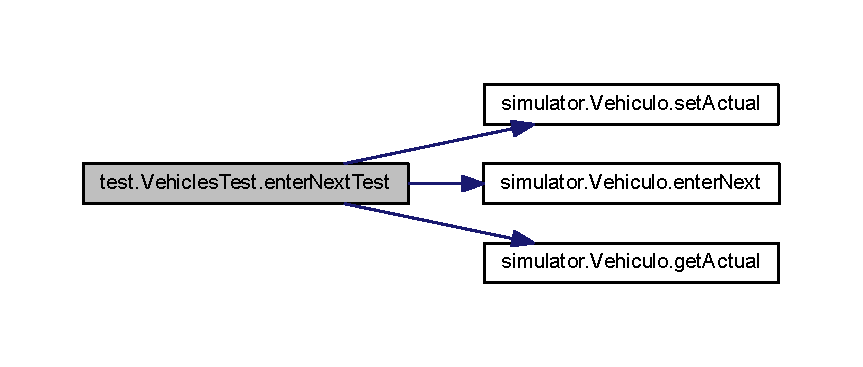
\includegraphics[width=350pt]{classtest_1_1_vehicles_test_ac7b3dc490a47ed73391a0a95e8b5445c_cgraph}
\end{center}
\end{figure}
\mbox{\Hypertarget{classtest_1_1_vehicles_test_a34624265089253eb5d45a7fcffeacd90}\label{classtest_1_1_vehicles_test_a34624265089253eb5d45a7fcffeacd90}} 
\index{test\+::\+Vehicles\+Test@{test\+::\+Vehicles\+Test}!llegada\+Objetivo\+Test@{llegada\+Objetivo\+Test}}
\index{llegada\+Objetivo\+Test@{llegada\+Objetivo\+Test}!test\+::\+Vehicles\+Test@{test\+::\+Vehicles\+Test}}
\subsubsection{\texorpdfstring{llegada\+Objetivo\+Test()}{llegadaObjetivoTest()}}
{\footnotesize\ttfamily void test.\+Vehicles\+Test.\+llegada\+Objetivo\+Test (\begin{DoxyParamCaption}{ }\end{DoxyParamCaption})}



Definition at line 226 of file Vehicles\+Test.\+java.

Here is the call graph for this function\+:\nopagebreak
\begin{figure}[H]
\begin{center}
\leavevmode
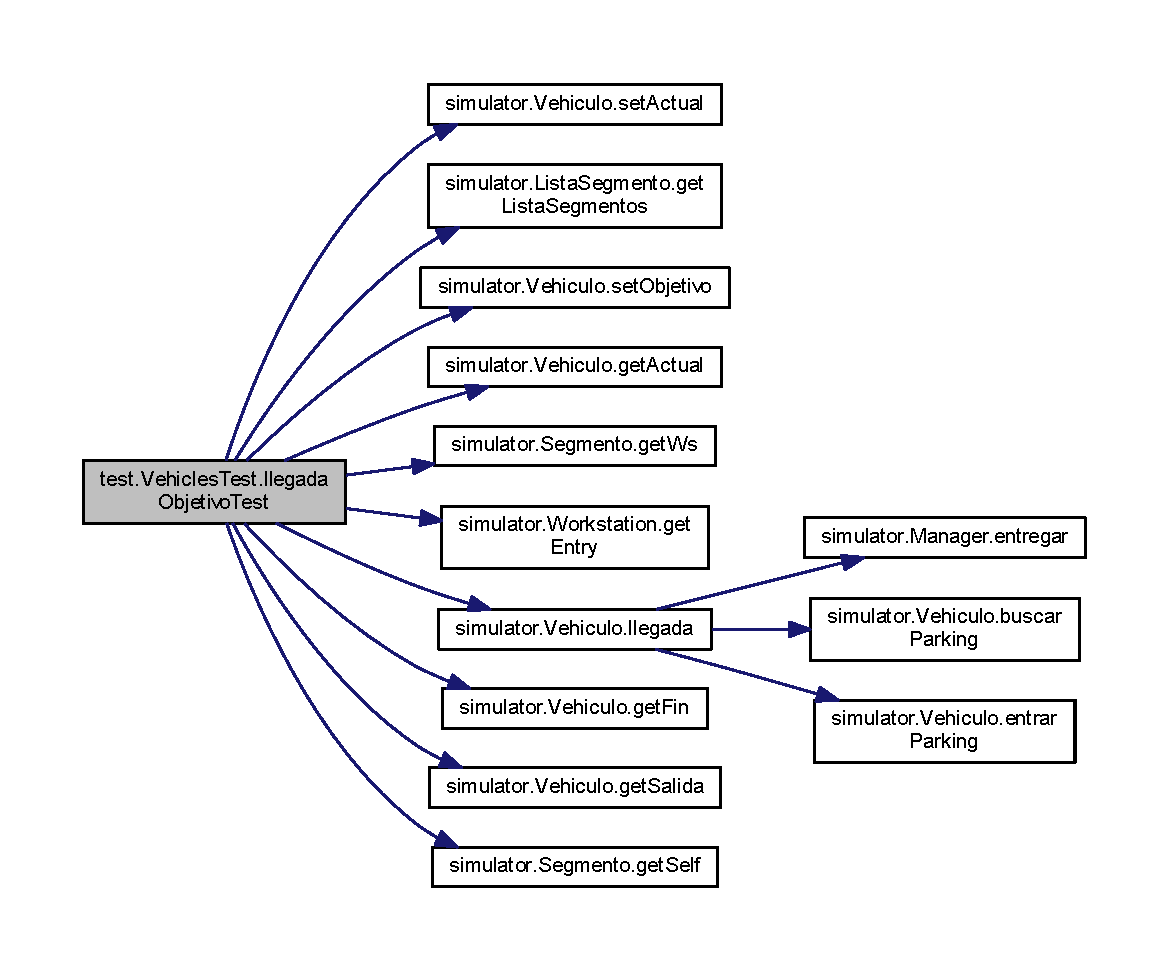
\includegraphics[width=350pt]{classtest_1_1_vehicles_test_a34624265089253eb5d45a7fcffeacd90_cgraph}
\end{center}
\end{figure}
\mbox{\Hypertarget{classtest_1_1_vehicles_test_a9b90c693ab518856b021096cefde1e73}\label{classtest_1_1_vehicles_test_a9b90c693ab518856b021096cefde1e73}} 
\index{test\+::\+Vehicles\+Test@{test\+::\+Vehicles\+Test}!llegada\+Parking@{llegada\+Parking}}
\index{llegada\+Parking@{llegada\+Parking}!test\+::\+Vehicles\+Test@{test\+::\+Vehicles\+Test}}
\subsubsection{\texorpdfstring{llegada\+Parking()}{llegadaParking()}}
{\footnotesize\ttfamily void test.\+Vehicles\+Test.\+llegada\+Parking (\begin{DoxyParamCaption}{ }\end{DoxyParamCaption})}



Definition at line 265 of file Vehicles\+Test.\+java.

Here is the call graph for this function\+:\nopagebreak
\begin{figure}[H]
\begin{center}
\leavevmode
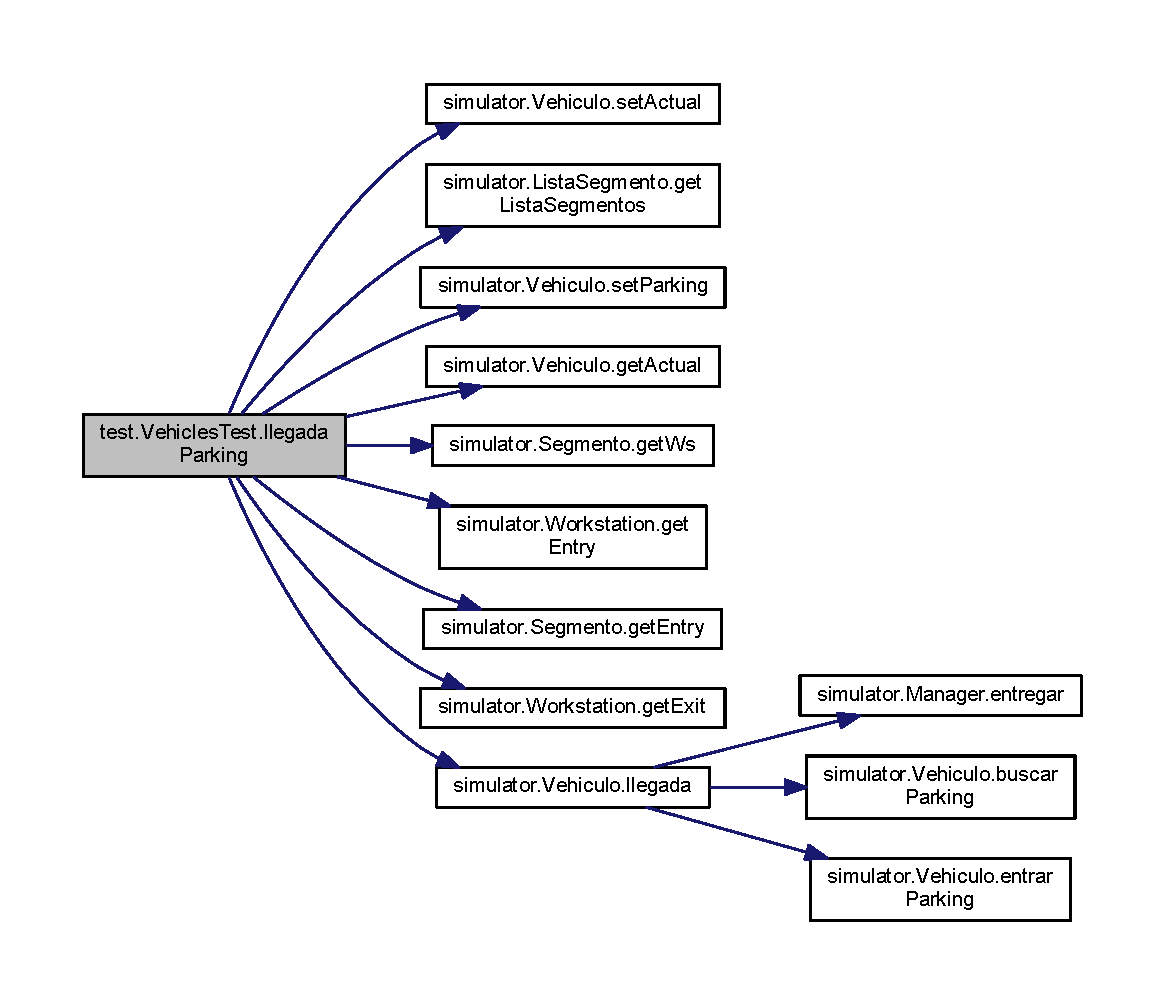
\includegraphics[width=350pt]{classtest_1_1_vehicles_test_a9b90c693ab518856b021096cefde1e73_cgraph}
\end{center}
\end{figure}
\mbox{\Hypertarget{classtest_1_1_vehicles_test_af6b183cd52a3b39d3e565d3e92a85487}\label{classtest_1_1_vehicles_test_af6b183cd52a3b39d3e565d3e92a85487}} 
\index{test\+::\+Vehicles\+Test@{test\+::\+Vehicles\+Test}!llegada\+Salida\+Test1@{llegada\+Salida\+Test1}}
\index{llegada\+Salida\+Test1@{llegada\+Salida\+Test1}!test\+::\+Vehicles\+Test@{test\+::\+Vehicles\+Test}}
\subsubsection{\texorpdfstring{llegada\+Salida\+Test1()}{llegadaSalidaTest1()}}
{\footnotesize\ttfamily void test.\+Vehicles\+Test.\+llegada\+Salida\+Test1 (\begin{DoxyParamCaption}{ }\end{DoxyParamCaption})}



Definition at line 235 of file Vehicles\+Test.\+java.

Here is the call graph for this function\+:\nopagebreak
\begin{figure}[H]
\begin{center}
\leavevmode
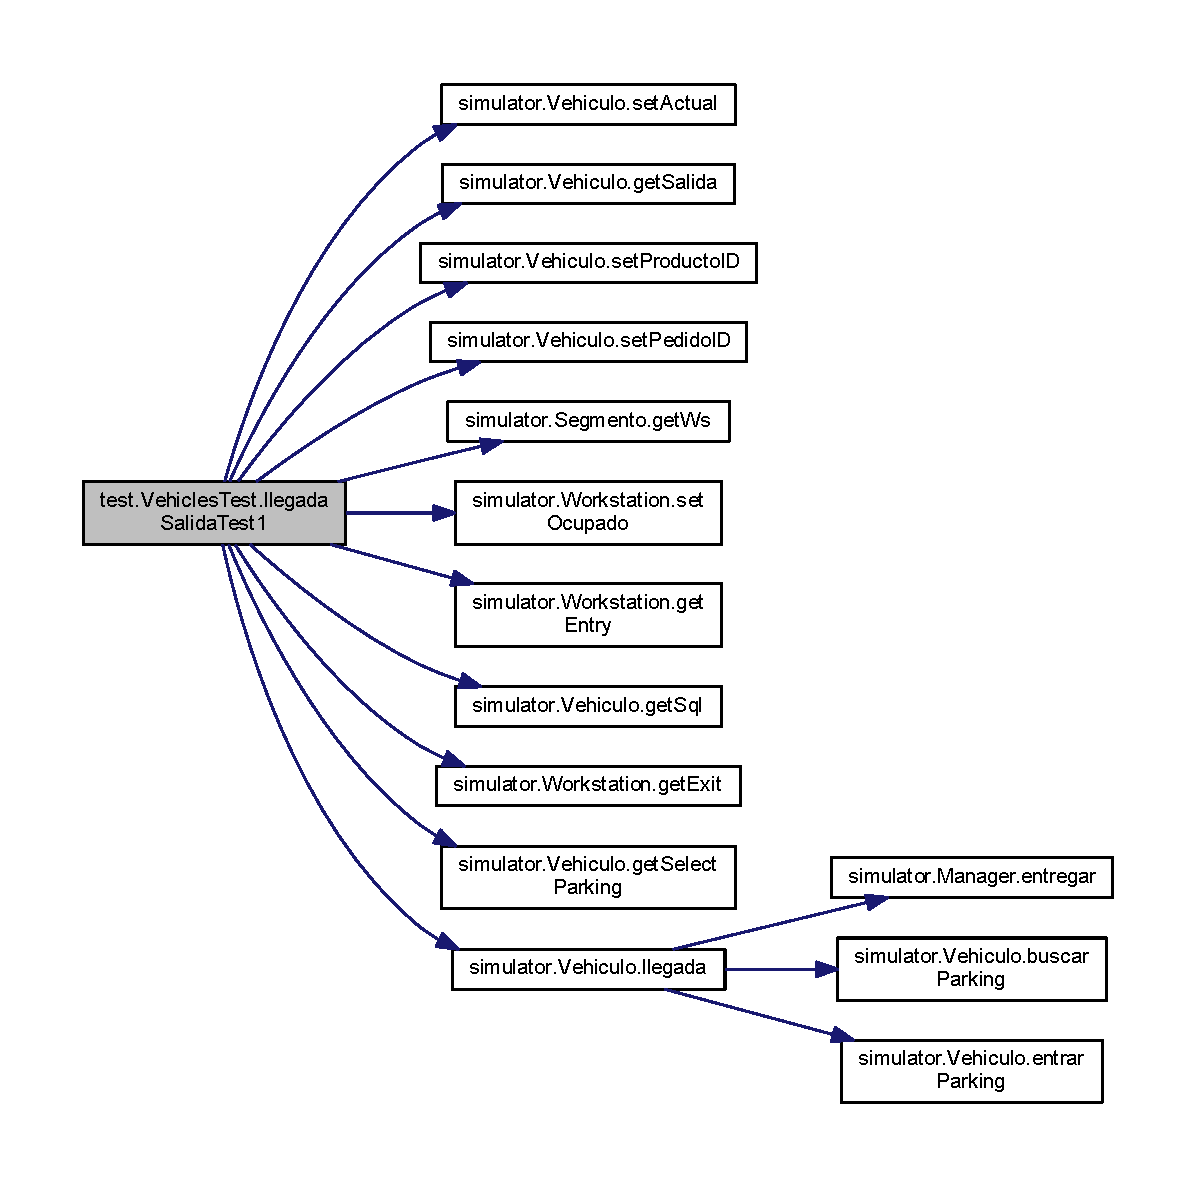
\includegraphics[width=350pt]{classtest_1_1_vehicles_test_af6b183cd52a3b39d3e565d3e92a85487_cgraph}
\end{center}
\end{figure}
\mbox{\Hypertarget{classtest_1_1_vehicles_test_a7345ea4de2d3d0f0ebd9fd8d7701c13f}\label{classtest_1_1_vehicles_test_a7345ea4de2d3d0f0ebd9fd8d7701c13f}} 
\index{test\+::\+Vehicles\+Test@{test\+::\+Vehicles\+Test}!llegada\+Salida\+Test2@{llegada\+Salida\+Test2}}
\index{llegada\+Salida\+Test2@{llegada\+Salida\+Test2}!test\+::\+Vehicles\+Test@{test\+::\+Vehicles\+Test}}
\subsubsection{\texorpdfstring{llegada\+Salida\+Test2()}{llegadaSalidaTest2()}}
{\footnotesize\ttfamily void test.\+Vehicles\+Test.\+llegada\+Salida\+Test2 (\begin{DoxyParamCaption}{ }\end{DoxyParamCaption})}



Definition at line 249 of file Vehicles\+Test.\+java.

Here is the call graph for this function\+:\nopagebreak
\begin{figure}[H]
\begin{center}
\leavevmode
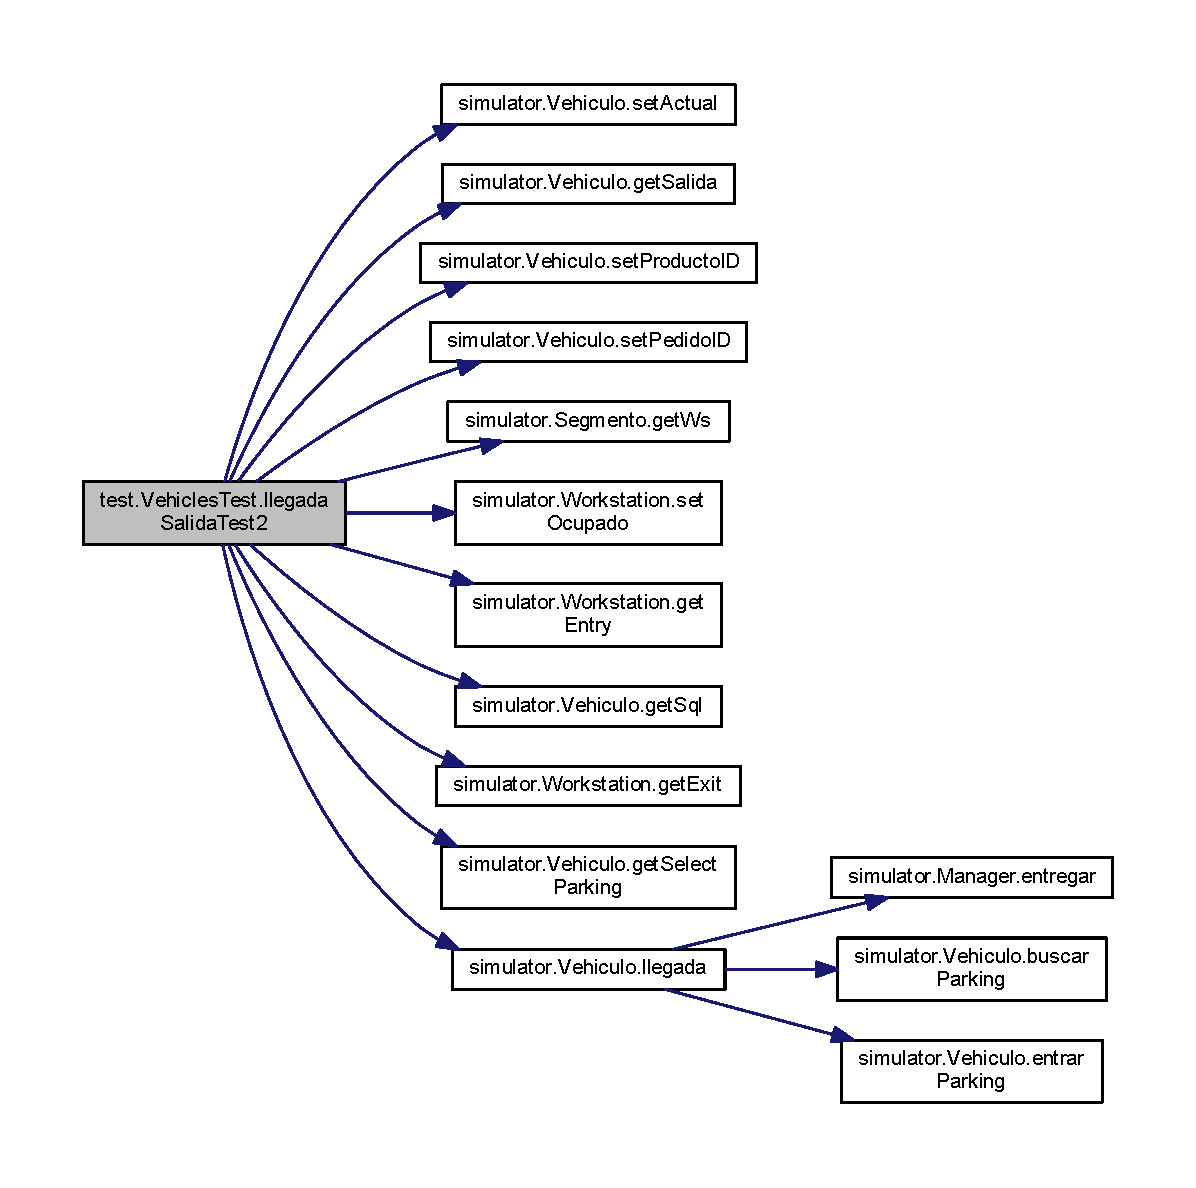
\includegraphics[width=350pt]{classtest_1_1_vehicles_test_a7345ea4de2d3d0f0ebd9fd8d7701c13f_cgraph}
\end{center}
\end{figure}
\mbox{\Hypertarget{classtest_1_1_vehicles_test_a706455718c34d3c7bc6a0cb2917f2ebc}\label{classtest_1_1_vehicles_test_a706455718c34d3c7bc6a0cb2917f2ebc}} 
\index{test\+::\+Vehicles\+Test@{test\+::\+Vehicles\+Test}!move\+Test1@{move\+Test1}}
\index{move\+Test1@{move\+Test1}!test\+::\+Vehicles\+Test@{test\+::\+Vehicles\+Test}}
\subsubsection{\texorpdfstring{move\+Test1()}{moveTest1()}}
{\footnotesize\ttfamily void test.\+Vehicles\+Test.\+move\+Test1 (\begin{DoxyParamCaption}{ }\end{DoxyParamCaption})}



Definition at line 122 of file Vehicles\+Test.\+java.

Here is the call graph for this function\+:\nopagebreak
\begin{figure}[H]
\begin{center}
\leavevmode
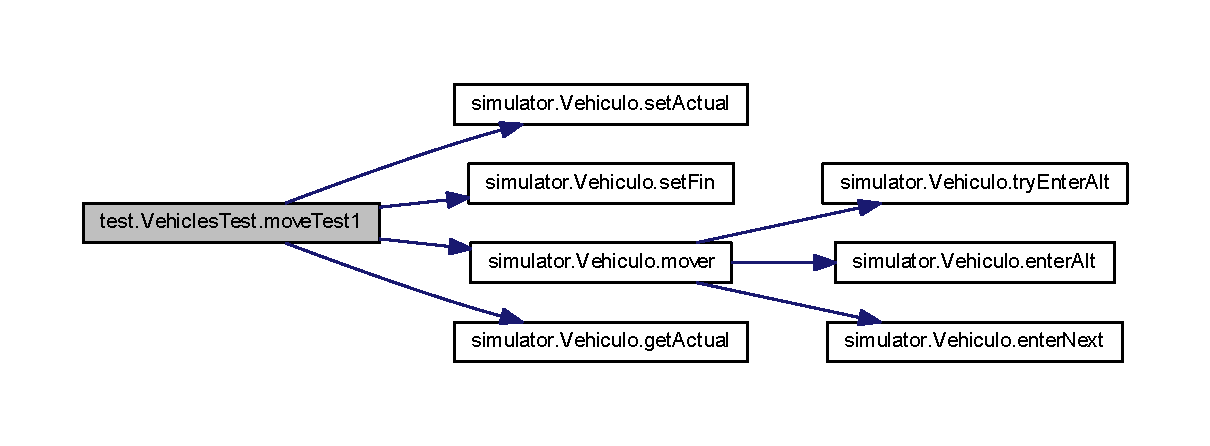
\includegraphics[width=350pt]{classtest_1_1_vehicles_test_a706455718c34d3c7bc6a0cb2917f2ebc_cgraph}
\end{center}
\end{figure}
\mbox{\Hypertarget{classtest_1_1_vehicles_test_a300544e27feeaa4f6dad6d48f45720e9}\label{classtest_1_1_vehicles_test_a300544e27feeaa4f6dad6d48f45720e9}} 
\index{test\+::\+Vehicles\+Test@{test\+::\+Vehicles\+Test}!move\+Test2@{move\+Test2}}
\index{move\+Test2@{move\+Test2}!test\+::\+Vehicles\+Test@{test\+::\+Vehicles\+Test}}
\subsubsection{\texorpdfstring{move\+Test2()}{moveTest2()}}
{\footnotesize\ttfamily void test.\+Vehicles\+Test.\+move\+Test2 (\begin{DoxyParamCaption}{ }\end{DoxyParamCaption})}



Definition at line 132 of file Vehicles\+Test.\+java.

Here is the call graph for this function\+:\nopagebreak
\begin{figure}[H]
\begin{center}
\leavevmode
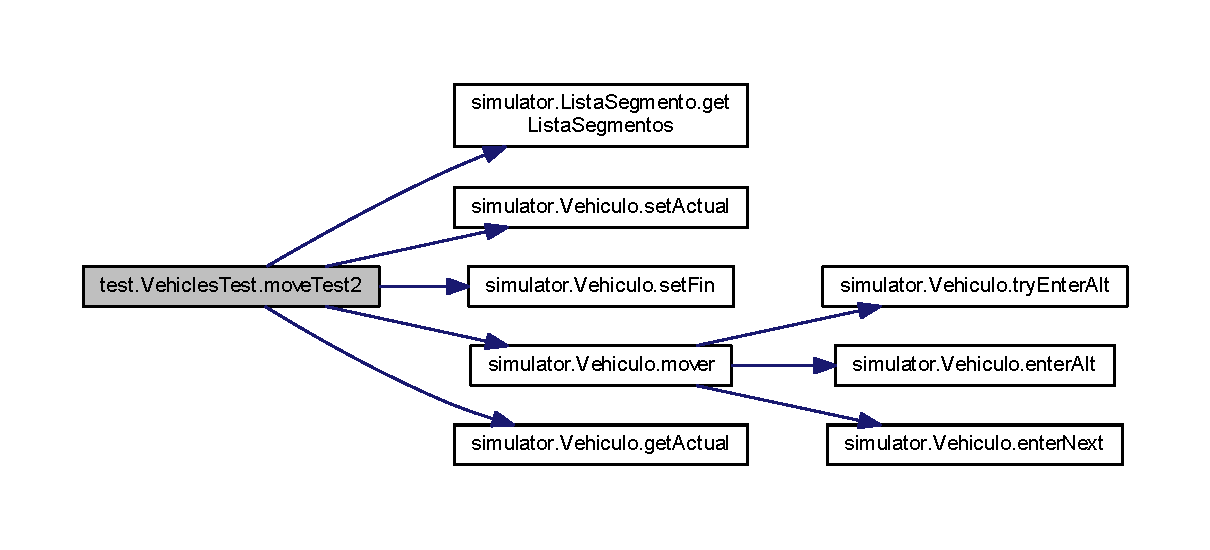
\includegraphics[width=350pt]{classtest_1_1_vehicles_test_a300544e27feeaa4f6dad6d48f45720e9_cgraph}
\end{center}
\end{figure}
\mbox{\Hypertarget{classtest_1_1_vehicles_test_ac6267ff4e71ba311e03c25de20196e65}\label{classtest_1_1_vehicles_test_ac6267ff4e71ba311e03c25de20196e65}} 
\index{test\+::\+Vehicles\+Test@{test\+::\+Vehicles\+Test}!move\+Test3@{move\+Test3}}
\index{move\+Test3@{move\+Test3}!test\+::\+Vehicles\+Test@{test\+::\+Vehicles\+Test}}
\subsubsection{\texorpdfstring{move\+Test3()}{moveTest3()}}
{\footnotesize\ttfamily void test.\+Vehicles\+Test.\+move\+Test3 (\begin{DoxyParamCaption}{ }\end{DoxyParamCaption})}



Definition at line 143 of file Vehicles\+Test.\+java.

Here is the call graph for this function\+:\nopagebreak
\begin{figure}[H]
\begin{center}
\leavevmode
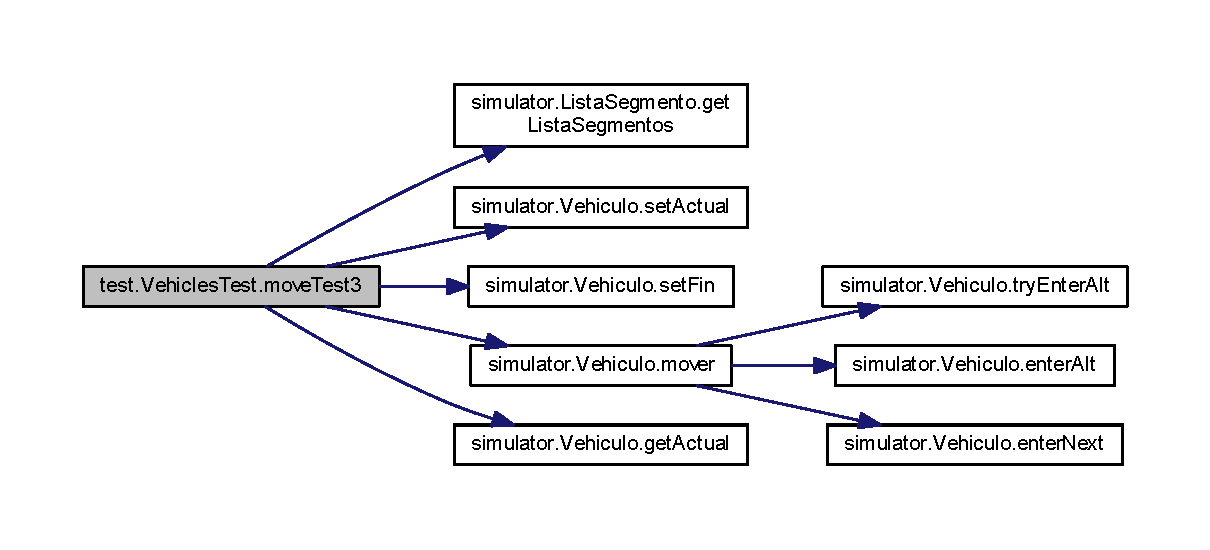
\includegraphics[width=350pt]{classtest_1_1_vehicles_test_ac6267ff4e71ba311e03c25de20196e65_cgraph}
\end{center}
\end{figure}
\mbox{\Hypertarget{classtest_1_1_vehicles_test_acb2d255019e8718669cb5d6105fd43fa}\label{classtest_1_1_vehicles_test_acb2d255019e8718669cb5d6105fd43fa}} 
\index{test\+::\+Vehicles\+Test@{test\+::\+Vehicles\+Test}!move\+Test4@{move\+Test4}}
\index{move\+Test4@{move\+Test4}!test\+::\+Vehicles\+Test@{test\+::\+Vehicles\+Test}}
\subsubsection{\texorpdfstring{move\+Test4()}{moveTest4()}}
{\footnotesize\ttfamily void test.\+Vehicles\+Test.\+move\+Test4 (\begin{DoxyParamCaption}{ }\end{DoxyParamCaption})}



Definition at line 154 of file Vehicles\+Test.\+java.

Here is the call graph for this function\+:\nopagebreak
\begin{figure}[H]
\begin{center}
\leavevmode
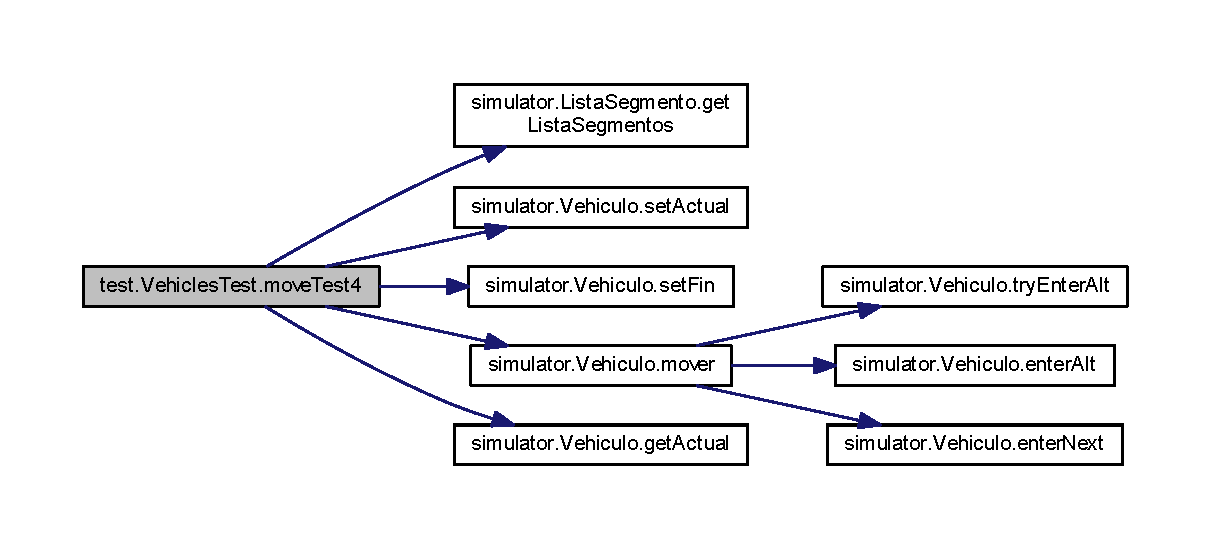
\includegraphics[width=350pt]{classtest_1_1_vehicles_test_acb2d255019e8718669cb5d6105fd43fa_cgraph}
\end{center}
\end{figure}
\mbox{\Hypertarget{classtest_1_1_vehicles_test_a11f99870b0a4caa2075a2bdeaf910523}\label{classtest_1_1_vehicles_test_a11f99870b0a4caa2075a2bdeaf910523}} 
\index{test\+::\+Vehicles\+Test@{test\+::\+Vehicles\+Test}!move\+Test5@{move\+Test5}}
\index{move\+Test5@{move\+Test5}!test\+::\+Vehicles\+Test@{test\+::\+Vehicles\+Test}}
\subsubsection{\texorpdfstring{move\+Test5()}{moveTest5()}}
{\footnotesize\ttfamily void test.\+Vehicles\+Test.\+move\+Test5 (\begin{DoxyParamCaption}{ }\end{DoxyParamCaption})}



Definition at line 165 of file Vehicles\+Test.\+java.

Here is the call graph for this function\+:\nopagebreak
\begin{figure}[H]
\begin{center}
\leavevmode
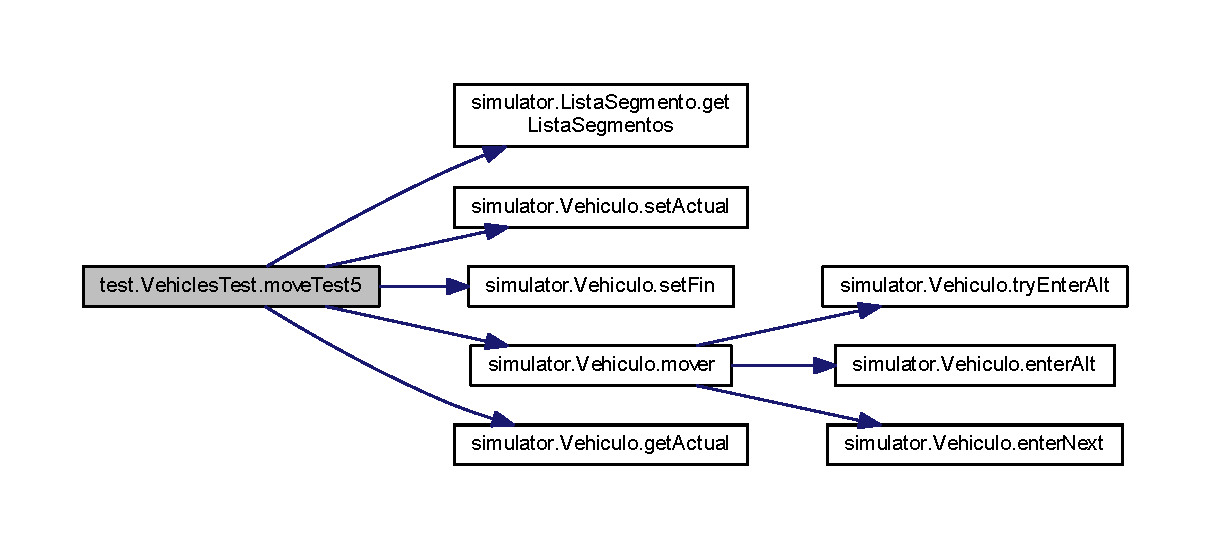
\includegraphics[width=350pt]{classtest_1_1_vehicles_test_a11f99870b0a4caa2075a2bdeaf910523_cgraph}
\end{center}
\end{figure}
\mbox{\Hypertarget{classtest_1_1_vehicles_test_add2a427b283ac60b944e500f0c66e20b}\label{classtest_1_1_vehicles_test_add2a427b283ac60b944e500f0c66e20b}} 
\index{test\+::\+Vehicles\+Test@{test\+::\+Vehicles\+Test}!move\+Test6@{move\+Test6}}
\index{move\+Test6@{move\+Test6}!test\+::\+Vehicles\+Test@{test\+::\+Vehicles\+Test}}
\subsubsection{\texorpdfstring{move\+Test6()}{moveTest6()}}
{\footnotesize\ttfamily void test.\+Vehicles\+Test.\+move\+Test6 (\begin{DoxyParamCaption}{ }\end{DoxyParamCaption})}



Definition at line 176 of file Vehicles\+Test.\+java.

Here is the call graph for this function\+:\nopagebreak
\begin{figure}[H]
\begin{center}
\leavevmode
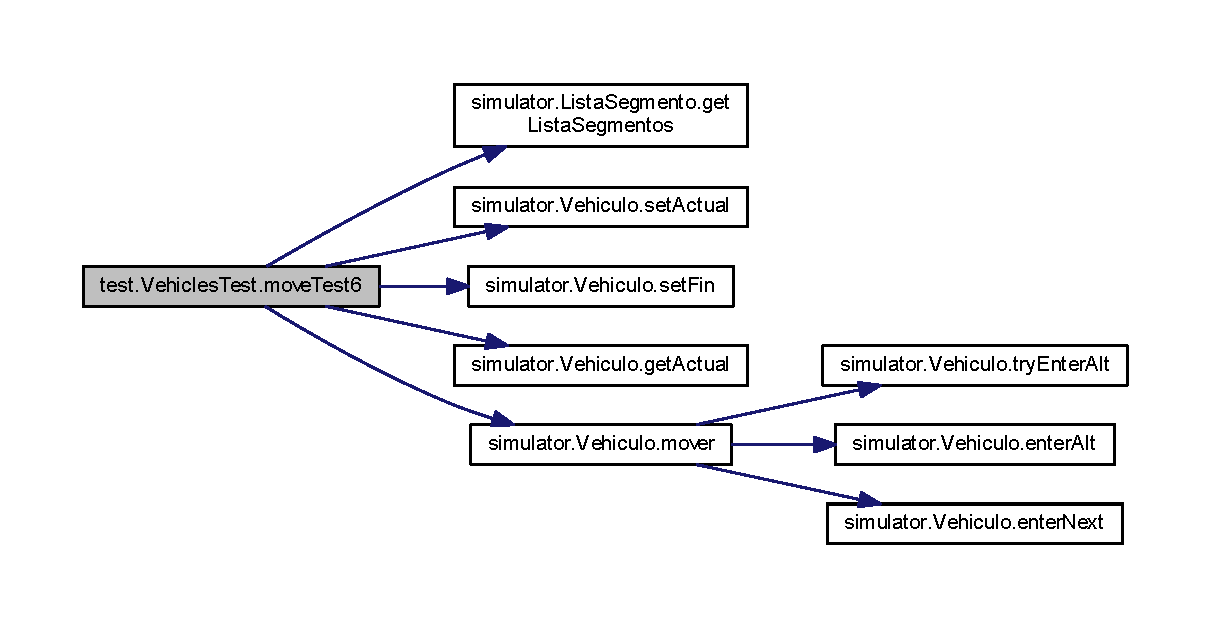
\includegraphics[width=350pt]{classtest_1_1_vehicles_test_add2a427b283ac60b944e500f0c66e20b_cgraph}
\end{center}
\end{figure}
\mbox{\Hypertarget{classtest_1_1_vehicles_test_ac0fe870f7fb0e6bd96317b5e8a9c06d0}\label{classtest_1_1_vehicles_test_ac0fe870f7fb0e6bd96317b5e8a9c06d0}} 
\index{test\+::\+Vehicles\+Test@{test\+::\+Vehicles\+Test}!move\+Test7@{move\+Test7}}
\index{move\+Test7@{move\+Test7}!test\+::\+Vehicles\+Test@{test\+::\+Vehicles\+Test}}
\subsubsection{\texorpdfstring{move\+Test7()}{moveTest7()}}
{\footnotesize\ttfamily void test.\+Vehicles\+Test.\+move\+Test7 (\begin{DoxyParamCaption}{ }\end{DoxyParamCaption})}



Definition at line 188 of file Vehicles\+Test.\+java.

Here is the call graph for this function\+:\nopagebreak
\begin{figure}[H]
\begin{center}
\leavevmode
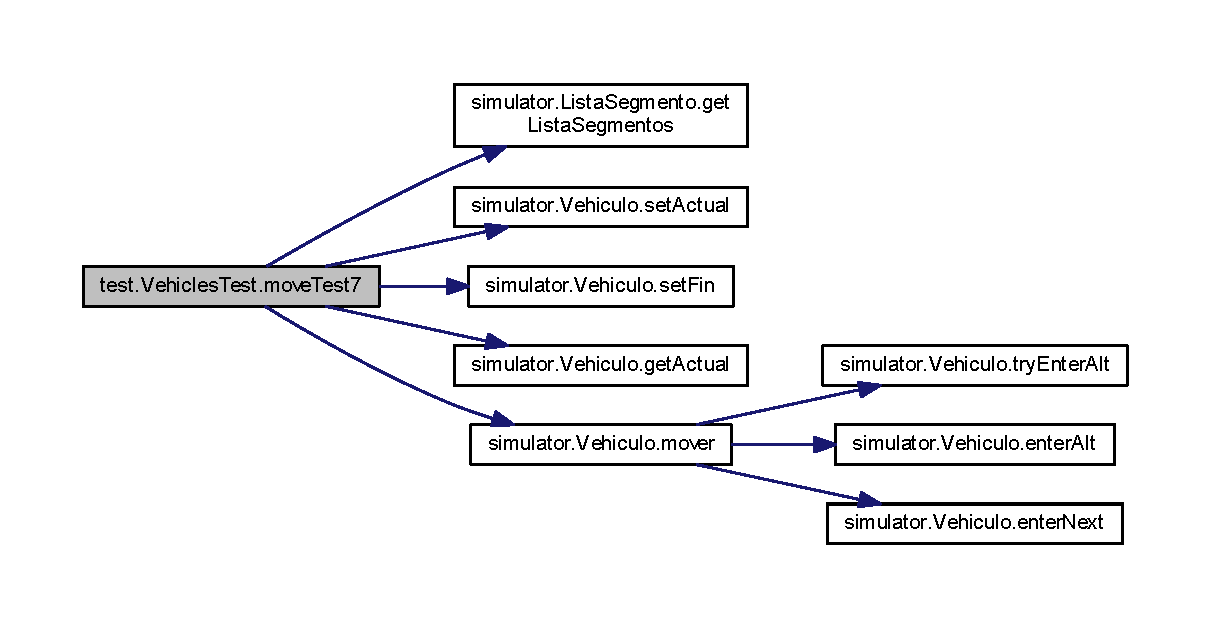
\includegraphics[width=350pt]{classtest_1_1_vehicles_test_ac0fe870f7fb0e6bd96317b5e8a9c06d0_cgraph}
\end{center}
\end{figure}
\mbox{\Hypertarget{classtest_1_1_vehicles_test_ae80a57f1f29cea08685e8f835d0a6d63}\label{classtest_1_1_vehicles_test_ae80a57f1f29cea08685e8f835d0a6d63}} 
\index{test\+::\+Vehicles\+Test@{test\+::\+Vehicles\+Test}!move\+Test8@{move\+Test8}}
\index{move\+Test8@{move\+Test8}!test\+::\+Vehicles\+Test@{test\+::\+Vehicles\+Test}}
\subsubsection{\texorpdfstring{move\+Test8()}{moveTest8()}}
{\footnotesize\ttfamily void test.\+Vehicles\+Test.\+move\+Test8 (\begin{DoxyParamCaption}{ }\end{DoxyParamCaption})}



Definition at line 200 of file Vehicles\+Test.\+java.

Here is the call graph for this function\+:\nopagebreak
\begin{figure}[H]
\begin{center}
\leavevmode
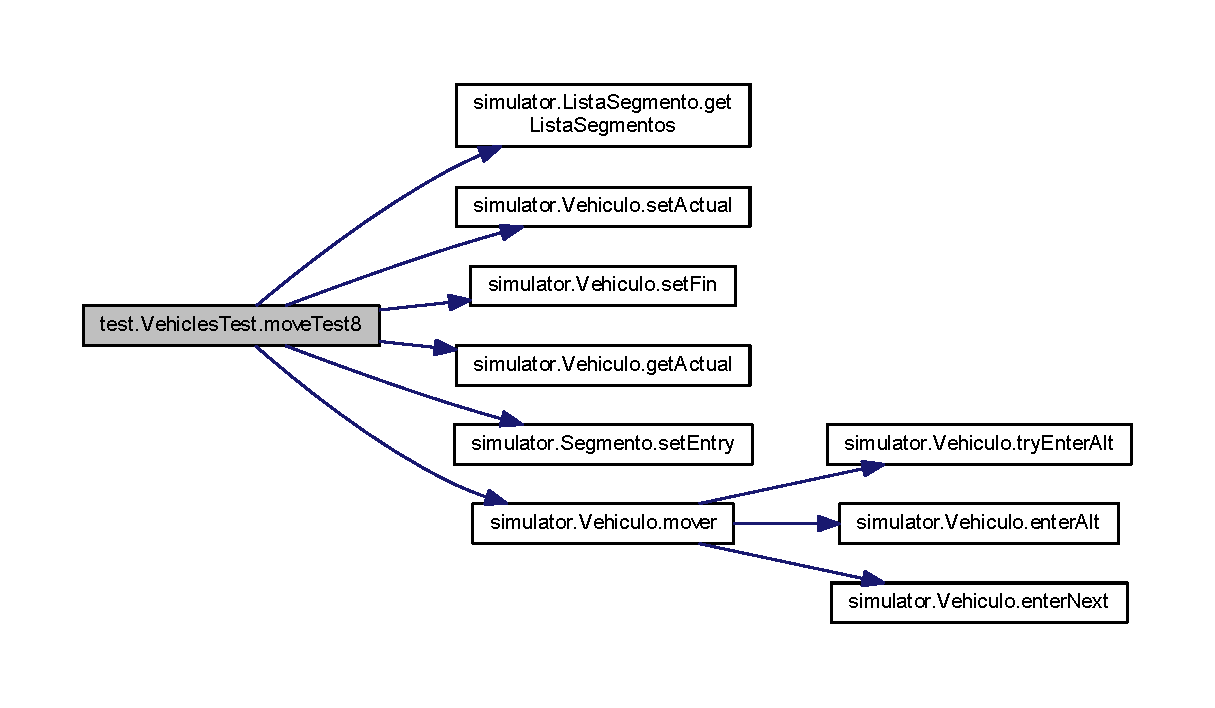
\includegraphics[width=350pt]{classtest_1_1_vehicles_test_ae80a57f1f29cea08685e8f835d0a6d63_cgraph}
\end{center}
\end{figure}
\mbox{\Hypertarget{classtest_1_1_vehicles_test_ae9e8f3b27af5bb2a0d7b7f52da6ba833}\label{classtest_1_1_vehicles_test_ae9e8f3b27af5bb2a0d7b7f52da6ba833}} 
\index{test\+::\+Vehicles\+Test@{test\+::\+Vehicles\+Test}!move\+Test9@{move\+Test9}}
\index{move\+Test9@{move\+Test9}!test\+::\+Vehicles\+Test@{test\+::\+Vehicles\+Test}}
\subsubsection{\texorpdfstring{move\+Test9()}{moveTest9()}}
{\footnotesize\ttfamily void test.\+Vehicles\+Test.\+move\+Test9 (\begin{DoxyParamCaption}{ }\end{DoxyParamCaption})}



Definition at line 213 of file Vehicles\+Test.\+java.

Here is the call graph for this function\+:\nopagebreak
\begin{figure}[H]
\begin{center}
\leavevmode
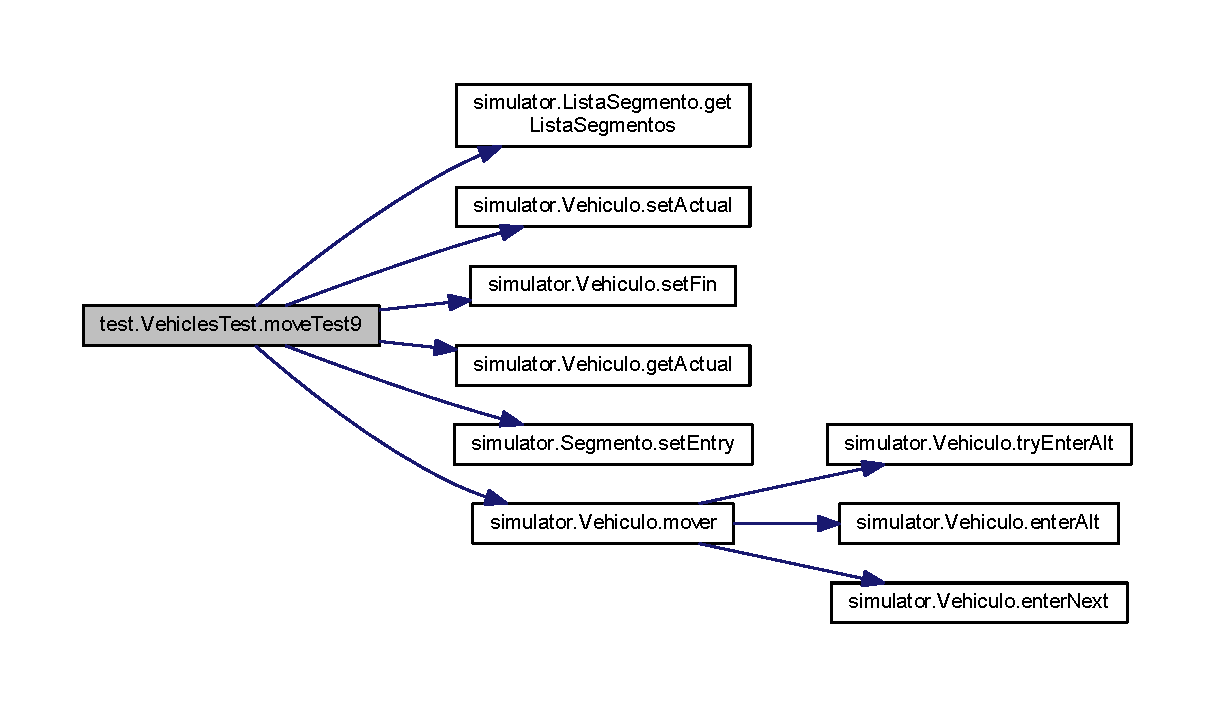
\includegraphics[width=350pt]{classtest_1_1_vehicles_test_ae9e8f3b27af5bb2a0d7b7f52da6ba833_cgraph}
\end{center}
\end{figure}
\mbox{\Hypertarget{classtest_1_1_vehicles_test_a7ff46f63103aef8f984b7fbb1f9857fe}\label{classtest_1_1_vehicles_test_a7ff46f63103aef8f984b7fbb1f9857fe}} 
\index{test\+::\+Vehicles\+Test@{test\+::\+Vehicles\+Test}!try\+Enter\+Alt\+Test@{try\+Enter\+Alt\+Test}}
\index{try\+Enter\+Alt\+Test@{try\+Enter\+Alt\+Test}!test\+::\+Vehicles\+Test@{test\+::\+Vehicles\+Test}}
\subsubsection{\texorpdfstring{try\+Enter\+Alt\+Test()}{tryEnterAltTest()}}
{\footnotesize\ttfamily void test.\+Vehicles\+Test.\+try\+Enter\+Alt\+Test (\begin{DoxyParamCaption}{ }\end{DoxyParamCaption})}



Definition at line 87 of file Vehicles\+Test.\+java.

Here is the call graph for this function\+:\nopagebreak
\begin{figure}[H]
\begin{center}
\leavevmode
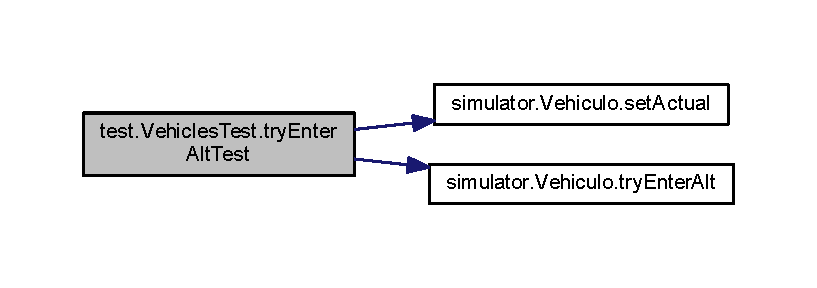
\includegraphics[width=350pt]{classtest_1_1_vehicles_test_a7ff46f63103aef8f984b7fbb1f9857fe_cgraph}
\end{center}
\end{figure}


\subsection{Member Data Documentation}
\mbox{\Hypertarget{classtest_1_1_vehicles_test_aaabf0794cb228d330952cb1392a034b0}\label{classtest_1_1_vehicles_test_aaabf0794cb228d330952cb1392a034b0}} 
\index{test\+::\+Vehicles\+Test@{test\+::\+Vehicles\+Test}!system\+Out\+Rule@{system\+Out\+Rule}}
\index{system\+Out\+Rule@{system\+Out\+Rule}!test\+::\+Vehicles\+Test@{test\+::\+Vehicles\+Test}}
\subsubsection{\texorpdfstring{system\+Out\+Rule}{systemOutRule}}
{\footnotesize\ttfamily final System\+Out\+Rule test.\+Vehicles\+Test.\+system\+Out\+Rule = new System\+Out\+Rule().enable\+Log()}



Definition at line 50 of file Vehicles\+Test.\+java.



The documentation for this class was generated from the following file\+:\begin{DoxyCompactItemize}
\item 
java/test/java/test/\mbox{\hyperlink{_vehicles_test_8java}{Vehicles\+Test.\+java}}\end{DoxyCompactItemize}

\hypertarget{classsimulator_1_1_vehiculo}{}\section{simulator.\+Vehiculo Class Reference}
\label{classsimulator_1_1_vehiculo}\index{simulator.\+Vehiculo@{simulator.\+Vehiculo}}


Inheritance diagram for simulator.\+Vehiculo\+:\nopagebreak
\begin{figure}[H]
\begin{center}
\leavevmode
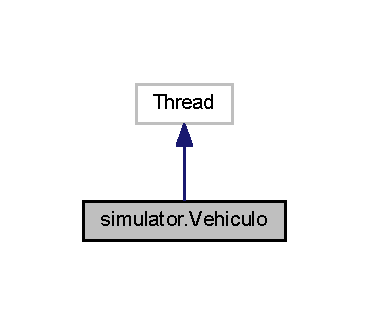
\includegraphics[width=177pt]{classsimulator_1_1_vehiculo__inherit__graph}
\end{center}
\end{figure}


Collaboration diagram for simulator.\+Vehiculo\+:\nopagebreak
\begin{figure}[H]
\begin{center}
\leavevmode
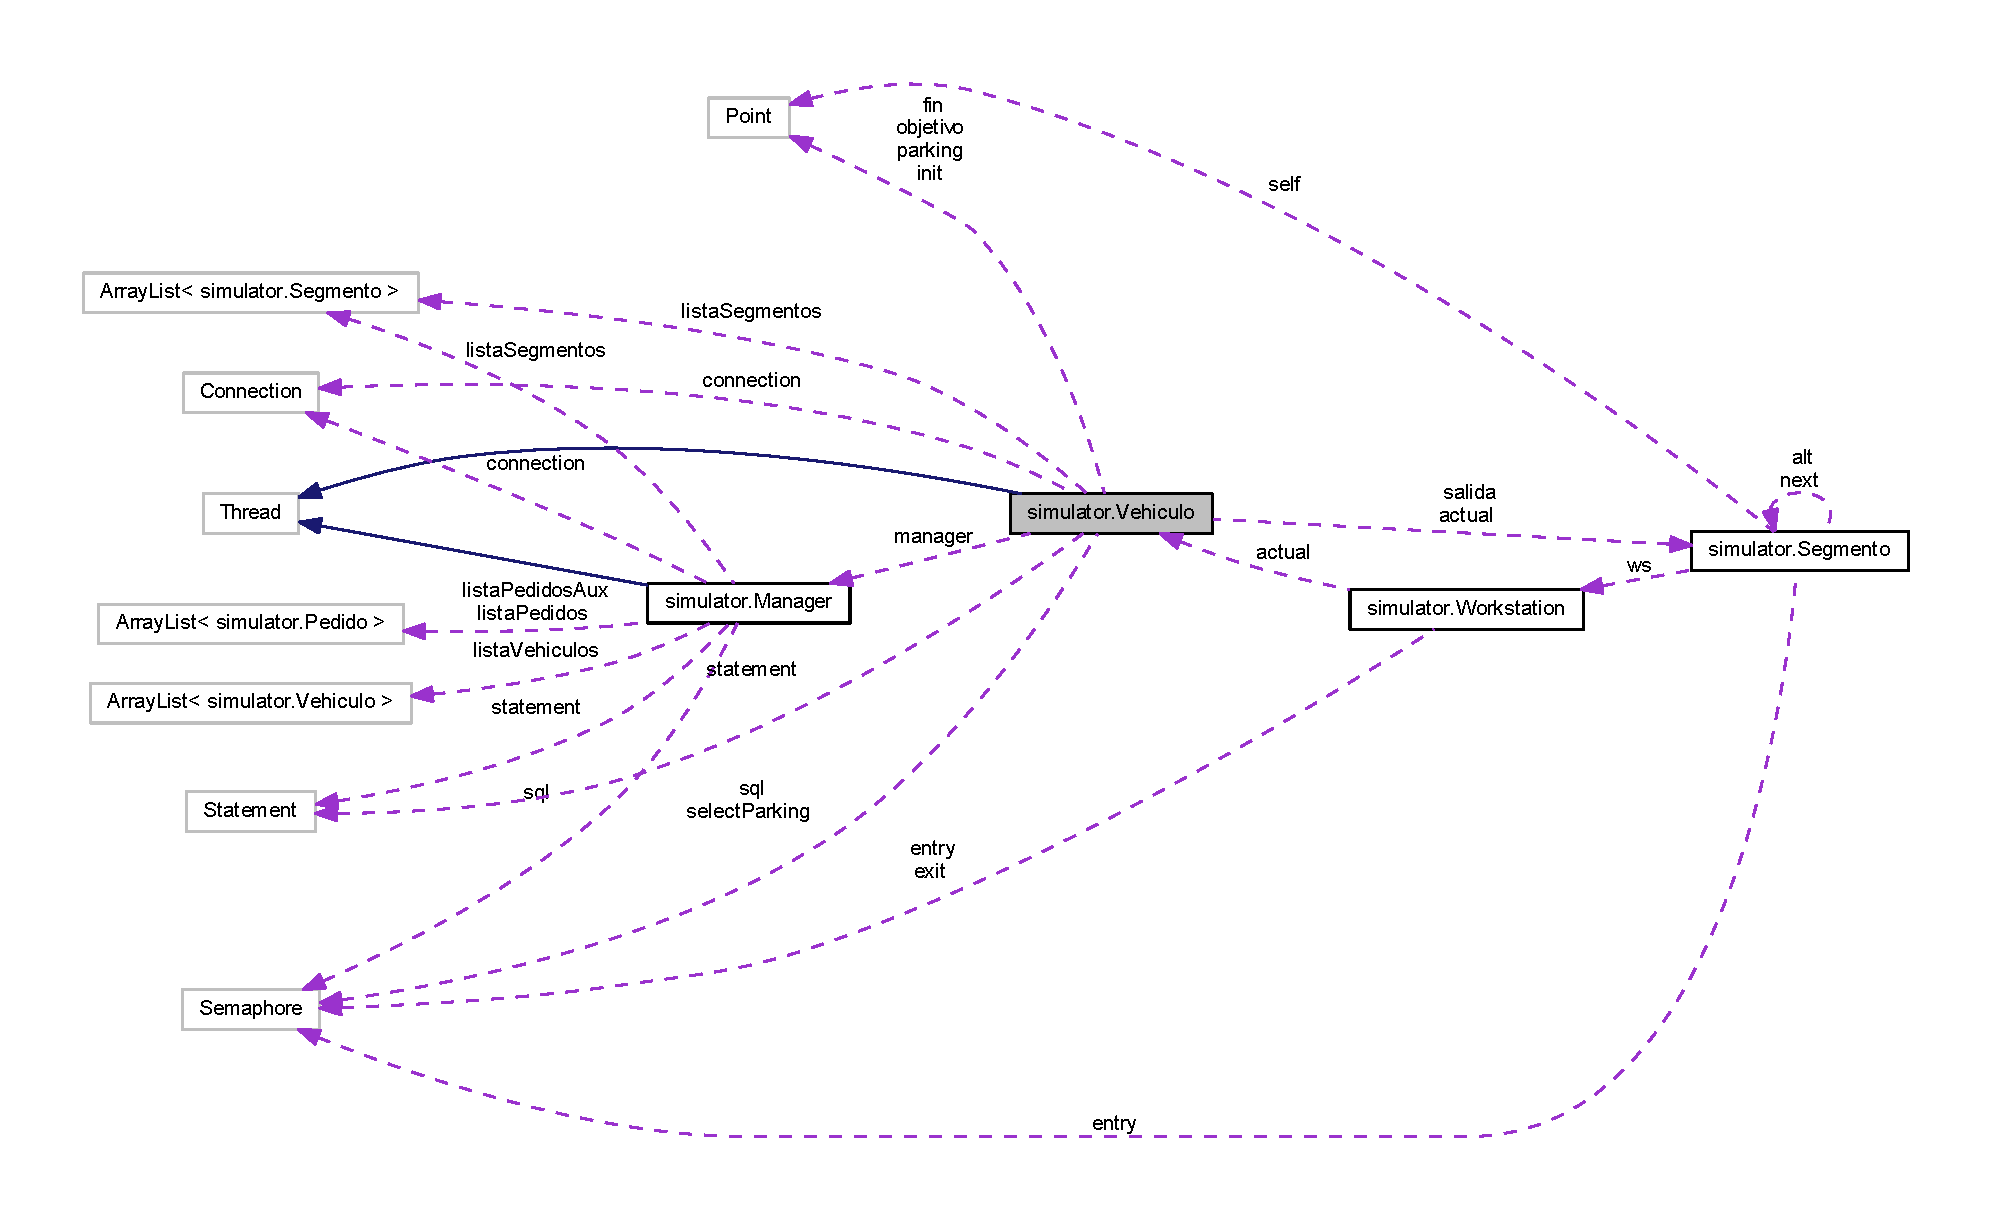
\includegraphics[width=350pt]{classsimulator_1_1_vehiculo__coll__graph}
\end{center}
\end{figure}
\subsection*{Public Member Functions}
\begin{DoxyCompactItemize}
\item 
\mbox{\hyperlink{classsimulator_1_1_vehiculo_a1614333acce021409a3bfe74a88750d4}{Vehiculo}} (Point init, Point fin, Array\+List$<$ \mbox{\hyperlink{classsimulator_1_1_segmento}{Segmento}} $>$ lista\+Segmentos, int id, Semaphore select\+Parking, Semaphore sql, \mbox{\hyperlink{classsimulator_1_1_manager}{Manager}} manager)
\item 
void \mbox{\hyperlink{classsimulator_1_1_vehiculo_a7dc301ce9a868990dea8e406dd038979}{connect}} (String username)
\item 
void \mbox{\hyperlink{classsimulator_1_1_vehiculo_aca90600bc94ce6dd02ddd4e5b712e687}{buscar\+Actual}} ()
\item 
void \mbox{\hyperlink{classsimulator_1_1_vehiculo_aa59295cc134f0db04e5b822ec7d6d147}{buscar\+Parking}} ()
\item 
void \mbox{\hyperlink{classsimulator_1_1_vehiculo_a6180368ea8c35b2e7113a5f2b1368f92}{mover}} ()
\item 
Semaphore \mbox{\hyperlink{classsimulator_1_1_vehiculo_afff145cddc29699082dab8c05d18137d}{get\+Select\+Parking}} ()
\item 
void \mbox{\hyperlink{classsimulator_1_1_vehiculo_aa860fe7afa2700e63751b39296a3dbe2}{entrar\+Parking}} ()
\item 
boolean \mbox{\hyperlink{classsimulator_1_1_vehiculo_a7206f5327c1bb0c7e5ce49d526542740}{llegada}} ()
\item 
void \mbox{\hyperlink{classsimulator_1_1_vehiculo_aa917981d13bea186e4016a9a367c8288}{set\+Producto\+ID}} (int producto\+ID)
\item 
void \mbox{\hyperlink{classsimulator_1_1_vehiculo_ac84b60f19a1fcfa901dc0be573edf80f}{set\+Pedido\+ID}} (int pedido\+ID)
\item 
Semaphore \mbox{\hyperlink{classsimulator_1_1_vehiculo_a5dfc609221e17e725449964f7482b109}{get\+Sql}} ()
\item 
\mbox{\hyperlink{classsimulator_1_1_segmento}{Segmento}} \mbox{\hyperlink{classsimulator_1_1_vehiculo_ad3da0b0e11fbf762c9efbc02af14791a}{get\+Salida}} ()
\item 
Point \mbox{\hyperlink{classsimulator_1_1_vehiculo_a12c1abc60bddb033fdd3e04f14bb8314}{get\+Objetivo}} ()
\item 
void \mbox{\hyperlink{classsimulator_1_1_vehiculo_a1eb291b75826b406fc1eee91a92b9653}{set\+Objetivo}} (Point objetivo)
\item 
void \mbox{\hyperlink{classsimulator_1_1_vehiculo_a4cbe0a3d742c02919a0c355f42f3e35d}{run}} ()
\item 
boolean \mbox{\hyperlink{classsimulator_1_1_vehiculo_a74f78a4942efa75589834e4ad4e95fc4}{try\+Enter\+Alt}} ()
\item 
void \mbox{\hyperlink{classsimulator_1_1_vehiculo_aee3cf4905b7d3668f705d8bab550cf78}{enter\+Alt}} ()
\item 
void \mbox{\hyperlink{classsimulator_1_1_vehiculo_ae2109a07a4719805b2b22fa2cfc74b9b}{enter\+Next}} ()
\item 
\mbox{\hyperlink{classsimulator_1_1_segmento}{Segmento}} \mbox{\hyperlink{classsimulator_1_1_vehiculo_ad6305ffaaa4eee022c07cac7515df015}{get\+Actual}} ()
\item 
Point \mbox{\hyperlink{classsimulator_1_1_vehiculo_a4adff38665fbd605cc1aadf42dae9787}{get\+Fin}} ()
\item 
void \mbox{\hyperlink{classsimulator_1_1_vehiculo_ac31a172023d50e9ac576ffb0f449bfb8}{set\+Fin}} (Point fin)
\item 
void \mbox{\hyperlink{classsimulator_1_1_vehiculo_a2515527cf1b20dfbd634f6bc54e3f8ad}{set\+Parking}} (Point point)
\item 
void \mbox{\hyperlink{classsimulator_1_1_vehiculo_ae8246a5b77441c21681ffd2033075348}{set\+Actual}} (\mbox{\hyperlink{classsimulator_1_1_segmento}{Segmento}} segmento)
\end{DoxyCompactItemize}


\subsection{Detailed Description}
This is the Vehicle class. Vehicle

\begin{DoxyAuthor}{Author}
Joseba Carnicero, Aitor Eizmendi, Jon Mugica and Marcos Azkarate 
\end{DoxyAuthor}


Definition at line 19 of file Vehiculo.\+java.



\subsection{Constructor \& Destructor Documentation}
\mbox{\Hypertarget{classsimulator_1_1_vehiculo_a1614333acce021409a3bfe74a88750d4}\label{classsimulator_1_1_vehiculo_a1614333acce021409a3bfe74a88750d4}} 
\index{simulator\+::\+Vehiculo@{simulator\+::\+Vehiculo}!Vehiculo@{Vehiculo}}
\index{Vehiculo@{Vehiculo}!simulator\+::\+Vehiculo@{simulator\+::\+Vehiculo}}
\subsubsection{\texorpdfstring{Vehiculo()}{Vehiculo()}}
{\footnotesize\ttfamily simulator.\+Vehiculo.\+Vehiculo (\begin{DoxyParamCaption}\item[{Point}]{init,  }\item[{Point}]{fin,  }\item[{Array\+List$<$ \mbox{\hyperlink{classsimulator_1_1_segmento}{Segmento}} $>$}]{lista\+Segmentos,  }\item[{int}]{id,  }\item[{Semaphore}]{select\+Parking,  }\item[{Semaphore}]{sql,  }\item[{\mbox{\hyperlink{classsimulator_1_1_manager}{Manager}}}]{manager }\end{DoxyParamCaption})}



Definition at line 47 of file Vehiculo.\+java.

Here is the call graph for this function\+:\nopagebreak
\begin{figure}[H]
\begin{center}
\leavevmode
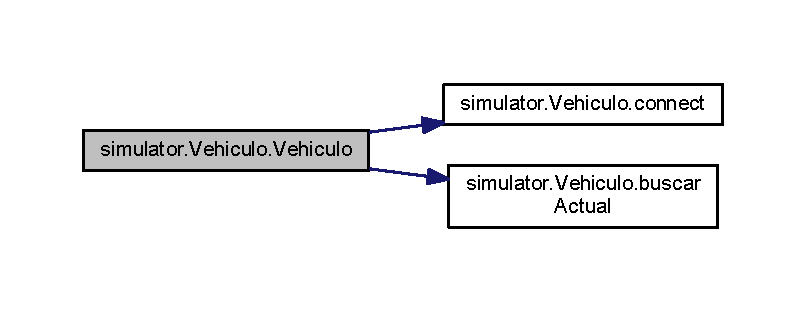
\includegraphics[width=350pt]{classsimulator_1_1_vehiculo_a1614333acce021409a3bfe74a88750d4_cgraph}
\end{center}
\end{figure}


\subsection{Member Function Documentation}
\mbox{\Hypertarget{classsimulator_1_1_vehiculo_aca90600bc94ce6dd02ddd4e5b712e687}\label{classsimulator_1_1_vehiculo_aca90600bc94ce6dd02ddd4e5b712e687}} 
\index{simulator\+::\+Vehiculo@{simulator\+::\+Vehiculo}!buscar\+Actual@{buscar\+Actual}}
\index{buscar\+Actual@{buscar\+Actual}!simulator\+::\+Vehiculo@{simulator\+::\+Vehiculo}}
\subsubsection{\texorpdfstring{buscar\+Actual()}{buscarActual()}}
{\footnotesize\ttfamily void simulator.\+Vehiculo.\+buscar\+Actual (\begin{DoxyParamCaption}{ }\end{DoxyParamCaption})}

This method reserve an segment to a certain vehicle 

Definition at line 88 of file Vehiculo.\+java.

\mbox{\Hypertarget{classsimulator_1_1_vehiculo_aa59295cc134f0db04e5b822ec7d6d147}\label{classsimulator_1_1_vehiculo_aa59295cc134f0db04e5b822ec7d6d147}} 
\index{simulator\+::\+Vehiculo@{simulator\+::\+Vehiculo}!buscar\+Parking@{buscar\+Parking}}
\index{buscar\+Parking@{buscar\+Parking}!simulator\+::\+Vehiculo@{simulator\+::\+Vehiculo}}
\subsubsection{\texorpdfstring{buscar\+Parking()}{buscarParking()}}
{\footnotesize\ttfamily void simulator.\+Vehiculo.\+buscar\+Parking (\begin{DoxyParamCaption}{ }\end{DoxyParamCaption})}

This method look for a parking segment. 

Definition at line 109 of file Vehiculo.\+java.

\mbox{\Hypertarget{classsimulator_1_1_vehiculo_a7dc301ce9a868990dea8e406dd038979}\label{classsimulator_1_1_vehiculo_a7dc301ce9a868990dea8e406dd038979}} 
\index{simulator\+::\+Vehiculo@{simulator\+::\+Vehiculo}!connect@{connect}}
\index{connect@{connect}!simulator\+::\+Vehiculo@{simulator\+::\+Vehiculo}}
\subsubsection{\texorpdfstring{connect()}{connect()}}
{\footnotesize\ttfamily void simulator.\+Vehiculo.\+connect (\begin{DoxyParamCaption}\item[{String}]{username }\end{DoxyParamCaption})}

This method connects to the selected database 

Definition at line 66 of file Vehiculo.\+java.

\mbox{\Hypertarget{classsimulator_1_1_vehiculo_aee3cf4905b7d3668f705d8bab550cf78}\label{classsimulator_1_1_vehiculo_aee3cf4905b7d3668f705d8bab550cf78}} 
\index{simulator\+::\+Vehiculo@{simulator\+::\+Vehiculo}!enter\+Alt@{enter\+Alt}}
\index{enter\+Alt@{enter\+Alt}!simulator\+::\+Vehiculo@{simulator\+::\+Vehiculo}}
\subsubsection{\texorpdfstring{enter\+Alt()}{enterAlt()}}
{\footnotesize\ttfamily void simulator.\+Vehiculo.\+enter\+Alt (\begin{DoxyParamCaption}{ }\end{DoxyParamCaption})}

This method simulates the entrance of a vehicle into a vertical segment 

Definition at line 359 of file Vehiculo.\+java.

\mbox{\Hypertarget{classsimulator_1_1_vehiculo_ae2109a07a4719805b2b22fa2cfc74b9b}\label{classsimulator_1_1_vehiculo_ae2109a07a4719805b2b22fa2cfc74b9b}} 
\index{simulator\+::\+Vehiculo@{simulator\+::\+Vehiculo}!enter\+Next@{enter\+Next}}
\index{enter\+Next@{enter\+Next}!simulator\+::\+Vehiculo@{simulator\+::\+Vehiculo}}
\subsubsection{\texorpdfstring{enter\+Next()}{enterNext()}}
{\footnotesize\ttfamily void simulator.\+Vehiculo.\+enter\+Next (\begin{DoxyParamCaption}{ }\end{DoxyParamCaption})}

This method simulates the entrance of the vehicle into a horizontal segment 

Definition at line 405 of file Vehiculo.\+java.

\mbox{\Hypertarget{classsimulator_1_1_vehiculo_aa860fe7afa2700e63751b39296a3dbe2}\label{classsimulator_1_1_vehiculo_aa860fe7afa2700e63751b39296a3dbe2}} 
\index{simulator\+::\+Vehiculo@{simulator\+::\+Vehiculo}!entrar\+Parking@{entrar\+Parking}}
\index{entrar\+Parking@{entrar\+Parking}!simulator\+::\+Vehiculo@{simulator\+::\+Vehiculo}}
\subsubsection{\texorpdfstring{entrar\+Parking()}{entrarParking()}}
{\footnotesize\ttfamily void simulator.\+Vehiculo.\+entrar\+Parking (\begin{DoxyParamCaption}{ }\end{DoxyParamCaption})}

This method simulates the entry into a parking 

Definition at line 180 of file Vehiculo.\+java.

\mbox{\Hypertarget{classsimulator_1_1_vehiculo_ad6305ffaaa4eee022c07cac7515df015}\label{classsimulator_1_1_vehiculo_ad6305ffaaa4eee022c07cac7515df015}} 
\index{simulator\+::\+Vehiculo@{simulator\+::\+Vehiculo}!get\+Actual@{get\+Actual}}
\index{get\+Actual@{get\+Actual}!simulator\+::\+Vehiculo@{simulator\+::\+Vehiculo}}
\subsubsection{\texorpdfstring{get\+Actual()}{getActual()}}
{\footnotesize\ttfamily \mbox{\hyperlink{classsimulator_1_1_segmento}{Segmento}} simulator.\+Vehiculo.\+get\+Actual (\begin{DoxyParamCaption}{ }\end{DoxyParamCaption})}



Definition at line 454 of file Vehiculo.\+java.

\mbox{\Hypertarget{classsimulator_1_1_vehiculo_a4adff38665fbd605cc1aadf42dae9787}\label{classsimulator_1_1_vehiculo_a4adff38665fbd605cc1aadf42dae9787}} 
\index{simulator\+::\+Vehiculo@{simulator\+::\+Vehiculo}!get\+Fin@{get\+Fin}}
\index{get\+Fin@{get\+Fin}!simulator\+::\+Vehiculo@{simulator\+::\+Vehiculo}}
\subsubsection{\texorpdfstring{get\+Fin()}{getFin()}}
{\footnotesize\ttfamily Point simulator.\+Vehiculo.\+get\+Fin (\begin{DoxyParamCaption}{ }\end{DoxyParamCaption})}



Definition at line 459 of file Vehiculo.\+java.

\mbox{\Hypertarget{classsimulator_1_1_vehiculo_a12c1abc60bddb033fdd3e04f14bb8314}\label{classsimulator_1_1_vehiculo_a12c1abc60bddb033fdd3e04f14bb8314}} 
\index{simulator\+::\+Vehiculo@{simulator\+::\+Vehiculo}!get\+Objetivo@{get\+Objetivo}}
\index{get\+Objetivo@{get\+Objetivo}!simulator\+::\+Vehiculo@{simulator\+::\+Vehiculo}}
\subsubsection{\texorpdfstring{get\+Objetivo()}{getObjetivo()}}
{\footnotesize\ttfamily Point simulator.\+Vehiculo.\+get\+Objetivo (\begin{DoxyParamCaption}{ }\end{DoxyParamCaption})}



Definition at line 310 of file Vehiculo.\+java.

\mbox{\Hypertarget{classsimulator_1_1_vehiculo_ad3da0b0e11fbf762c9efbc02af14791a}\label{classsimulator_1_1_vehiculo_ad3da0b0e11fbf762c9efbc02af14791a}} 
\index{simulator\+::\+Vehiculo@{simulator\+::\+Vehiculo}!get\+Salida@{get\+Salida}}
\index{get\+Salida@{get\+Salida}!simulator\+::\+Vehiculo@{simulator\+::\+Vehiculo}}
\subsubsection{\texorpdfstring{get\+Salida()}{getSalida()}}
{\footnotesize\ttfamily \mbox{\hyperlink{classsimulator_1_1_segmento}{Segmento}} simulator.\+Vehiculo.\+get\+Salida (\begin{DoxyParamCaption}{ }\end{DoxyParamCaption})}



Definition at line 306 of file Vehiculo.\+java.

\mbox{\Hypertarget{classsimulator_1_1_vehiculo_afff145cddc29699082dab8c05d18137d}\label{classsimulator_1_1_vehiculo_afff145cddc29699082dab8c05d18137d}} 
\index{simulator\+::\+Vehiculo@{simulator\+::\+Vehiculo}!get\+Select\+Parking@{get\+Select\+Parking}}
\index{get\+Select\+Parking@{get\+Select\+Parking}!simulator\+::\+Vehiculo@{simulator\+::\+Vehiculo}}
\subsubsection{\texorpdfstring{get\+Select\+Parking()}{getSelectParking()}}
{\footnotesize\ttfamily Semaphore simulator.\+Vehiculo.\+get\+Select\+Parking (\begin{DoxyParamCaption}{ }\end{DoxyParamCaption})}



Definition at line 173 of file Vehiculo.\+java.

\mbox{\Hypertarget{classsimulator_1_1_vehiculo_a5dfc609221e17e725449964f7482b109}\label{classsimulator_1_1_vehiculo_a5dfc609221e17e725449964f7482b109}} 
\index{simulator\+::\+Vehiculo@{simulator\+::\+Vehiculo}!get\+Sql@{get\+Sql}}
\index{get\+Sql@{get\+Sql}!simulator\+::\+Vehiculo@{simulator\+::\+Vehiculo}}
\subsubsection{\texorpdfstring{get\+Sql()}{getSql()}}
{\footnotesize\ttfamily Semaphore simulator.\+Vehiculo.\+get\+Sql (\begin{DoxyParamCaption}{ }\end{DoxyParamCaption})}



Definition at line 302 of file Vehiculo.\+java.

\mbox{\Hypertarget{classsimulator_1_1_vehiculo_a7206f5327c1bb0c7e5ce49d526542740}\label{classsimulator_1_1_vehiculo_a7206f5327c1bb0c7e5ce49d526542740}} 
\index{simulator\+::\+Vehiculo@{simulator\+::\+Vehiculo}!llegada@{llegada}}
\index{llegada@{llegada}!simulator\+::\+Vehiculo@{simulator\+::\+Vehiculo}}
\subsubsection{\texorpdfstring{llegada()}{llegada()}}
{\footnotesize\ttfamily boolean simulator.\+Vehiculo.\+llegada (\begin{DoxyParamCaption}{ }\end{DoxyParamCaption})}

\begin{DoxyReturn}{Returns}
true if the vehicle arrives to the final destiny 
\end{DoxyReturn}


Definition at line 209 of file Vehiculo.\+java.

Here is the call graph for this function\+:\nopagebreak
\begin{figure}[H]
\begin{center}
\leavevmode
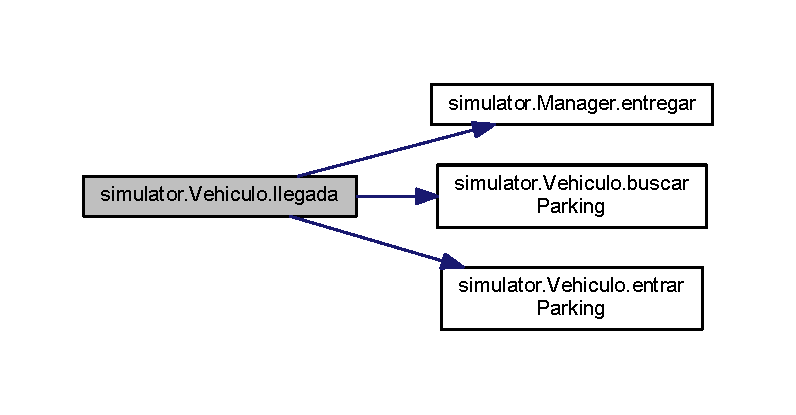
\includegraphics[width=350pt]{classsimulator_1_1_vehiculo_a7206f5327c1bb0c7e5ce49d526542740_cgraph}
\end{center}
\end{figure}
\mbox{\Hypertarget{classsimulator_1_1_vehiculo_a6180368ea8c35b2e7113a5f2b1368f92}\label{classsimulator_1_1_vehiculo_a6180368ea8c35b2e7113a5f2b1368f92}} 
\index{simulator\+::\+Vehiculo@{simulator\+::\+Vehiculo}!mover@{mover}}
\index{mover@{mover}!simulator\+::\+Vehiculo@{simulator\+::\+Vehiculo}}
\subsubsection{\texorpdfstring{mover()}{mover()}}
{\footnotesize\ttfamily void simulator.\+Vehiculo.\+mover (\begin{DoxyParamCaption}{ }\end{DoxyParamCaption})}

This method simulates the movement of the vehicles 

Definition at line 137 of file Vehiculo.\+java.

Here is the call graph for this function\+:\nopagebreak
\begin{figure}[H]
\begin{center}
\leavevmode
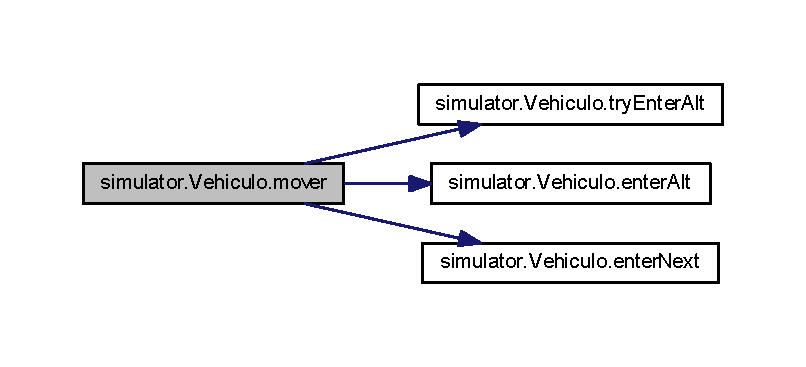
\includegraphics[width=350pt]{classsimulator_1_1_vehiculo_a6180368ea8c35b2e7113a5f2b1368f92_cgraph}
\end{center}
\end{figure}
\mbox{\Hypertarget{classsimulator_1_1_vehiculo_a4cbe0a3d742c02919a0c355f42f3e35d}\label{classsimulator_1_1_vehiculo_a4cbe0a3d742c02919a0c355f42f3e35d}} 
\index{simulator\+::\+Vehiculo@{simulator\+::\+Vehiculo}!run@{run}}
\index{run@{run}!simulator\+::\+Vehiculo@{simulator\+::\+Vehiculo}}
\subsubsection{\texorpdfstring{run()}{run()}}
{\footnotesize\ttfamily void simulator.\+Vehiculo.\+run (\begin{DoxyParamCaption}{ }\end{DoxyParamCaption})}

This method is a loop of 0.\+1 seconds where if the vehicle arrives to the final objective it executes the arrival() function otherwise it will execute move() function 

Definition at line 322 of file Vehiculo.\+java.

Here is the call graph for this function\+:\nopagebreak
\begin{figure}[H]
\begin{center}
\leavevmode
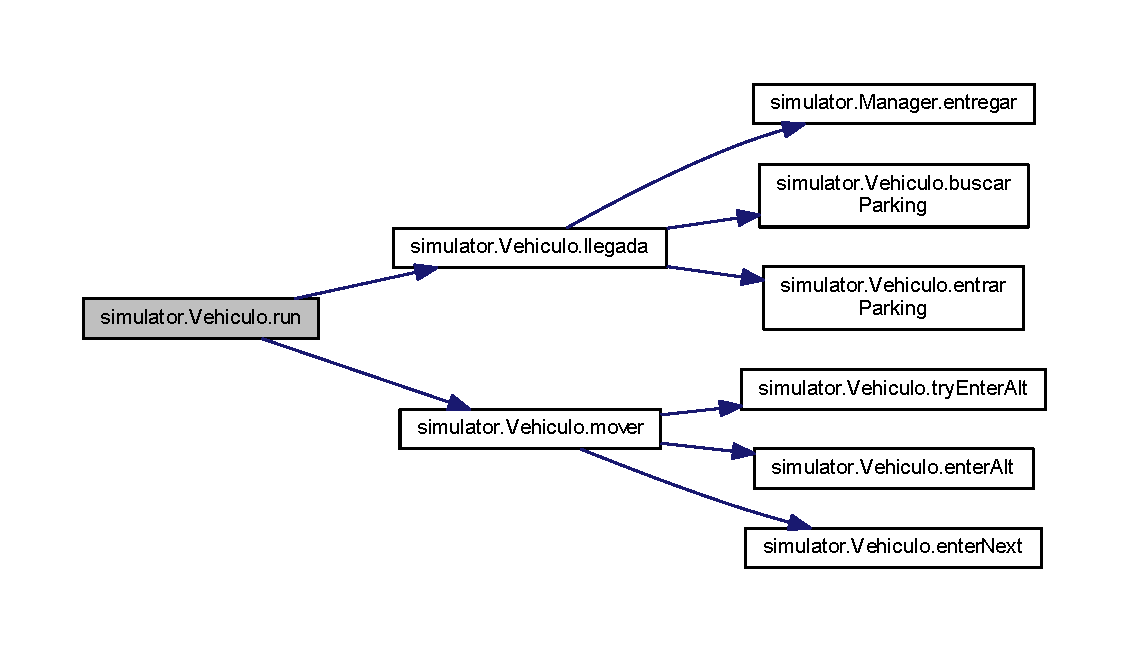
\includegraphics[width=350pt]{classsimulator_1_1_vehiculo_a4cbe0a3d742c02919a0c355f42f3e35d_cgraph}
\end{center}
\end{figure}
\mbox{\Hypertarget{classsimulator_1_1_vehiculo_ae8246a5b77441c21681ffd2033075348}\label{classsimulator_1_1_vehiculo_ae8246a5b77441c21681ffd2033075348}} 
\index{simulator\+::\+Vehiculo@{simulator\+::\+Vehiculo}!set\+Actual@{set\+Actual}}
\index{set\+Actual@{set\+Actual}!simulator\+::\+Vehiculo@{simulator\+::\+Vehiculo}}
\subsubsection{\texorpdfstring{set\+Actual()}{setActual()}}
{\footnotesize\ttfamily void simulator.\+Vehiculo.\+set\+Actual (\begin{DoxyParamCaption}\item[{\mbox{\hyperlink{classsimulator_1_1_segmento}{Segmento}}}]{segmento }\end{DoxyParamCaption})}



Definition at line 472 of file Vehiculo.\+java.

\mbox{\Hypertarget{classsimulator_1_1_vehiculo_ac31a172023d50e9ac576ffb0f449bfb8}\label{classsimulator_1_1_vehiculo_ac31a172023d50e9ac576ffb0f449bfb8}} 
\index{simulator\+::\+Vehiculo@{simulator\+::\+Vehiculo}!set\+Fin@{set\+Fin}}
\index{set\+Fin@{set\+Fin}!simulator\+::\+Vehiculo@{simulator\+::\+Vehiculo}}
\subsubsection{\texorpdfstring{set\+Fin()}{setFin()}}
{\footnotesize\ttfamily void simulator.\+Vehiculo.\+set\+Fin (\begin{DoxyParamCaption}\item[{Point}]{fin }\end{DoxyParamCaption})}



Definition at line 463 of file Vehiculo.\+java.

\mbox{\Hypertarget{classsimulator_1_1_vehiculo_a1eb291b75826b406fc1eee91a92b9653}\label{classsimulator_1_1_vehiculo_a1eb291b75826b406fc1eee91a92b9653}} 
\index{simulator\+::\+Vehiculo@{simulator\+::\+Vehiculo}!set\+Objetivo@{set\+Objetivo}}
\index{set\+Objetivo@{set\+Objetivo}!simulator\+::\+Vehiculo@{simulator\+::\+Vehiculo}}
\subsubsection{\texorpdfstring{set\+Objetivo()}{setObjetivo()}}
{\footnotesize\ttfamily void simulator.\+Vehiculo.\+set\+Objetivo (\begin{DoxyParamCaption}\item[{Point}]{objetivo }\end{DoxyParamCaption})}



Definition at line 314 of file Vehiculo.\+java.

\mbox{\Hypertarget{classsimulator_1_1_vehiculo_a2515527cf1b20dfbd634f6bc54e3f8ad}\label{classsimulator_1_1_vehiculo_a2515527cf1b20dfbd634f6bc54e3f8ad}} 
\index{simulator\+::\+Vehiculo@{simulator\+::\+Vehiculo}!set\+Parking@{set\+Parking}}
\index{set\+Parking@{set\+Parking}!simulator\+::\+Vehiculo@{simulator\+::\+Vehiculo}}
\subsubsection{\texorpdfstring{set\+Parking()}{setParking()}}
{\footnotesize\ttfamily void simulator.\+Vehiculo.\+set\+Parking (\begin{DoxyParamCaption}\item[{Point}]{point }\end{DoxyParamCaption})}



Definition at line 467 of file Vehiculo.\+java.

\mbox{\Hypertarget{classsimulator_1_1_vehiculo_ac84b60f19a1fcfa901dc0be573edf80f}\label{classsimulator_1_1_vehiculo_ac84b60f19a1fcfa901dc0be573edf80f}} 
\index{simulator\+::\+Vehiculo@{simulator\+::\+Vehiculo}!set\+Pedido\+ID@{set\+Pedido\+ID}}
\index{set\+Pedido\+ID@{set\+Pedido\+ID}!simulator\+::\+Vehiculo@{simulator\+::\+Vehiculo}}
\subsubsection{\texorpdfstring{set\+Pedido\+I\+D()}{setPedidoID()}}
{\footnotesize\ttfamily void simulator.\+Vehiculo.\+set\+Pedido\+ID (\begin{DoxyParamCaption}\item[{int}]{pedido\+ID }\end{DoxyParamCaption})}



Definition at line 298 of file Vehiculo.\+java.

\mbox{\Hypertarget{classsimulator_1_1_vehiculo_aa917981d13bea186e4016a9a367c8288}\label{classsimulator_1_1_vehiculo_aa917981d13bea186e4016a9a367c8288}} 
\index{simulator\+::\+Vehiculo@{simulator\+::\+Vehiculo}!set\+Producto\+ID@{set\+Producto\+ID}}
\index{set\+Producto\+ID@{set\+Producto\+ID}!simulator\+::\+Vehiculo@{simulator\+::\+Vehiculo}}
\subsubsection{\texorpdfstring{set\+Producto\+I\+D()}{setProductoID()}}
{\footnotesize\ttfamily void simulator.\+Vehiculo.\+set\+Producto\+ID (\begin{DoxyParamCaption}\item[{int}]{producto\+ID }\end{DoxyParamCaption})}



Definition at line 294 of file Vehiculo.\+java.

\mbox{\Hypertarget{classsimulator_1_1_vehiculo_a74f78a4942efa75589834e4ad4e95fc4}\label{classsimulator_1_1_vehiculo_a74f78a4942efa75589834e4ad4e95fc4}} 
\index{simulator\+::\+Vehiculo@{simulator\+::\+Vehiculo}!try\+Enter\+Alt@{try\+Enter\+Alt}}
\index{try\+Enter\+Alt@{try\+Enter\+Alt}!simulator\+::\+Vehiculo@{simulator\+::\+Vehiculo}}
\subsubsection{\texorpdfstring{try\+Enter\+Alt()}{tryEnterAlt()}}
{\footnotesize\ttfamily boolean simulator.\+Vehiculo.\+try\+Enter\+Alt (\begin{DoxyParamCaption}{ }\end{DoxyParamCaption})}

\begin{DoxyReturn}{Returns}
true if the vertical segment is available, otherwise it will return false 
\end{DoxyReturn}


Definition at line 344 of file Vehiculo.\+java.



The documentation for this class was generated from the following file\+:\begin{DoxyCompactItemize}
\item 
java/main/java/simulator/\mbox{\hyperlink{_vehiculo_8java}{Vehiculo.\+java}}\end{DoxyCompactItemize}

\hypertarget{classsimulator_1_1_workstation}{}\section{simulator.\+Workstation Class Reference}
\label{classsimulator_1_1_workstation}\index{simulator.\+Workstation@{simulator.\+Workstation}}


Collaboration diagram for simulator.\+Workstation\+:\nopagebreak
\begin{figure}[H]
\begin{center}
\leavevmode
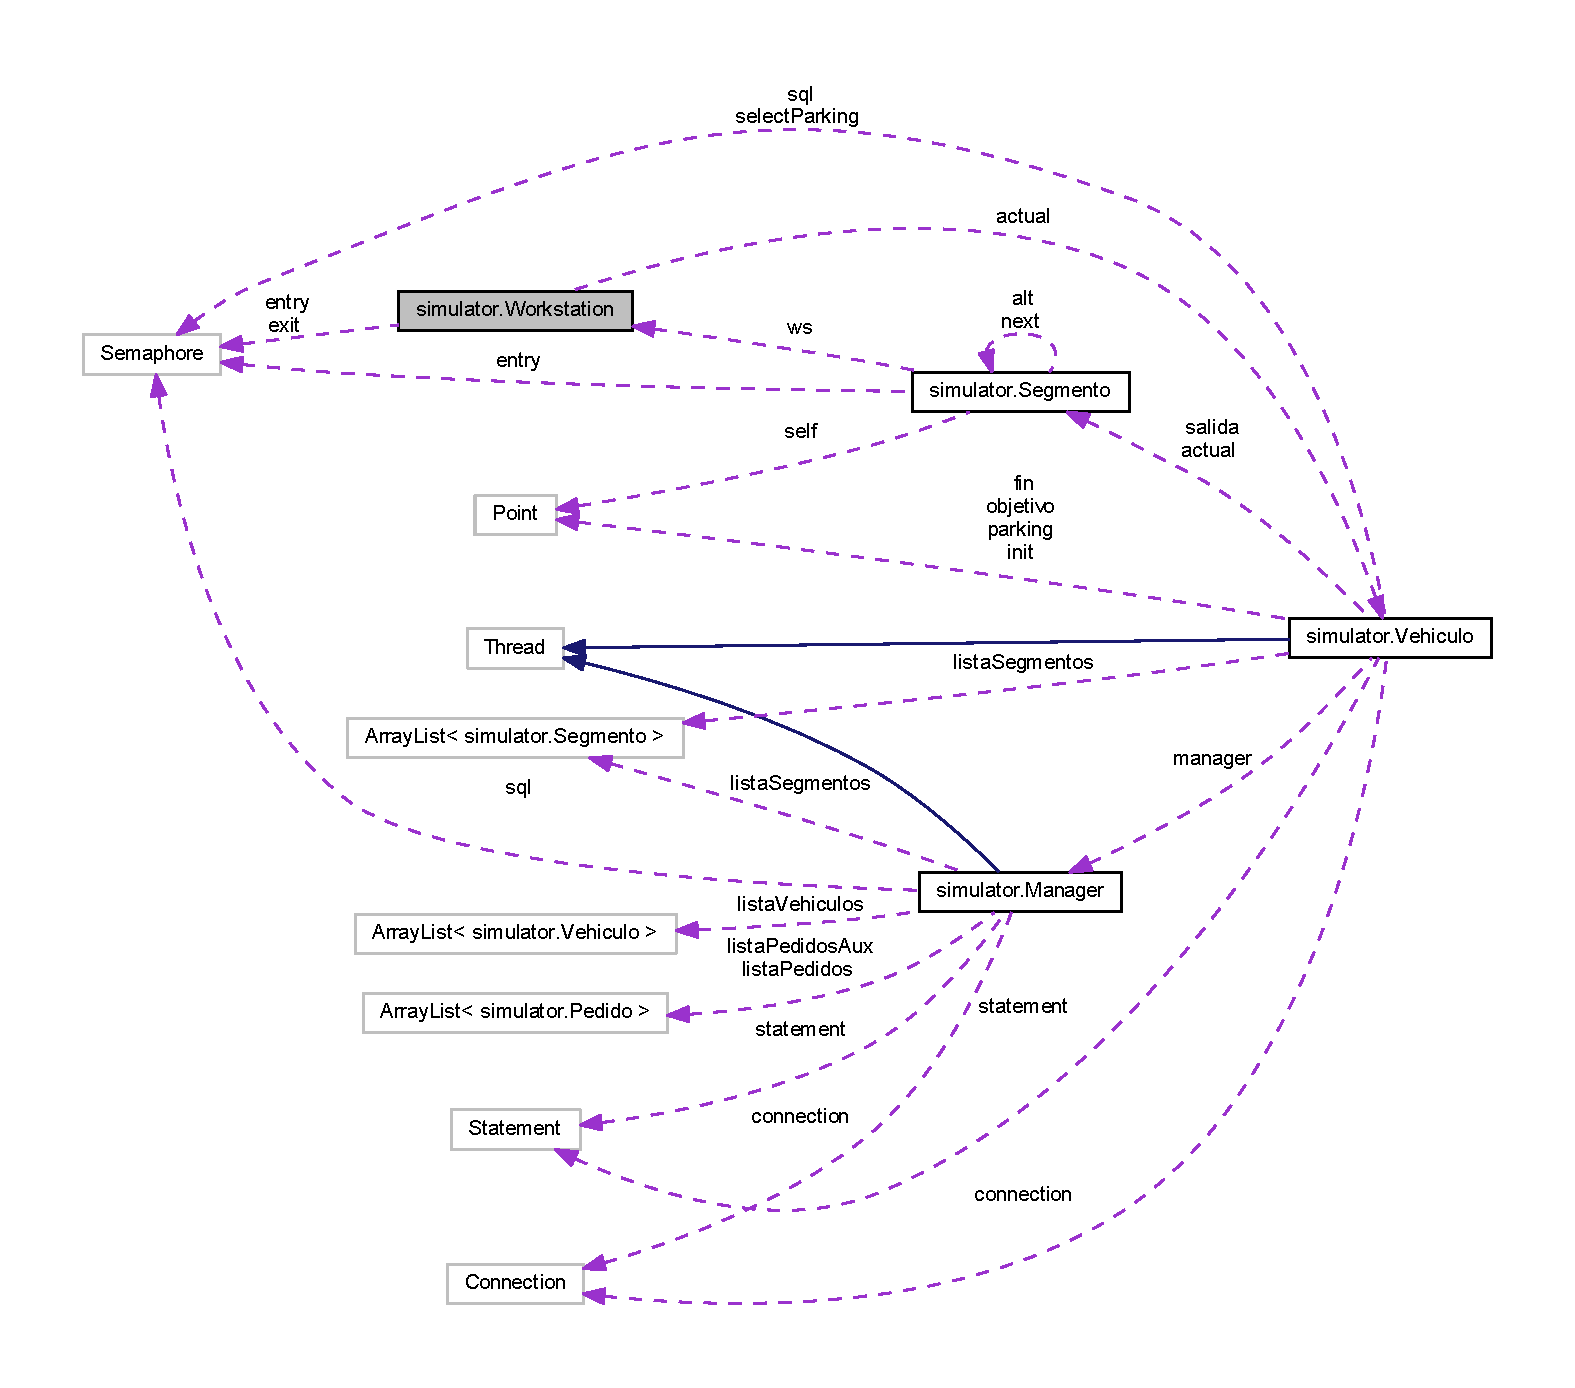
\includegraphics[width=350pt]{classsimulator_1_1_workstation__coll__graph}
\end{center}
\end{figure}
\subsection*{Public Member Functions}
\begin{DoxyCompactItemize}
\item 
\mbox{\hyperlink{classsimulator_1_1_workstation_a8b60b663f6370c910ec1ffaa84f464bb}{Workstation}} (String nombre)
\item 
Semaphore \mbox{\hyperlink{classsimulator_1_1_workstation_a0d389f9b0ca28ff6648467370afdb858}{get\+Exit}} ()
\item 
void \mbox{\hyperlink{classsimulator_1_1_workstation_a8807fa5c10a39810306359971abd58f0}{set\+Exit}} (Semaphore exit)
\item 
Semaphore \mbox{\hyperlink{classsimulator_1_1_workstation_af1001364022448a27a66b864376cdeff}{get\+Entry}} ()
\item 
void \mbox{\hyperlink{classsimulator_1_1_workstation_a1addeff99cf0ca9aaa020fe328a4f3fd}{set\+Entry}} (Semaphore entry)
\item 
boolean \mbox{\hyperlink{classsimulator_1_1_workstation_a9a306b4b5b6b740f9d284903c0f0eda4}{is\+Ocupado}} ()
\item 
void \mbox{\hyperlink{classsimulator_1_1_workstation_abc348d8ecea62cb7893d861ccc041c86}{set\+Ocupado}} (boolean ocupado)
\item 
\mbox{\hyperlink{classsimulator_1_1_vehiculo}{Vehiculo}} \mbox{\hyperlink{classsimulator_1_1_workstation_a017b4b43beb08ad12645ff2278543b49}{get\+Actual}} ()
\item 
void \mbox{\hyperlink{classsimulator_1_1_workstation_acf19a56acc88e29bdc0a394287eb6108}{set\+Actual}} (\mbox{\hyperlink{classsimulator_1_1_vehiculo}{Vehiculo}} actual)
\end{DoxyCompactItemize}


\subsection{Detailed Description}
This is the Worksation class The class contains the name, two Semaphores, a state of occupation and a vehicle

\begin{DoxyAuthor}{Author}
Joseba Carnicero, Aitor Eizmendi, Jon Mugica and Marcos Azkarate 
\end{DoxyAuthor}


Definition at line 11 of file Workstation.\+java.



\subsection{Constructor \& Destructor Documentation}
\mbox{\Hypertarget{classsimulator_1_1_workstation_a8b60b663f6370c910ec1ffaa84f464bb}\label{classsimulator_1_1_workstation_a8b60b663f6370c910ec1ffaa84f464bb}} 
\index{simulator\+::\+Workstation@{simulator\+::\+Workstation}!Workstation@{Workstation}}
\index{Workstation@{Workstation}!simulator\+::\+Workstation@{simulator\+::\+Workstation}}
\subsubsection{\texorpdfstring{Workstation()}{Workstation()}}
{\footnotesize\ttfamily simulator.\+Workstation.\+Workstation (\begin{DoxyParamCaption}\item[{String}]{nombre }\end{DoxyParamCaption})}



Definition at line 18 of file Workstation.\+java.



\subsection{Member Function Documentation}
\mbox{\Hypertarget{classsimulator_1_1_workstation_a017b4b43beb08ad12645ff2278543b49}\label{classsimulator_1_1_workstation_a017b4b43beb08ad12645ff2278543b49}} 
\index{simulator\+::\+Workstation@{simulator\+::\+Workstation}!get\+Actual@{get\+Actual}}
\index{get\+Actual@{get\+Actual}!simulator\+::\+Workstation@{simulator\+::\+Workstation}}
\subsubsection{\texorpdfstring{get\+Actual()}{getActual()}}
{\footnotesize\ttfamily \mbox{\hyperlink{classsimulator_1_1_vehiculo}{Vehiculo}} simulator.\+Workstation.\+get\+Actual (\begin{DoxyParamCaption}{ }\end{DoxyParamCaption})}



Definition at line 47 of file Workstation.\+java.

\mbox{\Hypertarget{classsimulator_1_1_workstation_af1001364022448a27a66b864376cdeff}\label{classsimulator_1_1_workstation_af1001364022448a27a66b864376cdeff}} 
\index{simulator\+::\+Workstation@{simulator\+::\+Workstation}!get\+Entry@{get\+Entry}}
\index{get\+Entry@{get\+Entry}!simulator\+::\+Workstation@{simulator\+::\+Workstation}}
\subsubsection{\texorpdfstring{get\+Entry()}{getEntry()}}
{\footnotesize\ttfamily Semaphore simulator.\+Workstation.\+get\+Entry (\begin{DoxyParamCaption}{ }\end{DoxyParamCaption})}



Definition at line 31 of file Workstation.\+java.

\mbox{\Hypertarget{classsimulator_1_1_workstation_a0d389f9b0ca28ff6648467370afdb858}\label{classsimulator_1_1_workstation_a0d389f9b0ca28ff6648467370afdb858}} 
\index{simulator\+::\+Workstation@{simulator\+::\+Workstation}!get\+Exit@{get\+Exit}}
\index{get\+Exit@{get\+Exit}!simulator\+::\+Workstation@{simulator\+::\+Workstation}}
\subsubsection{\texorpdfstring{get\+Exit()}{getExit()}}
{\footnotesize\ttfamily Semaphore simulator.\+Workstation.\+get\+Exit (\begin{DoxyParamCaption}{ }\end{DoxyParamCaption})}



Definition at line 23 of file Workstation.\+java.

\mbox{\Hypertarget{classsimulator_1_1_workstation_a9a306b4b5b6b740f9d284903c0f0eda4}\label{classsimulator_1_1_workstation_a9a306b4b5b6b740f9d284903c0f0eda4}} 
\index{simulator\+::\+Workstation@{simulator\+::\+Workstation}!is\+Ocupado@{is\+Ocupado}}
\index{is\+Ocupado@{is\+Ocupado}!simulator\+::\+Workstation@{simulator\+::\+Workstation}}
\subsubsection{\texorpdfstring{is\+Ocupado()}{isOcupado()}}
{\footnotesize\ttfamily boolean simulator.\+Workstation.\+is\+Ocupado (\begin{DoxyParamCaption}{ }\end{DoxyParamCaption})}



Definition at line 39 of file Workstation.\+java.

\mbox{\Hypertarget{classsimulator_1_1_workstation_acf19a56acc88e29bdc0a394287eb6108}\label{classsimulator_1_1_workstation_acf19a56acc88e29bdc0a394287eb6108}} 
\index{simulator\+::\+Workstation@{simulator\+::\+Workstation}!set\+Actual@{set\+Actual}}
\index{set\+Actual@{set\+Actual}!simulator\+::\+Workstation@{simulator\+::\+Workstation}}
\subsubsection{\texorpdfstring{set\+Actual()}{setActual()}}
{\footnotesize\ttfamily void simulator.\+Workstation.\+set\+Actual (\begin{DoxyParamCaption}\item[{\mbox{\hyperlink{classsimulator_1_1_vehiculo}{Vehiculo}}}]{actual }\end{DoxyParamCaption})}



Definition at line 51 of file Workstation.\+java.

\mbox{\Hypertarget{classsimulator_1_1_workstation_a1addeff99cf0ca9aaa020fe328a4f3fd}\label{classsimulator_1_1_workstation_a1addeff99cf0ca9aaa020fe328a4f3fd}} 
\index{simulator\+::\+Workstation@{simulator\+::\+Workstation}!set\+Entry@{set\+Entry}}
\index{set\+Entry@{set\+Entry}!simulator\+::\+Workstation@{simulator\+::\+Workstation}}
\subsubsection{\texorpdfstring{set\+Entry()}{setEntry()}}
{\footnotesize\ttfamily void simulator.\+Workstation.\+set\+Entry (\begin{DoxyParamCaption}\item[{Semaphore}]{entry }\end{DoxyParamCaption})}



Definition at line 35 of file Workstation.\+java.

\mbox{\Hypertarget{classsimulator_1_1_workstation_a8807fa5c10a39810306359971abd58f0}\label{classsimulator_1_1_workstation_a8807fa5c10a39810306359971abd58f0}} 
\index{simulator\+::\+Workstation@{simulator\+::\+Workstation}!set\+Exit@{set\+Exit}}
\index{set\+Exit@{set\+Exit}!simulator\+::\+Workstation@{simulator\+::\+Workstation}}
\subsubsection{\texorpdfstring{set\+Exit()}{setExit()}}
{\footnotesize\ttfamily void simulator.\+Workstation.\+set\+Exit (\begin{DoxyParamCaption}\item[{Semaphore}]{exit }\end{DoxyParamCaption})}



Definition at line 27 of file Workstation.\+java.

\mbox{\Hypertarget{classsimulator_1_1_workstation_abc348d8ecea62cb7893d861ccc041c86}\label{classsimulator_1_1_workstation_abc348d8ecea62cb7893d861ccc041c86}} 
\index{simulator\+::\+Workstation@{simulator\+::\+Workstation}!set\+Ocupado@{set\+Ocupado}}
\index{set\+Ocupado@{set\+Ocupado}!simulator\+::\+Workstation@{simulator\+::\+Workstation}}
\subsubsection{\texorpdfstring{set\+Ocupado()}{setOcupado()}}
{\footnotesize\ttfamily void simulator.\+Workstation.\+set\+Ocupado (\begin{DoxyParamCaption}\item[{boolean}]{ocupado }\end{DoxyParamCaption})}



Definition at line 43 of file Workstation.\+java.



The documentation for this class was generated from the following file\+:\begin{DoxyCompactItemize}
\item 
java/main/java/simulator/\mbox{\hyperlink{_workstation_8java}{Workstation.\+java}}\end{DoxyCompactItemize}

\chapter{File Documentation}
\hypertarget{_lista_segmento_8java}{}\section{java/main/java/simulator/\+Lista\+Segmento.java File Reference}
\label{_lista_segmento_8java}\index{java/main/java/simulator/\+Lista\+Segmento.\+java@{java/main/java/simulator/\+Lista\+Segmento.\+java}}
\subsection*{Classes}
\begin{DoxyCompactItemize}
\item 
class \mbox{\hyperlink{classsimulator_1_1_lista_segmento}{simulator.\+Lista\+Segmento}}
\end{DoxyCompactItemize}
\subsection*{Packages}
\begin{DoxyCompactItemize}
\item 
package \mbox{\hyperlink{namespacesimulator}{simulator}}
\end{DoxyCompactItemize}

\hypertarget{_manager_8java}{}\section{java/main/java/simulator/\+Manager.java File Reference}
\label{_manager_8java}\index{java/main/java/simulator/\+Manager.\+java@{java/main/java/simulator/\+Manager.\+java}}
\subsection*{Classes}
\begin{DoxyCompactItemize}
\item 
class \mbox{\hyperlink{classsimulator_1_1_manager}{simulator.\+Manager}}
\end{DoxyCompactItemize}
\subsection*{Packages}
\begin{DoxyCompactItemize}
\item 
package \mbox{\hyperlink{namespacesimulator}{simulator}}
\end{DoxyCompactItemize}

\hypertarget{_pedido_8java}{}\section{java/main/java/simulator/\+Pedido.java File Reference}
\label{_pedido_8java}\index{java/main/java/simulator/\+Pedido.\+java@{java/main/java/simulator/\+Pedido.\+java}}
\subsection*{Classes}
\begin{DoxyCompactItemize}
\item 
class \mbox{\hyperlink{classsimulator_1_1_pedido}{simulator.\+Pedido}}
\end{DoxyCompactItemize}
\subsection*{Packages}
\begin{DoxyCompactItemize}
\item 
package \mbox{\hyperlink{namespacesimulator}{simulator}}
\end{DoxyCompactItemize}

\hypertarget{_principal_8java}{}\section{java/main/java/simulator/\+Principal.java File Reference}
\label{_principal_8java}\index{java/main/java/simulator/\+Principal.\+java@{java/main/java/simulator/\+Principal.\+java}}
\subsection*{Classes}
\begin{DoxyCompactItemize}
\item 
class \mbox{\hyperlink{classsimulator_1_1_principal}{simulator.\+Principal}}
\end{DoxyCompactItemize}
\subsection*{Packages}
\begin{DoxyCompactItemize}
\item 
package \mbox{\hyperlink{namespacesimulator}{simulator}}
\end{DoxyCompactItemize}

\hypertarget{_producto_8java}{}\section{java/main/java/simulator/\+Producto.java File Reference}
\label{_producto_8java}\index{java/main/java/simulator/\+Producto.\+java@{java/main/java/simulator/\+Producto.\+java}}
\subsection*{Classes}
\begin{DoxyCompactItemize}
\item 
class \mbox{\hyperlink{classsimulator_1_1_producto}{simulator.\+Producto}}
\end{DoxyCompactItemize}
\subsection*{Packages}
\begin{DoxyCompactItemize}
\item 
package \mbox{\hyperlink{namespacesimulator}{simulator}}
\end{DoxyCompactItemize}

\hypertarget{_segmento_8java}{}\section{java/main/java/simulator/\+Segmento.java File Reference}
\label{_segmento_8java}\index{java/main/java/simulator/\+Segmento.\+java@{java/main/java/simulator/\+Segmento.\+java}}
\subsection*{Classes}
\begin{DoxyCompactItemize}
\item 
class \mbox{\hyperlink{classsimulator_1_1_segmento}{simulator.\+Segmento}}
\end{DoxyCompactItemize}
\subsection*{Packages}
\begin{DoxyCompactItemize}
\item 
package \mbox{\hyperlink{namespacesimulator}{simulator}}
\end{DoxyCompactItemize}

\hypertarget{_vehiculo_8java}{}\section{java/main/java/simulator/\+Vehiculo.java File Reference}
\label{_vehiculo_8java}\index{java/main/java/simulator/\+Vehiculo.\+java@{java/main/java/simulator/\+Vehiculo.\+java}}
\subsection*{Classes}
\begin{DoxyCompactItemize}
\item 
class \mbox{\hyperlink{classsimulator_1_1_vehiculo}{simulator.\+Vehiculo}}
\end{DoxyCompactItemize}
\subsection*{Packages}
\begin{DoxyCompactItemize}
\item 
package \mbox{\hyperlink{namespacesimulator}{simulator}}
\end{DoxyCompactItemize}

\hypertarget{_workstation_8java}{}\section{java/main/java/simulator/\+Workstation.java File Reference}
\label{_workstation_8java}\index{java/main/java/simulator/\+Workstation.\+java@{java/main/java/simulator/\+Workstation.\+java}}
\subsection*{Classes}
\begin{DoxyCompactItemize}
\item 
class \mbox{\hyperlink{classsimulator_1_1_workstation}{simulator.\+Workstation}}
\end{DoxyCompactItemize}
\subsection*{Packages}
\begin{DoxyCompactItemize}
\item 
package \mbox{\hyperlink{namespacesimulator}{simulator}}
\end{DoxyCompactItemize}

\hypertarget{_manager_test_8java}{}\section{java/test/java/test/\+Manager\+Test.java File Reference}
\label{_manager_test_8java}\index{java/test/java/test/\+Manager\+Test.\+java@{java/test/java/test/\+Manager\+Test.\+java}}
\subsection*{Classes}
\begin{DoxyCompactItemize}
\item 
class \mbox{\hyperlink{classtest_1_1_manager_test}{test.\+Manager\+Test}}
\end{DoxyCompactItemize}
\subsection*{Packages}
\begin{DoxyCompactItemize}
\item 
package \mbox{\hyperlink{namespacetest}{test}}
\end{DoxyCompactItemize}

\hypertarget{_pedido_test_8java}{}\section{java/test/java/test/\+Pedido\+Test.java File Reference}
\label{_pedido_test_8java}\index{java/test/java/test/\+Pedido\+Test.\+java@{java/test/java/test/\+Pedido\+Test.\+java}}
\subsection*{Classes}
\begin{DoxyCompactItemize}
\item 
class \mbox{\hyperlink{classtest_1_1_pedido_test}{test.\+Pedido\+Test}}
\end{DoxyCompactItemize}
\subsection*{Packages}
\begin{DoxyCompactItemize}
\item 
package \mbox{\hyperlink{namespacetest}{test}}
\end{DoxyCompactItemize}

\hypertarget{_producto_test_8java}{}\section{java/test/java/test/\+Producto\+Test.java File Reference}
\label{_producto_test_8java}\index{java/test/java/test/\+Producto\+Test.\+java@{java/test/java/test/\+Producto\+Test.\+java}}
\subsection*{Classes}
\begin{DoxyCompactItemize}
\item 
class \mbox{\hyperlink{classtest_1_1_producto_test}{test.\+Producto\+Test}}
\end{DoxyCompactItemize}
\subsection*{Packages}
\begin{DoxyCompactItemize}
\item 
package \mbox{\hyperlink{namespacetest}{test}}
\end{DoxyCompactItemize}

\hypertarget{_vehicles_test_8java}{}\section{java/test/java/test/\+Vehicles\+Test.java File Reference}
\label{_vehicles_test_8java}\index{java/test/java/test/\+Vehicles\+Test.\+java@{java/test/java/test/\+Vehicles\+Test.\+java}}
\subsection*{Classes}
\begin{DoxyCompactItemize}
\item 
class \mbox{\hyperlink{classtest_1_1_vehicles_test}{test.\+Vehicles\+Test}}
\end{DoxyCompactItemize}
\subsection*{Packages}
\begin{DoxyCompactItemize}
\item 
package \mbox{\hyperlink{namespacetest}{test}}
\end{DoxyCompactItemize}

%--- End generated contents ---

% Index
\backmatter
\newpage
\phantomsection
\clearemptydoublepage
\addcontentsline{toc}{chapter}{Index}
\printindex

\end{document}
